 %%% Laboratory	 Notes
%%% Template by Mikhail Klassen, April 2013
%%% Contributions from Sarah Mount, May 2014
%%% Contributions from Muhammad Davi, September 2022
\documentclass[a4paper]{tufte-handout}
\usepackage{lab_notes}

\title{Practice Big Data}
\date{2022}

\begin{document}
\maketitle

%%%%%%%%%%%%%%%%%%%%%%%%%%%%%%%%%%%%%%%%%%%%%%%%%%%%%%%%

\begin{projects}
\begin{description}
\item [Muhammad Davi, S.Kom., M.Cs.] adalah sebagai dosen pengampu matakuliah practice big data\footnote{Dosen Prodi Teknologi Rekayasa Komputer Jaringan, Jurusan Teknologi Informasi dan Komputer, Politeknik Negeri Lhokseumawe}.
\item [Peserta dan Kelompok] matakuliah practice big data adalah sebegai berikut:

\begin{table}[!ht]
\caption{Peserta dan Kelompok Matakuliah Practice Big Bata}
\label{tab:peserta}
\centering
\begin{tabular}{ll} 
\toprule
Nama &	Akun Github\\
\midrule
Kelompok 1\\
\midrule
Adinda Awaliah			& \url{https://github.com/AdindaAwaliah} \\
Adjie Yusmunandar		& \url{https://github.com/AdjieYusmunandar} \\
Arya Saputra			& \url{https://github.com/AryaSpt} \\
Jihan Dwi Sarah			& \url{https://github.com/jhndsrh} \\
\midrule
Kelompok 2\\
\midrule
Muhammad Munawir		& \url{https://github.com/Munawir027} \\
Muhammad Ikrammullah	& \url{https://github.com/Ikram160302} \\
M. Ikhsan				& \url{https://github.com/Muhammadikhsandev} \\
Zulfahmi				& \url{https://github.com/zulfahmidev} \\
\midrule
Kelompok 3\\
\midrule
Nadzura Kumaira			& \url{https://github.com/NadzuraKumaira} \\
Nurani Harum Fardaniah	& \url{https://github.com/fardaniahnh} \\
Nuraula Tafiza			& \url{https://github.com/olala17} \\
Nurul Aflah				& \url{https://github.com/Nurulaflahhh} \\
Faiza Yuwafiqi			& \url{https://github.com/faizayuwafiqi} \\
\midrule
Kelompok 4\\
\midrule
Rauzatinur Syah			& \url{https://github.com/rauzatinursyah} \\
Resha Russita			& \url{https://github.com/resharussita} \\
Rizki Ilhami			& \url{https://github.com/RIZKIINC} \\
Taravia Fauzah			& \url{https://github.com/traviafzah} \\
\midrule
Kelompok 5\\
\midrule
Salsabila Irmanda		& \url{https://github.com/salsabilairmanda17} \\
Siti Hajar Al Zahra		& \url{https://github.com/sitihjralzahara} \\
Syarfani Akbar			& \url{https://github.com/SyarfaniAkbar} \\
Cut Opy Mandalisa		& \url{https://github.com/cutopymdl} \\
\midrule
\end{tabular}
\end{table}
\end{description}
\end{projects}

%%%%%%%%%%%%%%%%%%%%%%%%%%%%%%%%%%%%%%%%%%%%%%%%%%%%%%%%

\begin{maybe}
\begin{itemize}
\item Waktu, Tempat dan Penilaian

\begin{itemize}
\item Waktu: 13.30 - 16.00, 16.20 - 18.00\footnote{Istirahat dan Sholat Ashar 20 Menit}
\item Tempat: Ruang Lab 3\footnote{Lab Jaringan dan Multimedia di Lantai Dasar Gedung Utama}
\item Penilaian\footnote{Sesuai ketentuan dari Kepala Lab}

\begin{multicols}{2}
\begin{itemize}
\item Responsi Kompetensi
\item Sikap
\item Laporan
\item Seminar
\item UAS
\item Hasil/Benda kerja
\end{itemize}
\end{multicols}
\end{itemize}

\item Sebelum masuk lab wajib berbaris dan berdo'a terlebih dahulu di depan lab.
\item Sebelum perkuliahan dimulai, mahasiswa atau yang mewakili memberi laporan.
\item Setiap keluar lab meminta izin kepada dosen pengampu.
\item Mengikuti Tata Tertib yang berlaku.
\item Referensi

\begin{itemize}
\item Buku Ajar Big Data \citep{Mursyidah2020}.
\end{itemize}

\item Tata Cara Presensi selama Perkuliahan Online

\begin{itemize}
\item Buka repository laporan-practice-big-data melalui akun GitHub masing-masing
\item Lakukan sinkro fork (Sync fork)
\item Buka file {\tt lab\_notes.tex} menggunakan texmaker dan buka file laporan masing-masing
\item Tambahkan kode berikut dan sesuaikan tanggalnya. \\
\textbf{\textcolor{red}{Pastikan kode sudah benar!}}
\begin{lstlisting}
\newday{\textbf{1 Desember 2022}}
\begin{enumerate}
	\item Kendala dan Solusi
	\item Kesimpulan
\end{enumerate}
\end{lstlisting}
\item Lakukan {\tt git add, git commit dan git push}. \\ 
Format \textit{message} saat {\tt git commit} \textit{"Presensi dd-mm-yyyy a.n. Nama"}. Contoh: "Presensi 01-12-2022 a.n. Davi"
\item Buat {\tt pull requests} melalui menu \textbf{Contribute}.
\end{itemize}
\end{itemize}
\end{maybe}

%%%%%%%%%%%%%%%%%%%%%%%%%%%%%%%%%%%%%%%%%%%%%%%%%%%%%%%%
\clearpage
\newday{\#1 - 8 September 2022}

\newthought{Introduction \& Preparation}

Pada pertemuan pertama, kegiatan lab adalah perkenalan dan persiapan kebutuhan untuk praktik big data. Setelah dosen pengampu memperkenalkan diri dan matakuliah yang diajarkan, dilanjutkan perkenalan dari setiap mahasiswa dah hasilnya dapat dilihat pada Tabel \ref{tab:perkenalan}.

\begin{table}[!ht]
\vspace*{.5cm}
\caption{Data Mahasiswa}
\label{tab:perkenalan}
\centering
\begin{tabular}{cllr} 
\toprule
No & Nama 				& Asal Sekolah 				& Alamat\\
\midrule
1 	& Adinda Awaliah	& SMA N 1 Lhokseumawe 		& Cunda \\
2 	& Adjie Yusmunandar	& SMK N 1 Lhokseumawe 		& Paloh Lada \\
3 	& Arya Saputra 		& SMK N 2 Lhokseumawe 		& Blang Pulo \\
4 	& Cut Opy Mandalisa	& SMA N 1 Syamtalira Bayu	& Bayu \\
5 	& Faiza Yuwafiqi	& SMK N 3 Lhokseumawe 		& Panggoi \\
6 	& Jihan Dwi Sarah	& SMA N 1 Lhokseumawe 		& Panggoi \\
7 	& M. Ikhsan			& SMK N 1 Simpang Kiri 		& Subulussalam \\
\midrule
8 	& Muhammad Ikrammullah		& SMK N 1 Lhokseumawe 	& Banda Sakti \\
9 	& Muhammad Munawir			& SMK N 1 Lhoksukon		& Karing Meurah Mulia \\
10 	& Nadzura Kumaira			& SMK N 2 Lhokseumawe 	& Keude Aceh \\
11 	& Nurani Harum Fardaniah	& SMK N 1 Lhoksukon 	& Buket Hagu \\
12 	& Nuraula Tafiza			& SMK N 1 Lhoksukon 	& Alue Buket \\
13 	& Nurul Aflah				& MAS Syamsuddhuha		& Glp. Sulu Barat \\
14 	& Rauzatinur Syah			& MAS Misbahul Ulum 	& Geudong \\
\midrule
15 	& Resha Russita			& SMA N 1 Lhokseumawe 	& Alue Awe \\
16 	& Rizki Ilhami			& SMK N 1 Lhoksukon 	& Lapang \\
17 	& Salsabila Irmanda		& MAS Misbahul Ulum 	& Alue Awe \\
18 	& Siti Hajar Al Zahra	& MAN 4 Aceh Utara 		& Blang Jruen \\
19 	& Syarfani Akbar		& SMK N 1 Lhokseumawe 	& Uten Bayi \\
20 	& Taravia Fauzah		& SMA N 1 Dewantara 	& Blang Naleung Mameh \\
21 	& Zulfahmi				& SMK N 1 Lhokseumawe	& Kuta Makmur \\
\bottomrule
\end{tabular}
\end{table}

\vspace*{.5cm}
Setelah perkenalan, setiap mahasiswa membuat akun github dan akun discord sebagai media komunikasi dan tempat bekerja secara berkelompok. Hasil dari kegiatan tersebut dapat dilihat pada Tabel \ref{tab:peserta} dan Link Server Discord, yaitu \url{https://discord.gg/bJCNpaxv62}.

Tugas di pertemuan pertama adalah menyiapkan \textit{environment} untuk tempat kerja minimal sebagai berikut:
\begin{multicols}{2}
\begin{itemize}
\setlength\itemsep{0em}
\item Processor 2 GHz dual-core
\item RAM sebesar 4 GB
\item Harddisk kosong 25 GB
\item Resolusi layar 1024 x 768
\item \textit{Operating System}: Ubuntu 22.04 LTS
\end{itemize}
\end{multicols}
\hrulefill

%%%%%%%%%%%%%%%%%%%%%%%%%%%%%%%%%%%%%%%%%%%%%%%%%%%%%%%%
\clearpage
\newday{\#2 - 15 September 2022}

\newthought{Instalasi dan Konfigurasi GIT dengan GitHub}

Pada pertemuan kali ini kita belajar install GIT dan konfigurasi GIT dengan GitHub agar dapat menjalankan perintah-perintah GIT melalui lokal dan menyimpan hasil kerjaan kita ke GitHub. Karena pada pertemuan pertama telah membuat akun GitHub, maka pada pertemuan kali ini asumsinya semua sudah memiliki akun GitHub. Setelah itu ikuti beberapa langkah berikut untuk praktikum kali ini.

\begin{enumerate}
\item Install Git \\
Pertema download program Git melalui link ini (\url{https://git-scm.com/download}) sesuai dengan sistem operasi yang digunakan. Bagi pengguna Windows jika proses download sudah selesai, lanjut proses instalasi seperti program windows pada umumnya (Next, Next, Next, sampai selesai).

\item \textit{Generate} SSH-Key \\
Jika instalasi sudah selesai, coba buka Git Bash, maka akan muncul program baru yang mirip dengan Terminal atau Command Prompt (CMD) kita sebut Git Bash. Kemudian jalankan perintah berikut untuk \textit{generate ssh-key}.

{\tt ssh-keygen -t ed25519 -C "email@akun.github"} \\

Ganti {\tt email@akun.github} dengan email yang terdaftar pada akun GitHub. Selanjutnya jika muncul beberapa pertanyaan seperti berikut ini tekan [enter].

{\tt > Enter a file in which to save the key (/Users/YOU/.ssh/id\_ed25519:} \\
{\tt > Enter passphrase (empty for no passphrase):} \\
{\tt > Enter same passphrase again:}

Jika proses diatas berhasil maka terbentuk folder baru dengan nama {\tt .ssh}. Didalam folder tersebut terdapat \textit{private key} dan \textit{public key}. Bukan file \textit{public key} (id\_ed25519.pub) dan \textit{copy} isi dari file tersebut.

\item Menambahkan SSH-Key ke Akun GitHub \\
Untuk menambahkan SSH-Key ke akun GitHub pertama login terlebih dahulu. Setelah berhasil login klik pada gambar profil sehingga tampil menu dropdown seperti pada Gambar \ref{gam:langkah-ssh} nomor 1. Selanjutnya pilih menu \textbf{Setting} sepertin yang ditunukan pada nomor 2. Setelah memilih menu \textbf{Setting} maka muncul halaman setting dengan menu di sidebar sebelah kiri. Pada menu sebelah kiri pilih menu \textbf{SSH and GPG keys} seperti pada nomor 3. Kemudian klik tombol \textbf{New SSH key} maka akan muncul form menambahkan SSH seperti yang diperlihatkan pada Gambar \ref{gam:form-ssh}.

\begin{figure}[!ht]
\includegraphics[width=\textwidth]{gtihub-1}
\caption{Lankah-langkah Menambah SSH-Key di GitHub}
\label{gam:langkah-ssh}
\end{figure}

Kode SSH-Key yang telah di-\textit{copy} pada langkah sebelumnya \textit{paste}-kan kode tersebut pada isian \textbf{Key} dan beri judul SSH-Key pada isian \textbf{Title}. Setelah semua diisi klik tombol \textbf{Add SSH key} untuk menyimpan SSH-Key baru tersebut.

\begin{figure}[!ht]
\includegraphics[width=\textwidth]{github-2}
\caption{Form Penambahan SSH-Key di GitHub}
\label{gam:tambah-ssh}
\end{figure}

Untuk menguji bahwa penambahan SSH-Key telah berhasil coba lakukan {\tt git push} untuk repositori laporan practice big data dari akun masing-masing. Untuk lebih jelasnya tentang GIT dapat membaca catatan pada link berikut \url{https://muhdavi.github.io/learn-git/}.
\end{enumerate}

\begin{figure}[!ht]
\includegraphics[width=.95\textwidth]{24-11-2022}
\caption{Perkuliahan Daring via Google Meet}
\label{gam:perkuliahan-24-11}
\end{figure}

\vspace*{-.5cm}
\hrulefill

%%%%%%%%%%%%%%%%%%%%%%%%%%%%%%%%%%%%%%%%%%%%%%%%%%%%%%%%
\clearpage
\newday{\#3 - 22 September 2022}
\newday{\#4 - 24 November 2022 menggantikan 29 September 2022}
\newday{\#5 - 25 November 2022 menggantikan 6 Oktober 2022}

\newthought{Instalasi dan Konfigurasi GIT dengan GitHub - Lanjutan}

Mahasiswa yang sudah berhasil konfigurasi Git dengan GitHub dan melakukan {\tt Pull Request}:
\begin{multicols}{2}
\begin{enumerate}
\item Rizki Ilhami
\item Rauzatinur Syah $\star$
\item Taravia Fauzah
\item Resha Russita $\star$
\item Nurani Harum Fardaniah $\star$
\item Adinda Awaliah $\star$
\item Salsabila Irmanda $\star$
\item M. Ikhsan
\item Jihan Dwi Sarah $\star$
\item Cut Opy Mandalisa $\star$
\item Zulfahmi
\item Muhammad Munawir
\item Nuraula Tafiza
\item Muhammad Ikrammullah
\item Nadzura Kumaira
\item Adjie Yusmunandar
\item Nurul Aflah
\item Arya Saputra
\item Faiza Yuwafiqi
\item Siti Hajar Al Zahra
\item Syarfani Akbar
\end{enumerate}
\end{multicols}

\begin{figure}[!ht]
\includegraphics[width=\textwidth]{25-11-2022}
\caption{Perkuliahan Daring via Google Meet}
\label{gam:perkuliahan-25-11}
\end{figure}

\vspace*{-.5cm}
\hrulefill

%%%%%%%%%%%%%%%%%%%%%%%%%%%%%%%%%%%%%%%%%%%%%%%%%%%%%%%%
\clearpage
\newday{\#6 - 1 Desember 2022 menggantikan 13 Oktober 2022
\footnote{Mahasiswa yang hadir:
\begin{enumerate}
\item Adinda Awaliah
\item Arya Saputra $\oplus$
\item Cut Opy Mandalisa
\item Jihan Dwi Sarah
\item M. Ikhsan
\item Muhammad Ikrammullah
\item Muhammad Munawir
\item Nadzura Kumaira
\item Nurani Harum Fardaniah
\item Rauzatinur Syah
\item Resha Russita
\item Rizki Ilhami
\item Salsabila Irmanda
\item Syarfani Akbar
\item Taravia Fauzah
\item Zulfahmi
\end{enumerate}}}

\newthought{Instalasi Apache Hadoop}

Pada pertemuan kedua ini kegiatan yang dilakukan adalah menginstall Apache Hadoop pada \textit{environment} yang telah dibuat pada pertemuan sebelumnya. Untuk menginstall Apache Hadoop dapat mengikut langkah-langkah berikut ini:

\begin{enumerate}
\item Membuat Group dan User Baru
\begin{itemize}
\item Membuat group \\
{\tt sudo addgroup hadoop}
\item Membuat User Baru dan Menambahkan ke Group \\
{\tt sudo adduser -ingroup hadoop hdfs}
\item Ubah Hak Akses \\
{\tt sudo visudo}
\item Tambahkan Kode \\
{\tt hdfs	ALL=(ALL:ALL) ALL}
\item Ganti ke User Baru \\
{\tt su - hdfs}
\end{itemize}

\item Install Java \\
{\tt sudo apt update} \\
{\tt sudo apt install openjdk-8-jdk -y} \\

\item Verifikasi Hasil Instalasi Java \\
{\tt java -version} \\
Jika instalasi java berhasil tanpa ada bug atau error maka akan menampilkan hasil seperti pada Gambar \ref{gam:java-version}.

\begin{figure}
\setlength{\belowcaptionskip}{-10pt}
\includegraphics[width=\textwidth]{java-version}
\caption{Versi Java yang Terinstall}
\label{gam:java-version}
\end{figure}

\item Setting SSH \\
\begin{itemize}
\item Uninstall OpenSSH \\
{\tt sudo apt remove openssh-server openssh-client}
\item Install OpenSSH Baru \\
{\tt sudo apt update} \\
{\tt sudo apt install openssh-server openssh-client} \\
{\tt sudo ufw allow 22} \\
{\tt sudo systemctl restart ssh} \\
{\tt sudo apt install ssh} \\
{\tt sudo apt install rsync}
\item Generate Key \\
{\tt ssh-keygen -t dsa -P '' -f $\sim$/.ssh/id\_dsa} \\
{\tt cat $\sim$/.ssh/id\_dsa.pub >> $\sim$/.ssh/authorized\_keys} \\
{\tt ssh-keygen -t rsa}
\item Coba Masuk via SSH \\
{\tt ssh localhost}
\item Jika masih harus memasukkan password, lanjutkan langakh berikut. \\
{\tt ssh-keygen -t rsa} \\
{\tt cat $\sim$/.ssh/id\_rsa.pub >> $\sim$/.ssh/authorized\_keys} \\
{\tt chmod og-wx $\sim$/.ssh/authorized\_keys} \\
{\tt sudo apt update}
\item Coba Masuk via SSH Lagi \\
{\tt ssh localhost}
\item Jika sudah berhasil, keluar dengan perintah {\tt exit} \\
{\tt exit}
\end{itemize}

\item Download Apache Hadoop \\
{\tt wget https://dlcdn.apache.org/hadoop/common/hadoop-3.3.4/hadoop-3.3.4.tar.gz}

\item Ekstrak Apache Hadoop \\
{\tt tar -xzvf hadoop-3.3.4.tar.gz }
\begin{itemize}
\item x $\Rightarrow$ ekstrak file arsip.
\item z $\Rightarrow$ filter file arsip melalui gzip.
\item v $\Rightarrow$ menampilkan proses.
\item f $\Rightarrow$ nama file arsip.
\end{itemize}

\item Pindahkan hasil ekstraksi ke {\tt /usr/local/} \\
{\tt sudo mv hadoop-3.3.4 /usr/local/hadoop}

\item Ubah Hak Akses {\tt /usr/local/hadoop} \\
{\tt sudo chown -R hdfs:hadoop /usr/local/hadoop} \\
{\tt sudo chmod -R 777 /usr/local/hadoop}

\item Edit file {\tt sysctl.conf} untuk Disable IPV6
\begin{itemize}
\item Buka file {\tt sysctl.conf} \\
{\tt sudo nano /etc/sysctl.conf}
\item Tambahkan Kode
\begin{lstlisting}
net.ipv6.conf.all.disable_ipv6=1
net.ipv6.conf.lo.disable_ipv6=1
net.ipv6.conf.default_ipv6=1
\end{lstlisting}
\end{itemize}

\item Edit file {\tt hadoop-env.sh} \\
{\tt cd /usr/local/hadoop/etc/hadoop} \\
{\tt sudo nano hadoop-env.sh} \\

\begin{lstlisting}
export JAVA_HOME=/usr/lib/jvm/java-8-openjdk-amd64
export HADOOP_OPTS=-Djava.net.preferIPv4Stack=true
export HADOOP_HOME_WARN_SUPPRESS="TRUE"
export HADOOP_ROOT_LOGGER="WARN"
\end{lstlisting}

\item Menambahkan Hadoop ke {\tt .bashrc} \\
{\tt sudo nano $\sim$/.bashrc} \\
\begin{lstlisting}
#Hadoop Location
export HADOOP_HOME=/usr/local/hadoop
export HADOOP_CONF_DIR=/usr/local/hadoop/etc/hadoop
export HADOOP_MAPRED_HOME=/usr/local/hadoop
export HADOOP_COMMON_HOME=/usr/local/hadoop
export HADOOP_HDFS_HOME=/usr/local/hadoop
export YARN_HOME=/usr/local/hadoop
export PATH=$PATH:/usr/local/hadoop/bin
export PATH=$PATH:/usr/local/hadoop/sbin

#Hadoop Native Location
export HADOOP_COMMON_LIB_NATIVE_DIR=$HADOOP_HOME/lib/native
export HADOOP_OPTS="$HADOOP_OPTS -Djava.library.path=$HADOOP_HOME/lib/native"
export LD_LIBRARY_PATH=$HADOOP_HOME/lib/native
\end{lstlisting}

{\tt source .bashrc}

\item Verifikasi Hasil Instalasi Hadoop \\
{\tt hadoop version} \\
Jika instalasi hadoop berhasil, maka ketika mengecek versi hadoop akan muncul seperti yang diperlihatkan pada Gambar \ref{gam:hadoop-version}.
\begin{figure}[!ht]
\includegraphics[width=\textwidth]{hadoop-version}
\caption{Versi Hadoop Terinstall 3.3.4}
\label{gam:hadoop-version}
\end{figure}
\end{enumerate}
 
\hrulefill

%%%%%%%%%%%%%%%%%%%%%%%%%%%%%%%%%%%%%%%%%%%%%%%%%%%%%%%%
\clearpage
\newday{\#7 - 2 Desember 2022 menggantikan 20 Oktober 2022
\footnote{Mahasiswa yang hadir:
\begin{enumerate}
\item Muhammad Munawir
\item Rizki Ilhami
\item Rauzatinur Syah
\item Salsabila Irmanda
\item Adjie Yusmunandar
\item Nurani Harum Fardaniah
\item Cut Opy Mandalisa
\item Resha Russita
\item Taravia Fauzah
\item Adinda Awaliah
\item Jihan Dwi Sarah
\item M. Ikhsan
\item Zulfahmi
\end{enumerate}}}

\newthought{Konfigurasi Apache Hadoop}

Setelah selesai meng-install Hadoop, kita perlu konfigurasi beberapa file Hadoop agar memudahkan kita dalam memonitoring ekosistem Hadoop yang telah diinstall.

\begin{enumerate}
\item Konfigurasi File Hadoop \\
Beberapa file Hadoop yang perlu dikonfigurasi berada pada folder {\tt hadoop/etc/hadoop} seperti yang diperlihatkan pada Gambar \ref{gam:file-hadoop}. Konfigurasi file-file tersebut dapat menggunakan {\tt nano} diikuti nama file. Sisipkan kode konfigurasi diantara tag {\tt <configuration> $\cdots$ </configuration>}.

\begin{figure}[!ht]
\includegraphics[width=\textwidth]{file-hadoop}
\caption{File Konfigurasi Hadoop}
\label{gam:file-hadoop}
\end{figure}

Berikut bebrapa file yang perlu dikonfigurasi dan lakukan dengan hati-hati serta teliti malalui perintah berikut:

{\tt cd /usr/local/hadoop/etc/hadoop} \\
{\tt sudo nano nama-file}

\begin{itemize}

\item {\tt sudo nano core-site.xml}
\begin{lstlisting}
<property>
	<name>hadoop.tmp.dir</name>
	<value>/app/hadoop/tmp</value>
</property>
<property>
	<name>fs.default.name</name>
	<value>hdfs://localhost:9000</value>
</property>
\end{lstlisting}

\item {\tt sudo nano hdfs-site.xml}
\begin{lstlisting}
<property>
	<name>dfs.replication</name>
	<value>1</value>
</property>
<property>
	<name>dfs.namenode.name.dir</name>
	<value>file:/usr/local/hadoop/yarn_data/hdfs/namenode</value>
</property>
<property>
	<name>dfs.datanode.data.dir</name>
	<value>file:/usr/local/hadoop/yarn_data/hdfs/datanode</value>
</property>
\end{lstlisting}

\item {\tt sudo nano mapred-site.xml}
\begin{lstlisting}
<property>
	<name>mapred.framework.name</name>
	<value>yarn</value>
</property>
<property>
	<name>mapreduce.jobhistory.address</name>
	<value>localhost:10020</value>
</property>
\end{lstlisting}

\item {\tt sudo nano yarn-site.xml}
\begin{lstlisting}
<property>
	<name>yarn.nodemanager.aux-services</name>
	<value>mapreduce_shuffle</value>
</property>
<property>
	<name>yarn.nodemanager.aux-services.mapreduce.shuffle.class</name>
	<value>org.apache.hadoop.mapred.ShuffleHandler</value>
</property>
\end{lstlisting}
\end{itemize}

\item Membuat Folder Sementara (\textit{Temporary}) untuk HDFS \\
{\tt sudo mkdir -p /app/hadoop/tmp} \\
{\tt sudo chmod -R 777 /app/hadoop/tmp} \\
{\tt sudo chown -R hdfs:hadoop /app/hadoop/tmp}

\item Membuat Folder {\tt namenode} dan {\tt datanode} \\
{\tt sudo mkdir -p /usr/local/hadoop/yarn\_data/hdfs/namenode} \\
{\tt sudo mkdir -p /usr/local/hadoop/yarn\_data/hdfs/datanode} \\
{\tt sudo chown -R hdfs:hadoop /usr/local/hadoop/yarn\_data/hdfs/namenode} \\
{\tt sudo chown -R hdfs:hadoop /usr/local/hadoop/yarn\_data/hdfs/datanode} \\
{\tt sudo chmod -R 777 /usr/local/hadoop/yarn\_data/hdfs/namenode} \\
{\tt sudo chmod -R 777 /usr/local/hadoop/yarn\_data/hdfs/datanode}

\item Jalankan Perintah Format HDFS \\
{\tt hdfs namenode -format}

\item Jalankan Hadoop Service \\
{\tt start-dfs.sh} \\
{\tt start-yarn.sh} \\

\item Cek Hadoop Service
\begin{itemize}
\item Jalankan perintah {\tt jps}
\item Akses melalui web browser dengan alamat \url{http://localhost:9870}\footnote{Seperti yang diperlihatkan pada Gambar \ref{gam:namenode}} atau \url{http://localhost:8088}\footnote{Seperti yang diperlihatkan pada Gambar \ref{gam:resourcemanager}}.
\end{itemize}

\begin{figure}[!ht]
\includegraphics[width=\textwidth]{namenode}
\label{gam:namenode}
\end{figure}
\vspace*{-.7cm}
\begin{figure}[!ht]
\includegraphics[width=\textwidth]{resourcemanager}
\caption{Resource Manager Hadoop}
\label{gam:resourcemanager}
\end{figure}

\vspace*{-.7cm}
\item Hentikan Hadoop Service
\begin{itemize}
\item Hentikan Service Tertentu \\
{\tt stop-dfs.sh} atau {\tt stop-yarn.sh}
\item Hentikan Semua Service \\
{\tt stop-all.sh}
\end{itemize}
\end{enumerate}
% mounting data shared folder
% sudo mount -t vboxsf share /mnt/share

\vspace*{.1cm}
\hrulefill

%%%%%%%%%%%%%%%%%%%%%%%%%%%%%%%%%%%%%%%%%%%%%%%%%%%%%%%%
\clearpage
\newday{\#8 - 8 Desember 2022 menggantikan 3 November 2022
\footnote{Mahasiswa yang hadir:
\begin{enumerate}
\item Adinda Awaliah
\item Adjie Yusmunandar
%\item Arya Saputra
\item Cut Opy Mandalisa
%\item Faiza Yuwafiqi
\item Jihan Dwi Sarah
\item M. Ikhsan
\item Muhammad Ikrammullah
\item Muhammad Munawir
%\item Nadzura Kumaira
\item Nurani Harum Fardaniah
%\item Nuraula Tafiza
%\item Nurul Aflah
\item Rauzatinur Syah
\item Resha Russita
\item Rizki Ilhami
\item Salsabila Irmanda
%\item Siti Hajar Al Zahra
%\item Syarfani Akbar
\item Taravia Fauzah
\item Zulfahmi
\end{enumerate}}}

\newday{\#9 - 9 Desember 2022 menggantikan 10 November 2022
\footnote{Mahasiswa yang hadir:
\begin{enumerate}
\item Adinda Awaliah
\item Adjie Yusmunandar
%\item Arya Saputra
\item Cut Opy Mandalisa
%\item Faiza Yuwafiqi
\item Jihan Dwi Sarah
\item M. Ikhsan
%\item Muhammad Ikrammullah
\item Muhammad Munawir
%\item Nadzura Kumaira
\item Nurani Harum Fardaniah
%\item Nuraula Tafiza
%\item Nurul Aflah
\item Rauzatinur Syah
\item Resha Russita
\item Rizki Ilhami
\item Salsabila Irmanda
%\item Siti Hajar Al Zahra
%\item Syarfani Akbar
\item Taravia Fauzah
\item Zulfahmi
\end{enumerate}}}

\newthought{Instalasi Apache Hadoop - Lanjutan}

\noindent
Mahasiswa yang sudah berhasil install Apache Hadoop:
\begin{multicols}{2}
\begin{enumerate}
\item Taravia Fauzah
\item Jihan Dwi Sarah
\item Salsabila Irmanda
\item Rauzatinur Syah
\item Resha Russita
\item Nurani Harum Fardaniah
\item Rizki Ilhami
\item Cut Opy Mandalisa
\end{enumerate}
\end{multicols}

\noindent
Mahasiswa yang sedang progress install Apache Hadoop :
\begin{multicols}{2}
\begin{enumerate}
\item Muhammad Ikrammullah
\item Zulfahmi
\item M. Ikhsan
\item Adjie Yusmunandar
\item Muhammad Munawir
\item Adinda Awaliah
\end{enumerate}
\end{multicols}

\noindent
Berikut mahasiswa yang belum terlihat progress::
\begin{multicols}{2}
\begin{enumerate}
\item Arya Saputra
\item Faiza Yuwafiqi
\item Nadzura Kumaira
\item Nuraula Tafiza
\item Nurul Aflah
\item Siti Hajar Al Zahra
\item Syarfani Akbar
\end{enumerate}
\end{multicols}

\hrulefill

%%%%%%%%%%%%%%%%%%%%%%%%%%%%%%%%%%%%%%%%%%%%%%%%%%%%%%%%
\clearpage
\newday{\#10 - 15 Desember 2022 menggantikan 10 November 2022
\footnote{Mahasiswa yang hadir:
\begin{enumerate}
\item Adinda Awaliah
\item Adjie Yusmunandar
\item Arya Saputra
\item Cut Opy Mandalisa
\item Faiza Yuwafiqi
\item Jihan Dwi Sarah
\item M. Ikhsan
\item Muhammad Ikrammullah
\item Muhammad Munawir
\item Nadzura Kumaira
\item Nurani Harum Fardaniah
%\item Nuraula Tafiza
\item Nurul Aflah
\item Rauzatinur Syah
\item Resha Russita
\item Rizki Ilhami
\item Salsabila Irmanda
%\item Siti Hajar Al Zahra
%\item Syarfani Akbar
\item Taravia Fauzah
%\item Zulfahmi
\end{enumerate}}}

\newthought{Program WordCount bawaan Hadoop}

Jika sudah selesai malakukan instalasi Hadoop, maka dapat mencoba program bawaan Hadoop untuk memahami bagaimana proses dan cara kerja Hadoop dalam memproses data input hingga menghasilkan sebuah output. Salah satu program yang sudah disediakan oleh Hadoop adalah WordCount, yaitu program menghitung jumlah kata dalam data input yang dibarikan. Silahkan ikuti langkah-langkah berikut ini untuk mengetahui cara penggunaan program WordCount.

\begin{enumerate}
\item Jalankan Hadoop Service \\
{\tt start-dfs.sh} \\
{\tt yarn-dfs.sh}

\item Buat folder input di HDFS\\
{\tt hadoop fs -mkdir /input}

\item Buat file baru dengan nama dan data berikut \\
{\tt nano dataWordCount.txt}
\begin{lstlisting}
AdindaAwaliah, SMA_N_1_Lhokseumawe, Cunda
AdjieYusmunandar, SMK_N_1_Lhokseumawe, Paloh_Lada
AryaSaputra, SMK_N_2_Lhokseumawe, Blang_Pulo
CutOpyMandalisa, SMA_N_1_Syamtalira_Bayu, Bayu
FaizaYuwafiqi, SMK_N_3_Lhokseumawe, Panggoi
JihanDwiSarah, SMA_N_1_Lhokseumawe, Panggoi
M.Ikhsan, SMK_N_1_Simpang_Kiri, Subulussalam
MuhammadIkrammullah, SMK_N_1_Lhokseumawe, Banda_Sakti
MuhammadMunawir, SMK_N_1_Lhoksukon, Karing_Meurah_Mulia
NadzuraKumaira, SMK_N_2_Lhokseumawe, Keude_Aceh
NuraniHarumFardaniah, SMK_N_1_Lhoksukon, Buket_Hagu
NuraulaTafiza, SMK_N_1_Lhoksukon, Alue_Buket
NurulAflah, MAS_Syamsuddhuha, Glp._Sulu_Barat
RauzatinurSyah, MAS_Misbahul_Ulum, Geudong
ReshaRussita, SMA_N_1_Lhokseumawe, Alue_Awe
RizkiIlhami, SMK_N_1_Lhoksukon, Lapang
SalsabilaIrmanda, MAS_Misbahul_Ulum, Alue_Awe
SitiHajarAlZahra, MAN_4_Aceh_Utara, Blang_Jruen
SyarfaniAkbar, SMK_N_1_Lhokseumawe, Uten_Bayi
TaraviaFauzah, SMA_N_1_Dewantara, Blang_Naleung_Mameh
Zulfahmi, SMK_N_1_Lhokseumawe, Kuta_Makmur
\end{lstlisting}

\item Pindahkan file {\tt dataWordCount.txt} ke folder input di HDFS \\
{\tt hadoop fs -put dataWordCount.txt /input}

\item Jalankan program WordCount \\
{\tt hadoop jar /usr/local/hadoop/share/hadoop/mapreduce/hadoop-mapreduce-examples-3.3.4.jar wordcount /input/dataWordCount.txt /output}
%hadoop jar /usr/local/hadoop/share/hadoop/mapreduce/hadoop-mapreduce-examples-3.2.0.jar wordcount /input/ /output2 -> untuk semua file dari folder input

\item Cek Hasil \\
{\tt hadoop fs -ls /output}

\item Lihat Hasil \\
{\tt hadoop fs -cat /output/part-r-00000}
\end{enumerate}

\newthought{Tugas Praktikum} \\
Screenshot hasil dari langkah 6 dan 7 dan masukkan ke dalam laporan. Kumpulkan melalui {\tt pull requests} dengan format pesan "\textit{Laporan dd-mm-yyyy an. Nama}".

\hrulefill

%%%%%%%%%%%%%%%%%%%%%%%%%%%%%%%%%%%%%%%%%%%%%%%%%%%%%%%%
\clearpage
\newday{\#11 - 16 Desember 2022 menggantikan 17 November 2022
\footnote{Mahasiswa yang hadir:
\begin{enumerate}
\item Adinda Awaliah
\item Adjie Yusmunandar
%\item Arya Saputra
%\item Cut Opy Mandalisa
\item Faiza Yuwafiqi
\item Jihan Dwi Sarah
\item M. Ikhsan
%\item Muhammad Ikrammullah
%\item Muhammad Munawir
%\item Nadzura Kumaira
\item Nurani Harum Fardaniah
\item Nuraula Tafiza
\item Nurul Aflah
\item Rauzatinur Syah
\item Resha Russita
\item Rizki Ilhami
\item Salsabila Irmanda
%\item Siti Hajar Al Zahra
%\item Syarfani Akbar
\item Taravia Fauzah
\item Zulfahmi
\end{enumerate}}}

\newthought{Program WordCount dengan Java}

Pada pertemuan sebelumnya telah mencoba program WordCount bawaan Hadoop. Jika dengan program bawaan Hadoop sudah dapat mendapatkan hasil, artinya Hadoop kita sudah bisa digunakan untuk menjalankan program. Ikuti beberapa langkah berikut untuk memberikan pemahaman bagaimana proses membuat program, menyiapkan data, meng-compile program hingga menjalankan program dan memperoleh hasilnya.

\begin{enumerate}
\item Pastikan Hadoop Service sudah berjalan
\item Pastikan data input pada pertemuan sebelumnya masih tersedia di HDFS

{\tt hadoop fs -ls /input}

\item Buat file baru dengan nama dan kode berikut \\

{\tt sudo nano WordCount.java}
\begin{lstlisting}
import java.io.IOException;
import java.util.StringTokenizer;
import org.apache.hadoop.conf.Configuration;
import org.apache.hadoop.fs.Path;
import org.apache.hadoop.io.IntWritable;
import org.apache.hadoop.io.Text;
import org.apache.hadoop.mapreduce.Job;
import org.apache.hadoop.mapreduce.Mapper;
import org.apache.hadoop.mapreduce.Reducer;
import org.apache.hadoop.mapreduce.lib.input.FileInputFormat;
import org.apache.hadoop.mapreduce.lib.output.FileOutputFormat;

public class WordCount {
	public static class TokenizerMapper extends Mapper<Object, Text, Text, IntWritable> {
    	private final static IntWritable one = new IntWritable(1);
        private Text word = new Text();
        public void map(Object key, Text value, Context context) throws IOException, InterruptedException {
            StringTokenizer itr = new StringTokenizer(value.toString());
            while (itr.hasMoreTokens()) {
                word.set(itr.nextToken());
                context.write(word, one);
            }
        }
    }

    public static class IntSumReducer extends Reducer<Text, IntWritable, Text, IntWritable> {
        private IntWritable result = new IntWritable();
        public void reduce(Text key, Iterable<IntWritable> values, Context context) throws IOException, InterruptedException {
            int sum = 0;
            for (IntWritable val : values) {
                sum += val.get();
            }
            result.set(sum);
            context.write(key, result);
        }
    }

    public static void main(String[] args) throws Exception {
        Configuration conf = new Configuration();
        Job job = Job.getInstance(conf, "word count");
        job.setJarByClass(WordCount.class);
        job.setMapperClass(TokenizerMapper.class);
        job.setCombinerClass(IntSumReducer.class);
        job.setReducerClass(IntSumReducer.class);
        job.setOutputKeyClass(Text.class);
        job.setOutputValueClass(IntWritable.class);
        FileInputFormat.addInputPath(job, new Path(args[0]));
        FileOutputFormat.setOutputPath(job, new Path(args[1]));
        System.exit(job.waitForCompletion(true) ? 0 : 1);
    }
}
\end{lstlisting}
% https://github.com/muhdavi/kode-practice-big-data/blob/main/WordCountJava/src/main/java/WordCount.java

\item Buat classpath \\
{\tt export HADOOP\_CLASSPATH=\$(\$HADOOP\_HOME/bin/hadoop classpath)}

\item Buat folder baru untuk menampung hasil \textit{compile} program java dan ubah hak aksesnya \\
{\tt sudo mkdir JavaCompiled} \\
{\tt sudo chmod -R 777 JavaCompiled}

\item Compile file WordCount.java \\
{\tt \small{javac -classpath \$HADOOP\_CLASSPATH -d JavaCompiled/WordCount.java}}

\item Mengubah file menjadi executable .jar \\
{\tt jar -cvf WordCount.jar -C JavaCompiled/ .}

\item Jalankan program WordCount \\
{\tt \footnotesize{hadoop jar WordCount.jar WordCount /input/dataWordCount.txt /ResultWordCountJava}}

\item Cek Hasil \\
{\tt hadoop fs -ls /ResultWordCountJava}

\item Lihat Hasil \\
{\tt hadoop fs -cat /ResultWordCountJava/part-r-00000}
\end{enumerate}

\newthought{Tugas Praktikum} \\
Screenshot hasil dari langkah 9 dan 10 serta masukkan ke dalam laporan. Kumpulkan melalui {\tt pull requests} dengan format pesan "\textit{Laporan dd-mm-yyyy an. Nama}".

\hrulefill

%%%%%%%%%%%%%%%%%%%%%%%%%%%%%%%%%%%%%%%%%%%%%%%%%%%%%%%%
\clearpage
\newday{\#12 - 22 Desember 2022 menggantikan 24 November 2022
\footnote{Mahasiswa yang hadir:
\begin{enumerate}
\item Adinda Awaliah
\item Adjie Yusmunandar
\item Arya Saputra
\item Cut Opy Mandalisa
%\item Faiza Yuwafiqi
\item Jihan Dwi Sarah
\item M. Ikhsan
%\item Muhammad Ikrammullah
\item Muhammad Munawir
\item Nadzura Kumaira
\item Nurani Harum Fardaniah
\item Nuraula Tafiza
\item Nurul Aflah
\item Rauzatinur Syah
\item Resha Russita
\item Rizki Ilhami
\item Salsabila Irmanda
\item Siti Hajar Al Zahra
\item Syarfani Akbar
\item Taravia Fauzah
\item Zulfahmi
\end{enumerate}}}

\newthought{Instalasi Apache Spark (PySpark)}

\begin{enumerate}
\item Download Apache Spark \\
{\tt \footnotesize{wget https://dlcdn.apache.org/spark/spark-3.3.1/spark-3.3.1-bin-hadoop3.tgz}}

\item Ekstrak Apache Spark \\
{\tt tar -xzvf spark-3.3.1-bin-hadoop3.tgz}

\item Pindahkan hasil ekstraksi ke {\tt /usr/local/} \\
{\tt sudo mv spark-3.3.1-bin-hadoop3 /usr/local/spark}

\item Menambahkan Spark ke {\tt .bashrc} \\
{\tt sudo nano $\sim$/.bashrc}
\begin{lstlisting}
#Spark Location
export SPARK_HOME=/usr/local/spark
export PATH=$PATH:$SPARK_HOME/bin:$SPARK_HOME/sbin
\end{lstlisting}
{\tt source $\sim$/.bashrc}

\item Verifikasi Hasil Instalasi Spark

{\tt pyspark ---version}

\begin{figure}[!ht]
\includegraphics[width=\textwidth]{spark-version}
\caption{Versi Spark Terinstall 3.3.1 }
\label{gam:form-ssh}
\end{figure}

\item Jalankan Spark Service \\
{\tt start-master.sh}

\item Hentikan Spark Service \\
{\tt stop-master.sh}
\end{enumerate}

\newthought{Tugas Praktikum} \\
Screenshot hasil dari langkah 5 dan masukkan ke dalam laporan. Kumpulkan melalui {\tt pull requests} dengan format pesan "\textit{Laporan dd-mm-yyyy an. Nama}".

\hrulefill

%%%%%%%%%%%%%%%%%%%%%%%%%%%%%%%%%%%%%%%%%%%%%%%%%%%%%%%%
\clearpage
\newday{\#13 - 23 Desember 2022 menggantikan 1 Desember 2022
\footnote{Mahasiswa yang hadir:
\begin{enumerate}
\item Adinda Awaliah
%\item Adjie Yusmunandar
%\item Arya Saputra
\item Cut Opy Mandalisa
\item Faiza Yuwafiqi
\item Jihan Dwi Sarah
\item M. Ikhsan
%\item Muhammad Ikrammullah
%\item Muhammad Munawir
%\item Nadzura Kumaira
\item Nurani Harum Fardaniah
%\item Nuraula Tafiza
%\item Nurul Aflah
\item Rauzatinur Syah
\item Resha Russita
\item Rizki Ilhami
\item Salsabila Irmanda
%\item Siti Hajar Al Zahra
%\item Syarfani Akbar
\item Taravia Fauzah
\item Zulfahmi
\end{enumerate}}}

\newthought{Program WordCount dengan Python}

\begin{enumerate}
\item Pastikan Hadoop Service dan Spark Service berjalan
\item Pastikan data input pada pertemuan sebelumnya masih tersedia di HDFS
\item Buat folder baru untuk menyimpan file Python \\
{\tt sudo mkdir WordCountPython} 

\item Buat file baru dengan nama dan kode berikut
\begin{itemize}
\item {\tt map.py} \\
{\tt sudo nano WordCountPython/map.py}
\begin{lstlisting}
#!/usr/bin/python

import sys

for line in sys.stdin:
    line = line.strip()
    words = line.split()
    for word in words:
        print('{}\t{}'.format(word, 1))
\end{lstlisting}
%{\tt wget https://raw.githubusercontent.com/muhdavi/kode-practice- big-data/main/WordCountPython/map.py}

\item {\tt reduce.py} \\
{\tt sudo nano WordCountPython/reduce.py}
\begin{lstlisting}
#!/usr/bin/python

import sys

current_count = 0
current_word = None
word = None

for line in sys.stdin:
    line = line.strip()
    word, count = line.split('\t', 1)

    try:
        count = int(count)
    except ValueError:
        continue

    if current_word == word:
        current_count += count
    else:
        if current_word:
            print('{}\t{}'.format(current_word, current_count))
        current_count = count
        current_word = word        

if current_word == word:
    print('{}\t{}'.format(current_word, current_count))
\end{lstlisting}
%{\tt wget https://raw.githubusercontent.com/muhdavi/kode-practice- big-data/main/WordCountPython/reduce.py}
\end{itemize}

\item Ubah Hak Akses \\
{\tt sudo chmod +x -R WordCountPython/} 

\item Mencoba Program di Local \\
{\tt echo jangan heran jika orang cantik merasa jelek sementara orang yang jelek merasa cantik | WordCountPython/map.py | sort | WordCountPython/reduce.py}


\item Jalankan Program menggunakan Hadoop \\
{\tt hadoop jar /usr/local/hadoop/share/hadoop/tools/lib/hadoop-streaming-3.3.4.jar -mapper $\sim$/WordCountPython/map.py -reducer $\sim$/WordCountPython/reduce.py -input /input/dataWordCount.txt -output /ResultWordCountPython}

\item Cek Hasil \\
{\tt hadoop fs -ls /ResultWordCountPython}

\item Lihat Hasil \\
{\tt hadoop fs -cat /ResultWordCountPython/part-00000}
\end{enumerate}

\vspace*{-.5cm}
\newthought{Tugas Praktikum} \\
Screenshot hasil dari langkah 8 dan 9 serta masukkan ke dalam laporan. Kumpulkan melalui {\tt pull requests} dengan format pesan "\textit{Laporan dd-mm-yyyy an. Nama}".

\hrulefill

%%%%%%%%%%%%%%%%%%%%%%%%%%%%%%%%%%%%%%%%%%%%%%%%%%%%%%%%
\clearpage
\newday{\#14 - 23 Desember 2022 menggantikan 8 Desember 2022}

\newthought{Program WordCount dengan PySpark}

\begin{enumerate}
\item Pastikan Hadoop Service dan Spark Service berjalan
\item Pastikan data input pada pertemuan sebelumnya masih tersedia di HDFS
\item Buat folder baru untuk menyimpan file Python \\
{\tt sudo mkdir WordCountPySpark} \\
{\tt cd WordCountPySpark}

\item Buat file baru dengan nama dan kode berikut \\
{\tt sudo nano WordCount.py}
\begin{lstlisting}
from pyspark.sql import SparkSession
spark = SparkSession.builder.master("local").appName('WordCount').getOrCreate()
sc = spark.sparkContext
sc.setLogLevel("ERROR")
# input data
data = sc.textFile("/input/dataWordCount.txt")
# process
counts = data.flatMap(lambda line: line.split(" ")).map(lambda word: (word, 1)).reduceByKey(lambda a, b: a + b)
# output
counts.saveAsTextFile("/ResultWordCountPySpark")
output = counts.collect()
for (word, count) in output:
    print("%s: %i" % (word, count))
\end{lstlisting}

\item Jalankan Program menggunakan PySpark \\
{\tt spark-submit WordCount.py}

\item Cek Hasil \\
{\tt hadoop fs -ls /ResultWordCountPyspark}

\item Lihat Hasil \\
{\tt hadoop fs -cat /ResultWordCountPyspark/part-00000}
\end{enumerate}

\vspace*{-.5cm}
\newthought{Tugas Praktikum} \\
Screenshot hasil dari langkah 6 dan 7 serta masukkan ke dalam laporan. Kumpulkan melalui {\tt pull requests} dengan format pesan "\textit{Laporan dd-mm-yyyy an. Nama}".

\hrulefill

%%%%%%%%%%%%%%%%%%%%%%%%%%%%%%%%%%%%%%%%%%%%%%%%%%%%%%%%
\clearpage
\newday{\#15 - Tugas Individu menggantikan 15 Desember 2022}

\newthought{Program Machine Learning dengan PySpark}

Berbeda dengan program sebelumnyan, program ini dijalankan satu-per-satu perintahnya di terminal PySpark. Ikutilah langkah-langkah berikut ini secara cermat dan teliti. Setiap perintah yang Anda kerjakan buat dokumentasi-nya dan Anda masukkan ke dalam Laporan dengan mengumpulkannya melalui GitHub dengan \textit{message "Laporan Tugas Mandiri a.n. Nama"}.

\begin{enumerate}
\item Pastikan Hadoop dan Spark berjalan
\item Pastikan package sudah tersedia \\
{\tt pip list}
\begin{multicols}{3}
\begin{itemize}
\item pandas
\item matplotlib
\item numpy
\item seaborn
\item scikit-learn
\end{itemize}
\end{multicols}

Jika package tersebut belum tersedia, install terlebih dahulu menggunakan {\tt pip}, misalnya {\tt pip install scikit-learn}.

\item Load Package \\
{\tt 
import numpy as np \\
import pandas as pd \\
import seaborn as sns \\
import matplotlib.pyplot as plt \\
from sklearn.datasets import load\_iris \\
from pyspark.sql import SparkSession \\
}

\item Load Data \\
{\tt
data\_iris = load\_iris(as\_frame=True) \\
df = pd.DataFrame(data\_iris.data, columns = data\_iris.feature\_names) \\
spark\_df = spark.createDataFrame(df) \\
spark\_df.show(5)
}

\item Menentukan nilai K dengan metode \textit{silhouette} \\
{\tt
from pyspark.ml.feature import VectorAssembler \\

assemble=VectorAssembler(inputCols=[\\
'sepal length (cm)',\\
'sepal width (cm)',\\
'petal length (cm)',\\
'petal width (cm)'],\\
outputCol = 'iris\_features')
}

{\tt
assembled\_data=assemble.transform(spark\_df) \\
assembled\_data.show(5) \\
from pyspark.ml.clustering import KMeans \\
from pyspark.ml.evaluation import ClusteringEvaluator \\

silhouette\_scores=[]
}

{\tt
evaluator = ClusteringEvaluator(featuresCol='iris\_features', metricName='silhouette', distanceMeasure='squaredEuclidean') \\
}

{\tt
for K in range(2,11): \\
\hspace*{7mm}KMeans\_=KMeans(featuresCol='iris\_features', k=K) \\
\hspace*{7mm}KMeans\_fit=KMeans\_.fit(assembled\_data) \\
\hspace*{7mm}KMeans\_transform=KMeans\_fit.transform(assembled\_data) \\
\hspace*{7mm}evaluation\_score=evaluator.evaluate(KMeans\_transform) \\
\hspace*{7mm}silhouette\_scores.append(evaluation\_score) \\

fig, ax = plt.subplots(1,1, figsize=(10,8)) \\
ax.plot(range(2,11), silhouette\_scores) \\
ax.set\_xlabel('Jumlah Cluster') \\
ax.set\_ylabel('Hasil Silhouette') \\
plt.show()
}

\item Membangun Model \textit{K-Means Clustering} \\
{\tt
KMeans\_=KMeans(featuresCol='iris\_features', k=3) \\
KMeans\_Model=KMeans\_.fit(assembled\_data) \\
KMeans\_Assignments=KMeans\_Model.transform(assembled\_data)
}

\item Menampilkan Hasil \textit{Clustering} dengan PCA \\
{\tt
from pyspark.ml.feature import PCA as PCAml \\
pca = PCAml(k=2, inputCol="iris\_features", outputCol="pca") \\
pca\_model = pca.fit(assembled\_data) \\
pca\_transform = pca\_model.transform(assembled\_data)
} 

{\tt
x\_pca = np.array(pca\_transform.rdd.map(lambda row: row.pca).collect())
}

{\tt
cluster\_assignment = np.array(KMeans\_Assignments.rdd.map(lambda row: row.prediction).collect()).reshape(-1,1)
}

{\tt
pca\_data = np.hstack((x\_pca,cluster\_assignment))
}

{\tt
pca\_df = pd.DataFrame(data=pca\_data, columns=("1st\_principal", "2nd\_principal","cluster\_assignment")) 
}

{\tt
sns.FacetGrid(pca\_df,hue="cluster\_assignment", height=6).map(plt.scatter, '1st\_principal', '2nd\_principal').add\_legend() \\
}

{\tt plt.show()}
\end{enumerate}

\hrulefill

%%%%%%%%%%%%%%%%%%%%%%%%%%%%%%%%%%%%%%%%%%%%%%%%%%%%%%%%
\clearpage
\newday{\#16 - Tugas Kelompok menggantikan 22 Desember 2022}

\newthought{Program Machine Learning dengan PySpark}

Berdasarakn program sebelumnya yang telah Anda coba malalui Terminal PySpark, kerjakan tugas berikut secara berkelompok:

\begin{enumerate}
\item Buatlah program tersebut dalam bentuk file Python sehingga dapat dijalankan menggunakan {\tt spark-submit}.
\item Dokumentasikan hasil dan perubahan yang Anda lakukan untuk dimasukkan ke dalam laporan.
\item Kumpulkan laporan beserta file Python melalui GitHub dengan format \textit{message "Laporan Kelompok Nomor-Kelompok}".
\item Kumpulkan file Python didalam folder yang telah disediakan \textit{TugasKelompok}. Yang mengumpulkan cukup salah satu sebagai perwakilan/ketua kelompok.
\end{enumerate}

\hrulefill

\begin{center}
\noindent
\textbf{\textcolor{red}{Ingat!\\ Semua Tugas dan Laporan panling lambat dikumpulkan tanggal 5 Januari 2023.}}
\end{center}

\hrulefill

%%%%%%%%%%%%%%%%%%%%%%%%%%%%%%%%%%%%%%%%%%%%%%%%%%%%%%%%
\clearpage
\newthought{Rekap Progres Praktikum}

\begin{table}[!ht]
\vspace*{.5cm}
\centering
\begin{tabular}{cl|c|c|c|c|c|c|c|c} 
	& & 
	\multirow{9}{*}{\rotatebox{90}{\parbox[l]{3.3cm}{Install Hadoop}}} &
	\multirow{9}{*}{\rotatebox{90}{\parbox[l]{3.3cm}{WordCount Hadoop}}} &
	\multirow{9}{*}{\rotatebox{90}{\parbox[l]{3.3cm}{WordCount Java}}} & 
	\multirow{9}{*}{\rotatebox{90}{\parbox[l]{3.3cm}{Install Apache Spark}}} &
	\multirow{9}{*}{\rotatebox{90}{\parbox[l]{3.3cm}{WordCount Python}}} &
	\multirow{9}{*}{\rotatebox{90}{\parbox[l]{3.3cm}{WordCount PySpark}}} &
	\multirow{9}{*}{\rotatebox{90}{\parbox[l]{3.3cm}{Tugas Individu}}} &
	\multirow{9}{*}{\rotatebox{90}{\parbox[l]{3.3cm}{Tugas Kelompok}}} \\
	& & & & & & & & & \\
	& & & & & & & & & \\
	& & & & & & & & & \\
	& & & & & & & & & \\
	& & & & & & & & & \\
	& & & & & & & & & \\
No 	& Nama 						& $\star$ & & & & & & & \\ \hline
1 	& Adinda Awaliah			& & & & & & & & \\ \hline
2 	& Adjie Yusmunandar			& & & & & & & & \\ \hline
3 	& Arya Saputra 				& & & & & & & & \\ \hline
4 	& Cut Opy Mandalisa			& $\star$ & $\star$ & $\star$ & & & & & \\ \hline
5 	& Faiza Yuwafiqi			& $\star$ & $\star$ & $\star$ & & & & & \\ \hline
6 	& Jihan Dwi Sarah			& $\star$ & $\star$ & $\star$ & $\star$ & $\star$ & $\star$ & & \\ \hline
7 	& M. Ikhsan					& & & & & & & & \\ \hline
8 	& Muhammad Ikrammullah		& & & & & & & & \\ \hline
9 	& Muhammad Munawir			& & & & & & & & \\ \hline
10 	& Nadzura Kumaira			& & & & & & & & \\ \hline
11 	& Nurani Harum Fardaniah	& $\star$ & $\star$ & $\star$ & $\star$ & & & & \\ \hline
12 	& Nuraula Tafiza			& & & & & & & & \\ \hline
13 	& Nurul Aflah				& & & & & & & & \\ \hline
14 	& Rauzatinur Syah			& $\star$ & $\star$ & $\star$ & $\star$ & $\star$ & $\star$ & $\star$ & \\ \hline
15 	& Resha Russita				& $\star$ & $\star$ & $\star$ & $\star$ & $\star$ & $\star$ & $\star$ & \\ \hline
16 	& Rizki Ilhami				& $\star$ & $\star$ & $\star$ & $\star$ & & & & \\ \hline
17 	& Salsabila Irmanda			& $\star$ & $\star$ & $\star$ & $\star$ & & & & \\ \hline
18 	& Siti Hajar Al Zahra		& & & & & & & & \\ \hline
19 	& Syarfani Akbar			& & & & & & & & \\ \hline
20 	& Taravia Fauzah			& $\star$ & $\star$ & $\star$ & $\star$ & $\star$ & $\star$ & & \\ \hline
21 	& Zulfahmi					& & & & & & & & \\ \hline
\multicolumn{2}{c|}{Perbandingan}		& 
$\frac{9}{12}$ &
$\frac{9}{12}$ &
$\frac{9}{12}$ &
$\frac{7}{14}$ &
$\frac{4}{17}$ &
$\frac{4}{17}$ &
$\frac{2}{19}$ &
$\frac{0}{21}$ \\
\end{tabular}
\end{table}

%\hrulefill

%%%%%%%%%%%%%%%%%%%%%%%%%%%%%%%%%%%%%%%%%%%%%%%%%%%%%%%%
\begin{comment}
\footnote{Mahasiswa yang hadir:
\begin{enumerate}
\item Adinda Awaliah
\item Adjie Yusmunandar
\item Arya Saputra
\item Cut Opy Mandalisa
\item Faiza Yuwafiqi
\item Jihan Dwi Sarah
\item M. Ikhsan
\item Muhammad Ikrammullah
\item Muhammad Munawir
\item Nadzura Kumaira
\item Nurani Harum Fardaniah
\item Nuraula Tafiza
\item Nurul Aflah
\item Rauzatinur Syah
\item Resha Russita
\item Rizki Ilhami
\item Salsabila Irmanda
\item Siti Hajar Al Zahra
\item Syarfani Akbar
\item Taravia Fauzah
\item Zulfahmi
\end{enumerate}}}
\end{comment}

%%%%%%%%%%%%%%%%%%%%%%%%%%%%%%%%%%%%%%%%%%%%%%%%%%%%%%%%

\newthought{\textbf{Adinda Awaliah - 2020903430004 - TRKJ 3B}}

\newday{\textbf{1-2 desember 2022} - Instalasi dan Konfigurasi Apache Hadoop}
\begin{enumerate}
\item Kendala dan Solusi
\newline praktikum instalasi apache hadoop tidak ada kendala. konfigurasi apache hadoop terkendala pada saat perintah jps, hasil yang muncul hanya 2jps, solusinya kembali ke langkah ssh, dan untuk menampilkan jps harus berada pada /usr/local/hadoop/etc/hadoop

\item Kesimpulan
\newline berhasil melakukan instalasi. berhasil melakukan konfigurasi.

\begin{figure}[!ht]
\includegraphics[width=\textwidth]{AdindaAwaliah/jps}
\caption{hasil dari jps}
\label{gam:jps}
\end{figure}

\begin{figure}
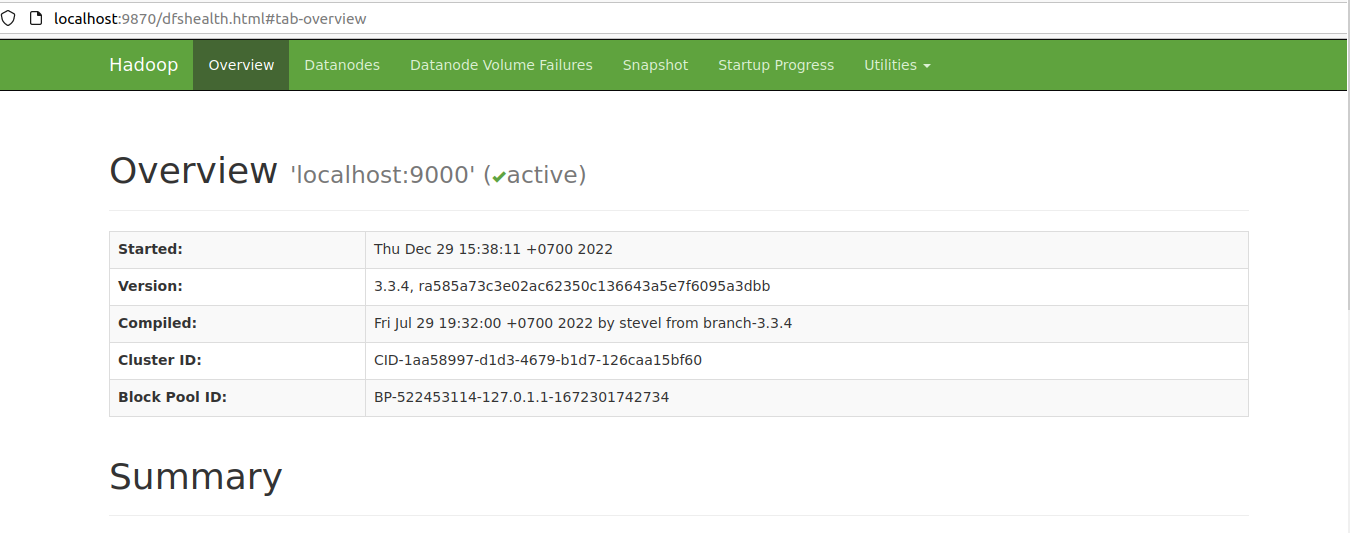
\includegraphics[width=\textwidth]{AdindaAwaliah/konfigurasi apache hadoop web 9870}
\caption{apache hadoop web 9870}
\label{gam:konfigurasi apache hadoop web 9870}
\end{figure}

\begin{figure}
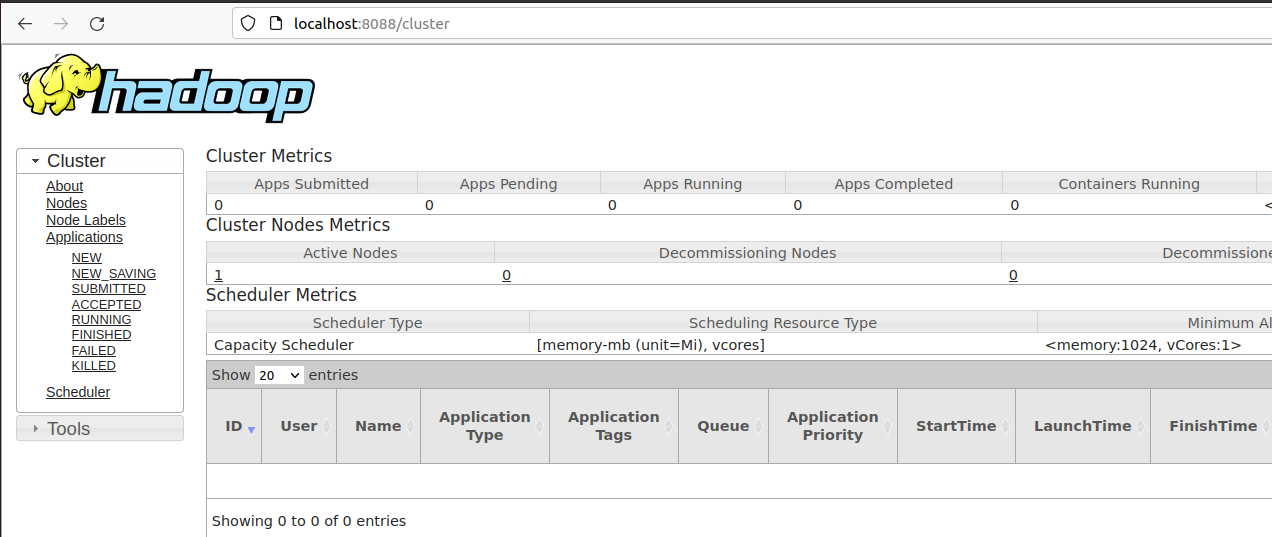
\includegraphics[width=\textwidth]{AdindaAwaliah/konfigurasi apache hadoop web 8088}
\caption{apache hadoop web 8088}
\label{gam:konfigurasi apache hadoop web 8088}
\end{figure}

\end{enumerate}

\newday{\textbf{ 8-9 desember 2022}}
\begin{enumerate}
\item Kendala dan Solusi
% jelaskan kendala dan penyebab yang dialami saat mengikuti praktikum serta solusi atau langkah-langkah yang telah dilakukan

\item Kesimpulan
% berikan kesimpulan dari praktikum yang telah dikerjkan
\newline lanjutan instalasi apache hadoop

\end{enumerate}


\newday{\textbf{15 desember 2022}- Program WordCount bawaan Hadoop}
\begin{enumerate}
\item Kendala dan Solusi
\newline Pada saat melakukan pratikum tidak ada kendala

\item Kesimpulan
\newline Berhasil melakukan praktikum WordCount bawaan Hadoop

\begin{figure}[!ht]
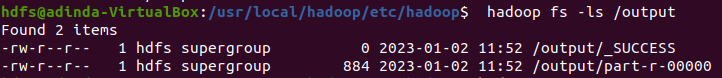
\includegraphics[width=\textwidth]{AdindaAwaliah/hasil ss no 6 wordcount}
\caption{Cek Hasil WordCount Hadoop}
\label{gam:hasil ss no 6 wordcount}
\end{figure}

\begin{figure}[!ht]
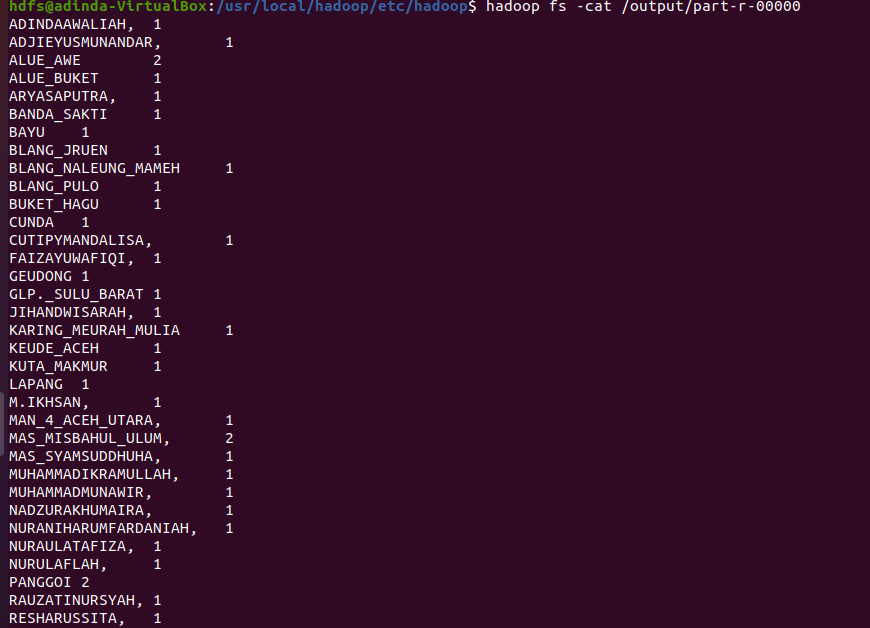
\includegraphics[width=\textwidth]{AdindaAwaliah/hasil ss no 7 wordcount}
\caption{Lihat Hasil WordCount Hadoop}
\label{gam:hasil ss no 7 wordcount}
\end{figure}

\end{enumerate}

\newday{\textbf{16 desember 2022}- Program WordCount dengan Java }
\begin{enumerate}
\item Kendala dan Solusi
\newline Tidak ada kendala saat mengerjakan praktikum

\item Kesimpulan
\newline Berhasil menampiklan hasil WordCount Java

\begin{figure}[!ht]
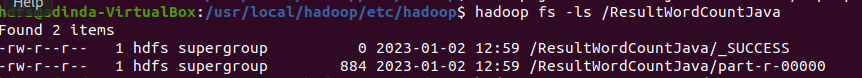
\includegraphics[width=\textwidth]{AdindaAwaliah/hasil ss no 9 wordcount java}
\caption{Cek hasil WordCount Java}
\label{gam:hasil ss no 9 wordcount java}
\end{figure}

\begin{figure}[!ht]
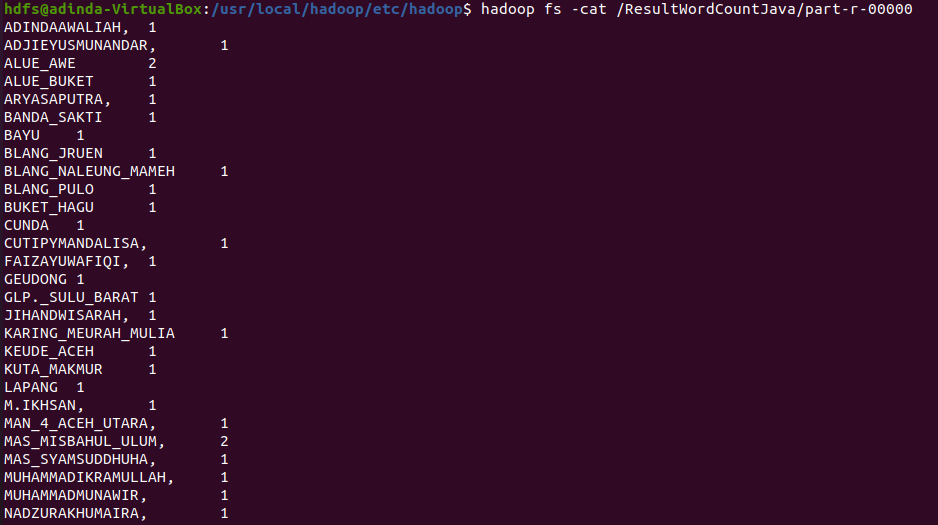
\includegraphics[width=\textwidth]{AdindaAwaliah/hasil ss no 10 wordcount java}
\caption{Lihat hasil WordCount Java}
\label{gam:hasil ss no 9 wordcount java}
\end{figure}

\end{enumerate}

\newday{\textbf{22 desember 2022}- Instalasi ApacheSpark}
\begin{enumerate}
\item Kendala dan Solusi
\newline Saat mengerjakan praktikum ini tidak ada kendala saat mengerjakan praktikum

\item Kesimpulan
\newline Berhasil melakukan installasi

\begin{figure}[!ht]
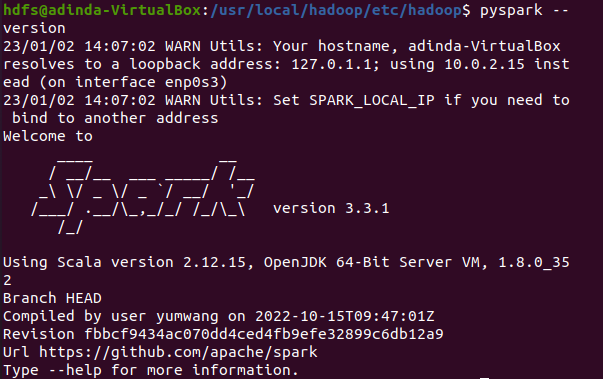
\includegraphics[width=\textwidth]{AdindaAwaliah/instalasi apache spark no 5}
\caption{Versi Spark yang terinstall}
\label{gam:instalasi apache spark no 5}
\end{figure}

\end{enumerate}

\newday{\textbf{23 desember 2022}- Program WordCount dengan Python }
\begin{enumerate}
\item Kendala dan Solusi
\newline Terkendala saat perintah menjalankan program dengan hadoop pada ~/WordCountPython/map.py -reducer tidak bisa. Solusinya  di ganti dengan /usr/local/hadoop/etc/hadoop karena sebelumnya saya sudah menjalankan program di dalam /usr/local/hadoop/etc/hadoop

\item Kesimpulan
\newline Berhasil melakukan pratikum wordcount python

\begin{figure}[!ht]
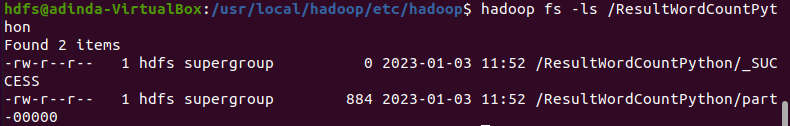
\includegraphics[width=\textwidth]{AdindaAwaliah/hasil ss no 8 wordcount python}
\caption{Cek hasil WordCount Python}
\label{gam:hasil ss no 8 wordcount python}
\end{figure}

\begin{figure}[!ht]
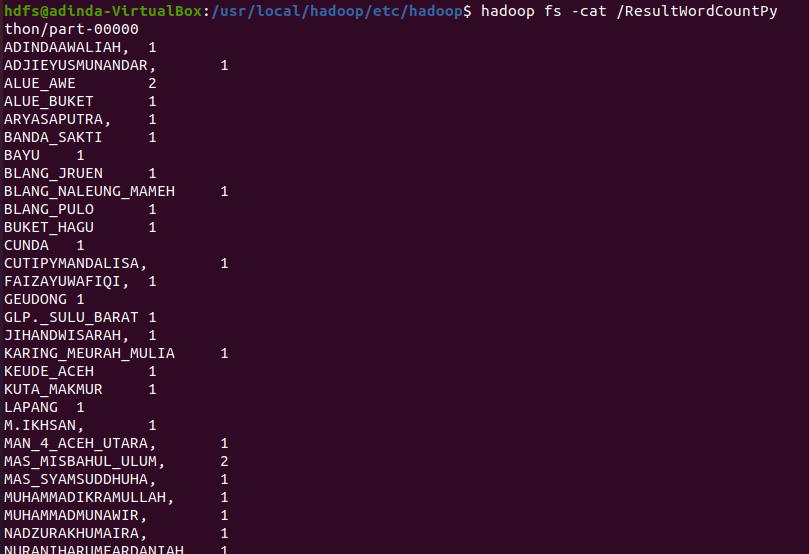
\includegraphics[width=\textwidth]{AdindaAwaliah/hasil ss no 9 wordcount python}
\caption{Lihat hasil WordCount Python}
\label{gam:hasil ss no 9 wordcount python}
\end{figure}

\end{enumerate}


\newday{\textbf{23 desember 2022}- Program WordCount dengan PySpark }
\begin{enumerate}
\item Kendala dan Solusi
\newline Saat bmengerjakan praktikum ini, tidak ditemukan kendala

\item Kesimpulan
\newline Berhasil melakukan pratikum wordcount PySpark

\begin{figure}[!ht]
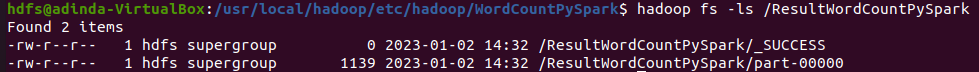
\includegraphics[width=\textwidth]{AdindaAwaliah/wordcup dengan pyspark no 6}
\caption{Cek hasil WordCount PySpark}
\label{gam:wordcup dengan pyspark no 6}
\end{figure}

\begin{figure}[!ht]
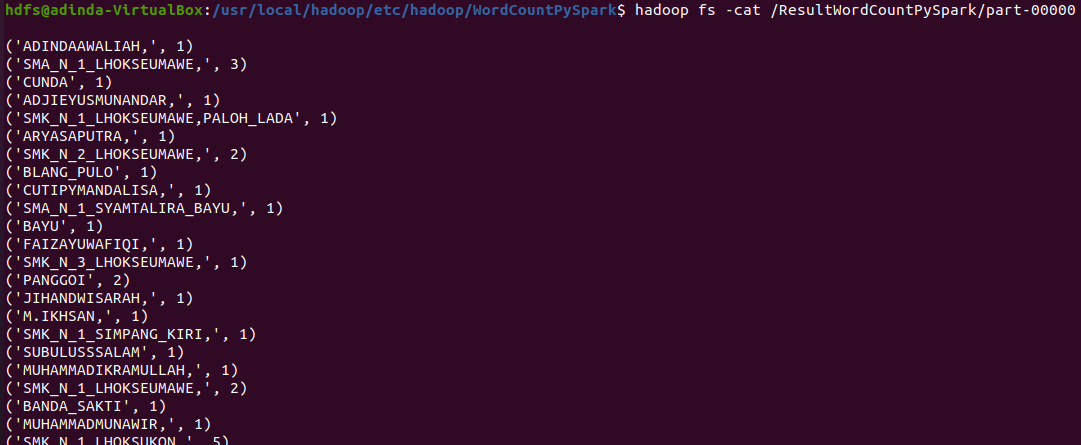
\includegraphics[width=\textwidth]{AdindaAwaliah/wordcup dengan pyspark no 7}
\caption{Lihat hasil WordCount PySprak}
\label{gam:wordcup dengan pyspark no 7}
\end{figure}

\end{enumerate}

\newday{\textbf{05 Januari 2023}- Tugas individu Program Machine Learning dengan Pyspark }
\begin{enumerate}
\item Kendala dan Solusi
\newline a. Kendala pertama pada saat menentukan nilai K 		dengan metode silhoutte, grafik tidak muncul, seharusnya setelah perintah plt.show() akan muncul grafik, belum di temukannya solusi
\newline b. Kendala selanjutnya saat menampilkan hasil Clustering dengan PCA, grafik tidak muncul, seharusnya setelah perintah plt.show() akan muncul grafik dan belum di temukannya solusi

\begin{figure}[!ht]
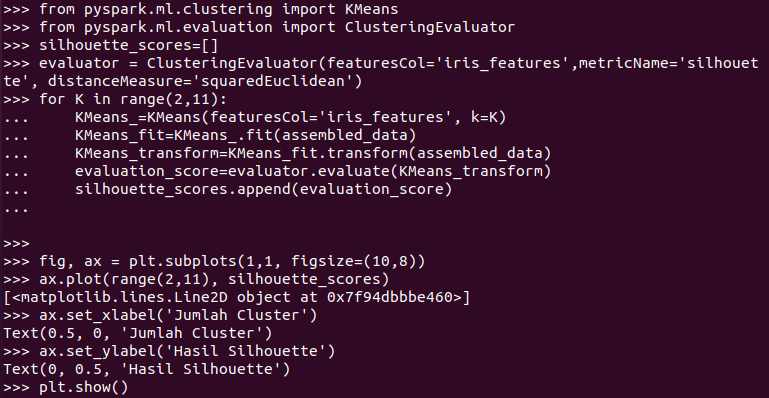
\includegraphics[width=\textwidth]{AdindaAwaliah/kendala grafik 1 nomor 5}
\caption{kendala pertama grafik tidak muncul}
\label{gam:kendala grafik 1 nomor 5}
\end{figure}


\item Kesimpulan
\newline Pada percobaan praktikum ini berhasil memunculkan tabel, namun tidak berhasil untuk memunculkan grafik. Tabel yang muncul merupakan tabel dari load data iris dan tabel penentuan nilai K asseamble data.

\begin{figure}[!ht]
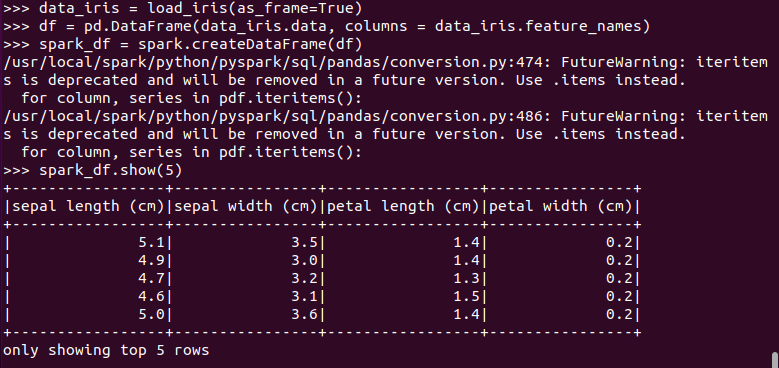
\includegraphics[width=\textwidth]{AdindaAwaliah/grafik 1}
\caption{Grafik pertama }
\label{gam:grafik 1}
\end{figure}

\begin{figure}[!ht]
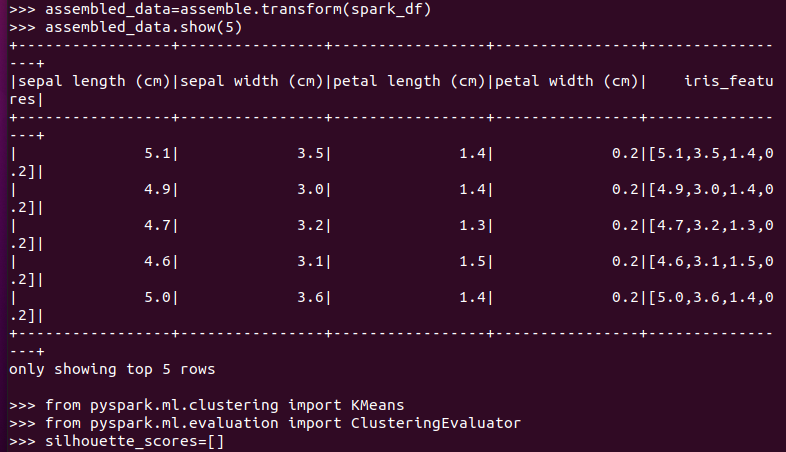
\includegraphics[width=\textwidth]{AdindaAwaliah/grafik 2}
\caption{Grafik kedua }
\label{gam:grafik 2}
\end{figure}

\end{enumerate}
\newthought{\textbf{Adjie Yusmunandar - 2020903430005 - TRKJ 3B}}

\newday{\textbf{1 - 2 Desember 2022} - Instalasi dan Konfigurasi Apache Hadoop}
\begin{enumerate}
\item Kendala dan Solusi
\begin{itemize}
\item Kendala: \\
Saat melakukan penginstalan hadoop terdapat masalah pada saat mengecek hadoop version dan  pada saat melakukan konfigurasi hadoop terdapat kendala pada saat melakukan hdfs namenode -format. Perintah ini tidak mau dijalankan karena ada kesalahan dalam penulisan pada file yarn-site.xml.

\item Solusi: \\
Melakukan perubahan penulisan pada file yarn-site.xml.
\end{itemize}

\item Kesimpulan \\
Penginstalan hadoop dan konfigurasi hadoop berhasil dijalankan sesuai perintah-perintah yang ada.

\begin{figure}
\setlength{\belowcaptionskip}{-10pt}
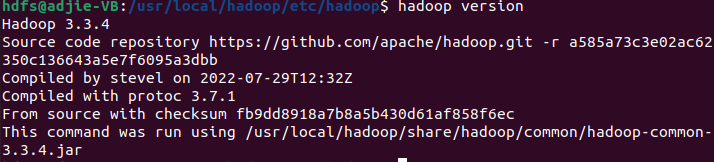
\includegraphics[width=\textwidth]{AdjieYusmunandar/instalasi hadoop}
\caption{Versi hadoop yang Terinstall}
\end{figure}

\begin{figure}
\setlength{\belowcaptionskip}{-10pt}
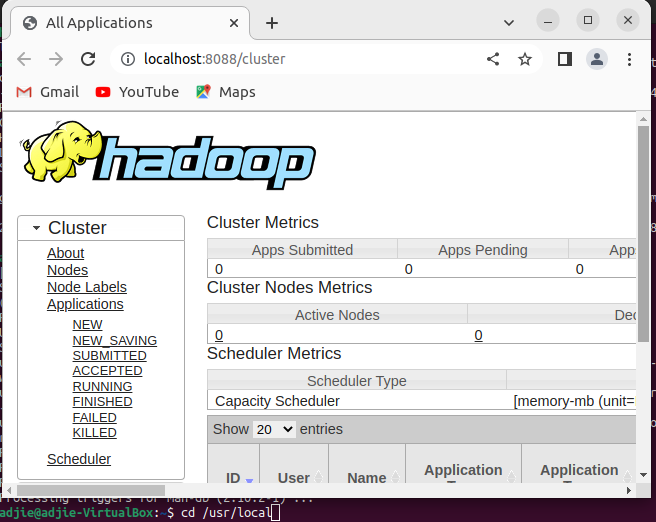
\includegraphics[width=\textwidth]{AdjieYusmunandar/Hasil dari localhost 8080}
\caption{Hasil dari localhost 8080}
\end{figure}

\begin{figure}
\setlength{\belowcaptionskip}{-10pt}
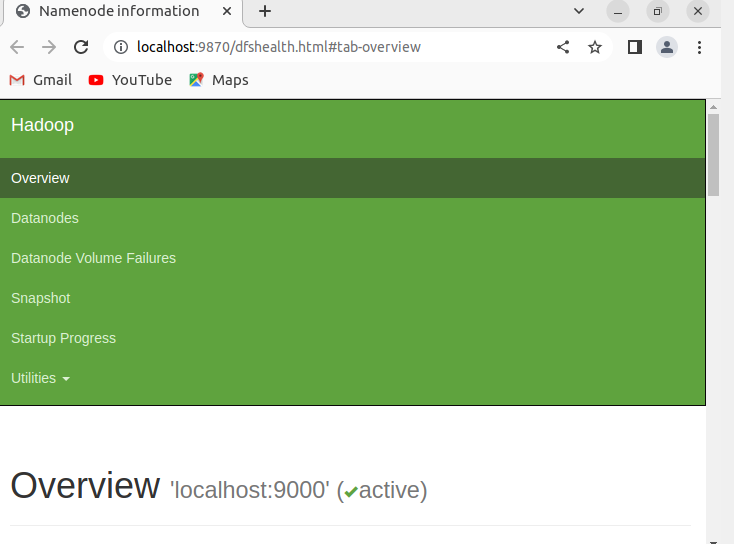
\includegraphics[width=\textwidth]{AdjieYusmunandar/Hasil dari localhost 9870}
\caption{Hasil dari localhost 9870}
\end{figure}
\end{enumerate}

\newday{\textbf{15 Desember 2022} - WordCount Bawaan Hadoop}
\begin{enumerate}
\item Kendala dan Solusi \\
Pada pertemuan hari ini, kegiatan yang dilakukan adalah mencoba program bawaan Hadoop untuk memahami bagaimana proses dan cara kerja Hadoop dalam memproses data input hingga menghasilkan sebuah output. Selama praktikum tidak mengalami kendala.

\item Kesimpulan \\
Berhasil mencoba program bawaan Hadoop yaitu program menghitung jumlah kata dalam data input yang diberikan. Berikut ini gambar bukti keberhasilan praktikum. 

\begin{figure}
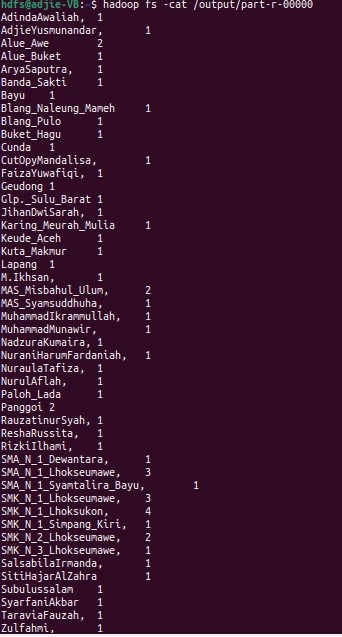
\includegraphics[width=.35\textwidth]{AdjieYusmunandar/hasill wordcount bawaan hadoop}
\caption{Output Wordcount Bawaan Hadoop}
\end{figure}

\end{enumerate}

\newday{\textbf{22 Desember 2022} - Instalasi Apache Spark (PySpark)}
\begin{enumerate}
\item Kendala dan Solusi \\
Tidak ada kendala disaat menginstall.

\item Kesimpulan\\
Berhasil melakukan instalasi apache spark (PySpark), berikut hasil praktikum :

\begin{figure}
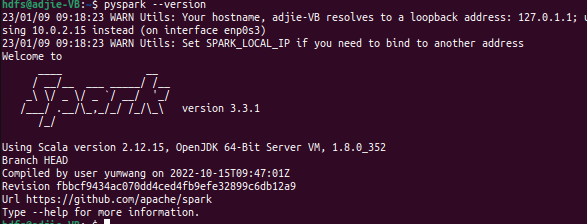
\includegraphics[width=\textwidth]{AdjieYusmunandar/Instalasi Apache Spark}
\caption{Hasil dari localhost 9870}
\end{figure}
\end{enumerate}
\newthought{\textbf{Arya Saputra - 2020903430009 - TRKJ 3B}}

\newday{\textbf{01 Desember 2022}}
\begin{enumerate}
\item Kendala dan Solusi
Pada pertemuan hari ini, kegiatan yang dilakukan adalah menginstall Apache Hadoop. Selama praktikum tidak mengalami kendala.

\item Kesimpulan
Berhasil melakukan instalasi hadoop berikut ini gambar hasil verifikasi instalasi hadoop version 

\begin{figure}[!ht]
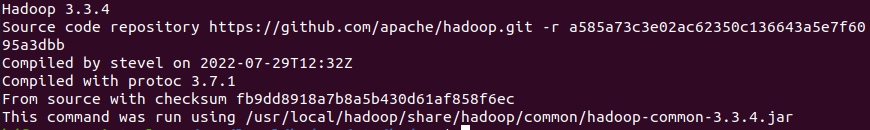
\includegraphics[width=\textwidth]{AryaSyahputra/hadoop version}
\caption{Verifikasi Hasil Instalasi Hadoop}
\label{gam:Hadoop-version}
\end{figure}
\end{enumerate}

\newday{\textbf{02 Desember 2022}}
\begin{enumerate}
\item Kendala
sudah berhasil menginstall hadoop

\item solusi
menginstal ulang ubuntu

\item Kesimpulan
setelah menginstall ulang ubuntu, instalasi dan konfigurasi hadoop berhasil

\begin{figure}[!ht]
\includegraphics[width=\textwidth]{AryaSyahputra/jps}
\caption{Verifikasi Hasil Instalasi Hadoop}
\label{gam:instalasi-hadoop}
\end{figure}
\begin{figure}[!ht]
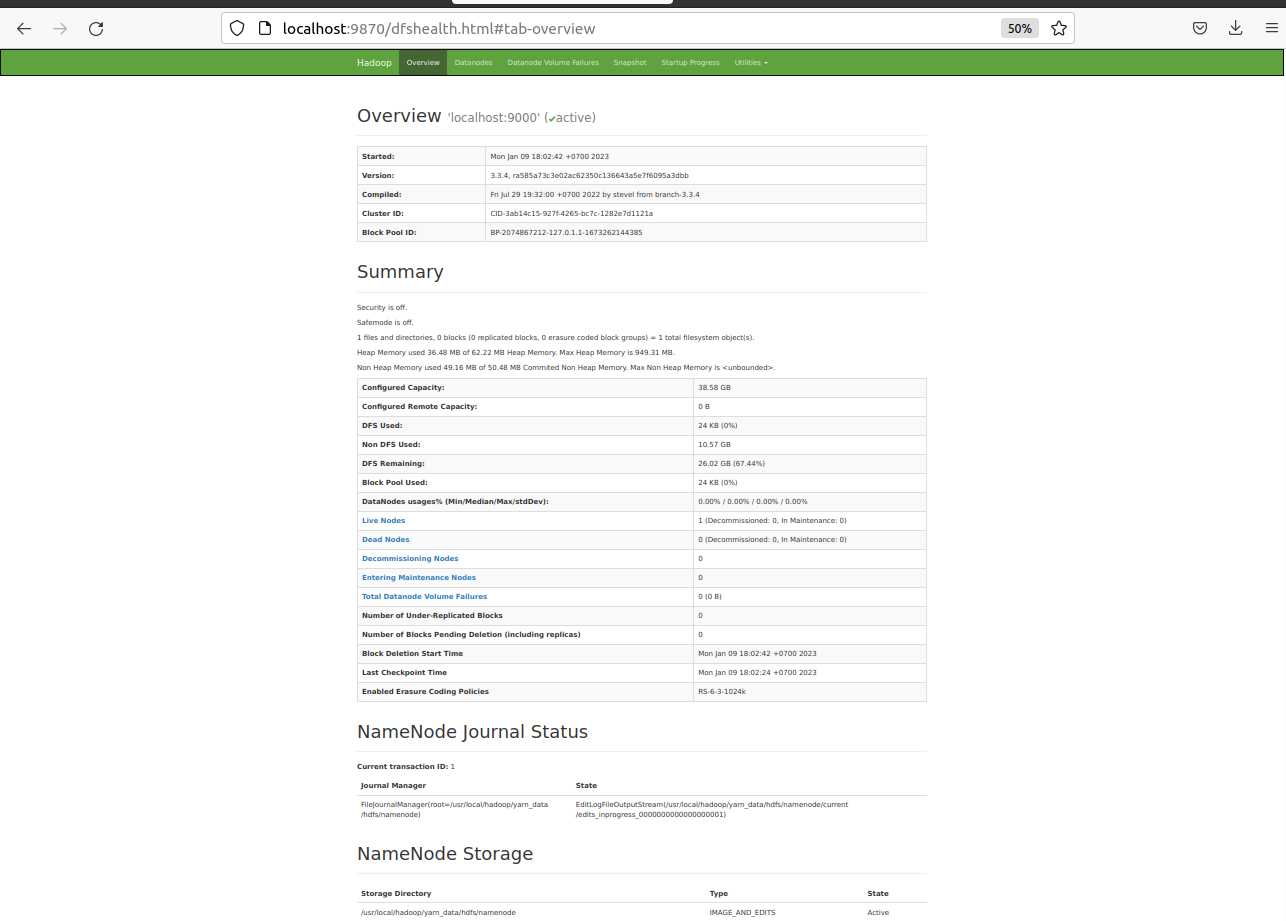
\includegraphics[width=\textwidth]{AryaSyahputra/localhos1}
\caption{Verifikasi Hasil Instalasi Hadoop}
\label{gam:instalasi-hadoop}
\end{figure}
\begin{figure}[!ht]
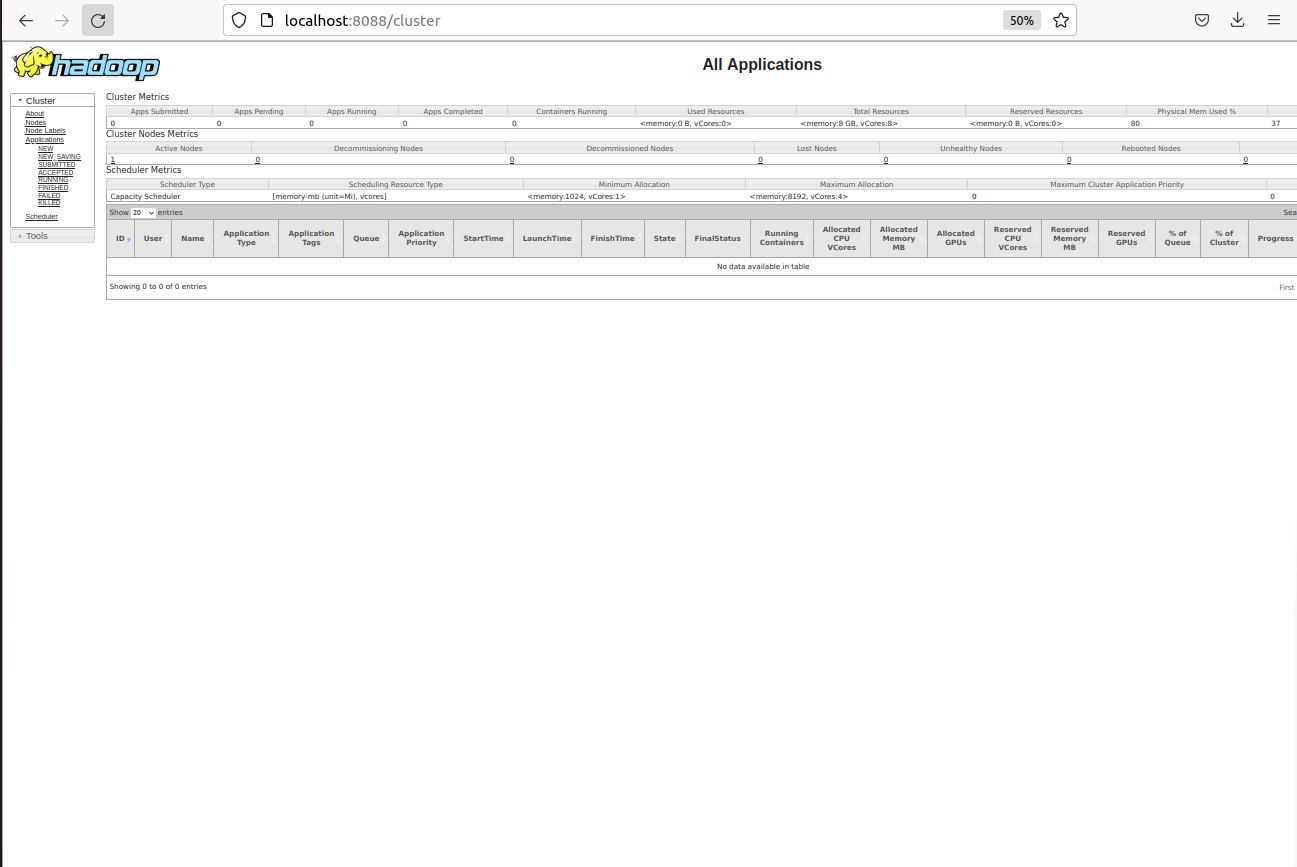
\includegraphics[width=\textwidth]{AryaSyahputra/localhos2}
\caption{Verifikasi Hasil Instalasi Hadoop}
\label{gam:instalasi-hadoop}
\end{figure}
\end{enumerate}

\clearpage
\newday{\textbf{15 Desember 2022} - WordCount Bawaan Java}
\begin{enumerate}
\item Kendala dan Solusi
\newline Tidak ada kendala apapun saat melakukan program WordCount bawaan Hadoop

\item Kesimpulan
\newline Praktikum berhasil dilakukan sesuai dengan perintah-perintah yang ada. WordCount sendiri merupakan program untuk menghitung jumlah kata yang ada pada data.


\begin{figure}[!ht]
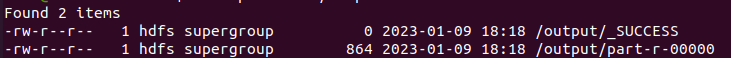
\includegraphics[width=\textwidth]{AryaSyahputra/cek hasil wordcount bawaan}
\caption{Hasil dari langkah 6}
\label{gam:wordcount bawaan}
\end{figure}
\begin{figure}[!ht]
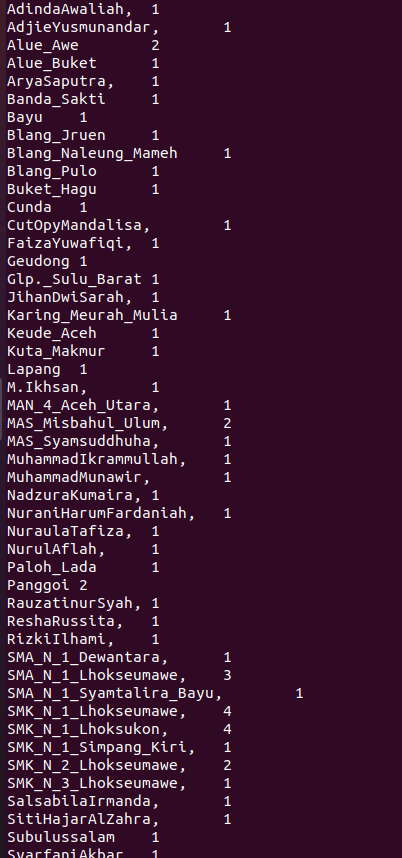
\includegraphics[width=\textwidth]{AryaSyahputra/hasil wordcount bawaan}
\caption{Hasil dari langkah 7}
\label{gam:wordcount bawaan}
\end{figure}
\begin{figure}[!ht]
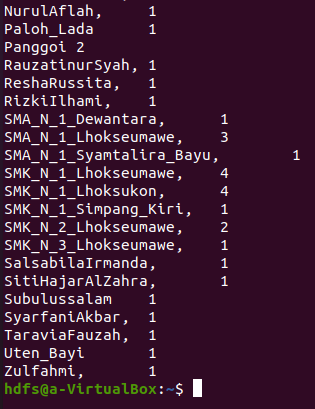
\includegraphics[width=\textwidth]{AryaSyahputra/2}
\caption{Hasil dari langkah 7}
\label{gam:wordcount bawaan}
\end{figure}
\end{enumerate}


\clearpage
\newday{\textbf{16 Desember 2022} - WordCount dengan Java}
\begin{enumerate}
\item Kendala dan Solusi
\newline Kendala :
Saat melakukan praktikum program WordCount dengan Java tidak ada kendala saat melakukan pratikum.

\item Kesimpulan
\newline Praktikum berhasil dilakukan sesuai dengan perintah-perintah yang ada. Data pada WordCount dapat ditampilkan sesuai dengan yang telah dibuat.


\begin{figure}[!ht]
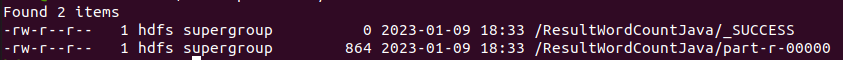
\includegraphics[width=\textwidth]{AryaSyahputra/cek hasil resultwordcountjava}
\caption{Hasil Perhitungan dengan WordCount Hadoop}
\label{gam:result wordcount java}
\end{figure}
\begin{figure}[!ht]
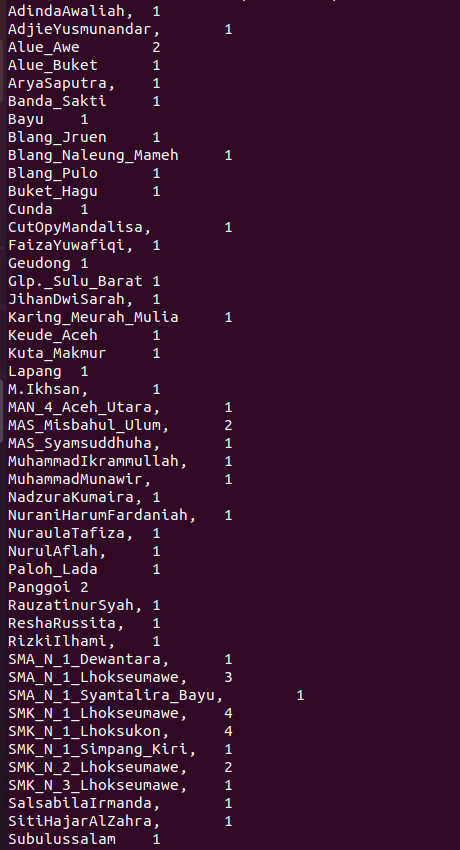
\includegraphics[width=\textwidth]{AryaSyahputra/hasil wordcount java}
\caption{Hasil Perhitungan dengan WordCount Hadoop}
\label{gam:result wordcount java}
\end{figure}
\begin{figure}[!ht]
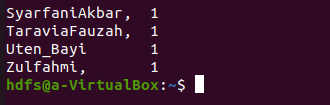
\includegraphics[width=\textwidth]{AryaSyahputra/hasil wordcount java1}
\caption{Hasil Perhitungan dengan WordCount Hadoop}
\label{gam:result wordcount java}
\end{figure}

\end{enumerate}


\clearpage
\newday{\textbf{22 Desember 2022}- Instalasi Apache Spark (PySpark)}
\begin{enumerate}
\item Kendala dan Solusi
\newline Kendala :\\
Saat melakukan praktikum instalasi apache spark tidak ada kendala saat melakukan pratikum.

\item Kesimpulan
\newline Proses penginstalan Apache Spark berhasil dilakukan tanpa adanya kendala satupun


\begin{figure}[!ht]
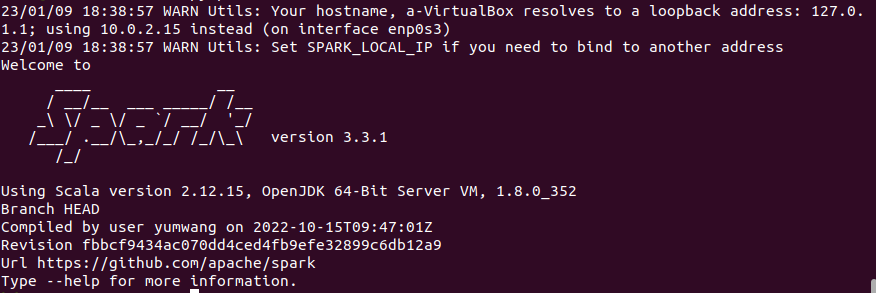
\includegraphics[width=\textwidth]{AryaSyahputra/spark}
\caption{Hasil instalasi apache spark}
\label{gam:instalasi apache spark}
\end{figure}
\end{enumerate}


\clearpage
\newday{\textbf{23 Desember 2022}- Program WordCount dengan Python}
\begin{enumerate}
\item Kendala dan Solusi
\newline Kendala :\\
tidak ada kendala saat melakukan pratikum resultwordcountpython.

\item Kesimpulan
\newline setelah melakukan percobaan dari tahap awal sampai selesai, kemudian melakukan pengecekan hasil dan melihat hasil word count dengan python. jika hasilnya muncul dan sesuai maka pratikan telah berhasil melakukan percobaan word count dengan python.


\begin{figure}[!ht]
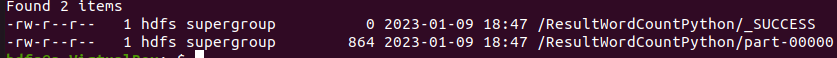
\includegraphics[width=\textwidth]{AryaSyahputra/cek hasil resultwordcountpython}
\caption{Hasil wordcountpython}
\label{gam:wordcountpython}
\end{figure}
\begin{figure}[!ht]
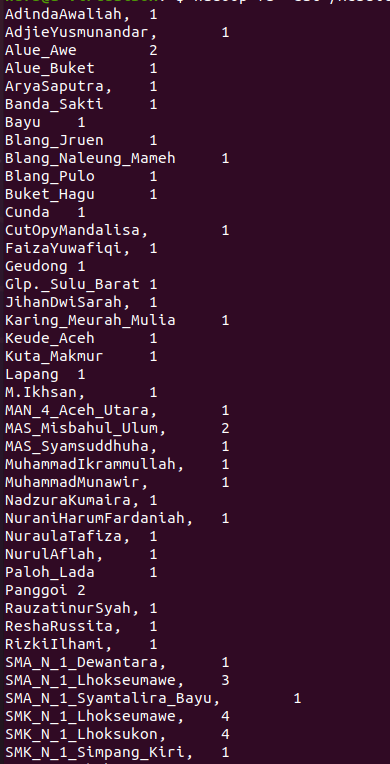
\includegraphics[width=\textwidth]{AryaSyahputra/hasil result wordcount python}
\caption{Hasil wordcountpython}
\label{gam:wordcountpython}
\end{figure}
\begin{figure}[!ht]
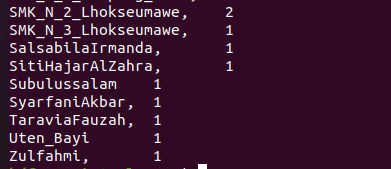
\includegraphics[width=\textwidth]{AryaSyahputra/hasil result wordcount python1}
\caption{Hasil wordcountpython}
\label{gam:wordcountpython}
\end{figure}
\end{enumerate}


\clearpage
\newday{\textbf{02 Januari 2023} Wordcountpyspark}
\begin{enumerate}
\item Kendala dan Solusi
\newline Kendala :\\
tidak ada kendala saat melakukan pratikum.

\item Kesimpulan
\newline Berhasil menjalankan program wordcountpyspark.


\begin{figure}[!ht]
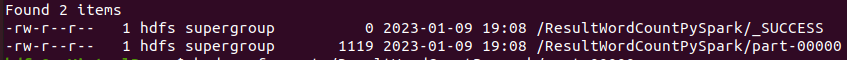
\includegraphics[width=\textwidth]{AryaSyahputra/cek hasil rasultwordcountpyspark}
\caption{Hasil resultwordcountpyspark}
\label{gam:resultwordcountpyspark}
\end{figure}

\begin{figure}[!ht]
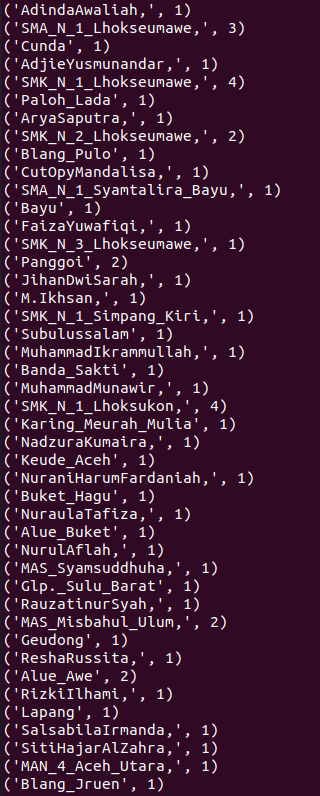
\includegraphics[width=\textwidth]{AryaSyahputra/hasil resultwordcountpyspark}
\caption{Hasil resultwordcountpyspark}
\label{gam:resultwordcountpyspark}
\end{figure}

\begin{figure}[!ht]
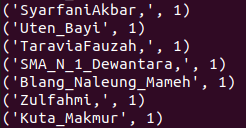
\includegraphics[width=\textwidth]{AryaSyahputra/hasil resultwordcountpyspark1}
\caption{Hasil resultwordcountpyspark}
\label{gam:resultwordcountpyspark}
\end{figure}
\end{enumerate}

\newthought{\textbf{Cut Opy Mandalisa - 2020903430012 - TRKJ 3B}}

\newday{\textbf{1-2 Desember 2022- Instalasi dan Konfigurasi Hadoop}}
\begin{enumerate}
\item Kendala dan Solusi\\
% jelaskan kendala dan penyebab yang dialami saat mengikuti praktikum serta solusi atau langkah-langkah yang telah dilakukan
Pada Praktikum pertama yaitu penginstalan apache hadoop.kendala yang didapat tidak bisa membuka firefox kemudian solusinya dengan menginstal firefox baru.

\begin{figure}[!ht]
\includegraphics[width=\textwidth]{CutOpyMandalisa/01}
\caption{hasil dari cek hadoop service}
\label{gam:perkuliahan-25-11}
\end{figure}

\begin{figure}[!ht]
\includegraphics[width=\textwidth]{CutOpyMandalisa/02}
\caption{hasil cek hadoop service}
\label{gam:perkuliahan-25-11}
\end{figure}

\item Kesimpulan\\
% berikan kesimpulan dari praktikum yang telah dikerjkan
Behasil mendownload dan menginstal Apache hadoop dan sudah bisa dijalankan
\end{enumerate}


\newday{\textbf{08 Desember 2022-WordCount bawaan Hadoop}}
\begin{enumerate}

\item Kendala dan Solusi
\newpage
% jelaskan kendala dan penyebab yang dialami saat mengikuti praktikum serta solusi atau langkah-langkah yang telah dilakukan
Pada praktikum ini membuat program WordCount bawaan Hadoop. Pada melakukan praktikum tidak ada kendala hanya erorr dikarenakan salah memasukkan perintah.

\begin{figure}[!ht]
\includegraphics[width=\textwidth]{CutOpyMandalisa/03}
\caption{hasil WordCount bawaan Hadoop}
\label{gam:perkuliahan-25-11}
\end{figure}

\item Kesimpulan\\
% berikan kesimpulan dari praktikum yang telah dikerjkan
Pada praktikum ini untuk memahami proses cara kerja pada hadoop dalam memproses data input sehingga menghasilkan output.Wordcount merupakan program untuk menghitung jumlah kata dalam input.
\end{enumerate}


\newday{\textbf{09 Desember 2022-WordCount dengan Java}}
\begin{enumerate}
\item Kendala dan Solusi\\
% jelaskan kendala dan penyebab yang dialami saat mengikuti praktikum serta solusi atau langkah-langkah yang telah dilakukan
Pada praktikum ini membuat program WordCount dengan java.Pada saat melakukan praktikum terdapat error akan tetapi erorrnya disebabkan salah memasukkan perintah codingannya.solusinya harus lebih teliti saat memasukkan codingan tersebut.

\begin{figure}[!ht]
\includegraphics[width=\textwidth]{CutOpyMandalisa/04}
\caption{hasil wordCount dengan java}
\label{gam:perkuliahan-25-11}
\end{figure}

\item Kesimpulan\\
% berikan kesimpulan dari praktikum yang telah dikerjkan
Berhasil menjalankan program WordCount dengan java.
\end{enumerate}


\newday{\textbf{15 Desember 2022}}
\begin{enumerate}
\item Kendala dan Solusi
% jelaskan kendala dan penyebab yang dialami saat mengikuti praktikum serta solusi atau langkah-langkah yang telah dilakukan

\item Kesimpulan
% berikan kesimpulan dari praktikum yang telah dikerjkan
\end{enumerate}


\newday{\textbf{16 Desember 2022}}
\begin{enumerate}
\item Kendala dan Solusi
% jelaskan kendala dan penyebab yang dialami saat mengikuti praktikum serta solusi atau langkah-langkah yang telah dilakukan

\item Kesimpulan
% berikan kesimpulan dari praktikum yang telah dikerjkan
\end{enumerate}

\newday{\textbf{22 Desember 2022}}
\begin{enumerate}
\item Kendala dan Solusi
% jelaskan kendala dan penyebab yang dialami saat mengikuti praktikum serta solusi atau langkah-langkah yang telah dilakukan

\item Kesimpulan
% berikan kesimpulan dari praktikum yang telah dikerjkan
\end{enumerate}

\newday{\textbf{23 Desember 2022}}
\begin{enumerate}
\item Kendala dan Solusi
% jelaskan kendala dan penyebab yang dialami saat mengikuti praktikum serta solusi atau langkah-langkah yang telah dilakukan

\item Kesimpulan
% berikan kesimpulan dari praktikum yang telah dikerjkan
\end{enumerate}
\newthought{\textbf{Faiza Yuwafiqi - 2020903430014 - TRKJ 3B}}

\newday{\textbf{1-2 Desember 2022} - Instalasi dan Konfigurasi Apache Hadoop}

\begin{enumerate}
\item Kendala dan Solusi
\newline Pada saat penginstalan dan konfigurasi hadoop tidak ada kendala apapun.

\item Kesimpulan
\newline instalasi dan konfigurasi hadoop berhasil dilakukan

\begin{figure}
\includegraphics[width=\textwidth]
{FaizaYuwafiqi/jps}
\caption{hasil dari jps}
\label{gam:perkuliahan-25-11}
\end{figure}

\begin{figure}
\includegraphics[width=\textwidth]
{FaizaYuwafiqi/localhost9870}
\caption{hasil dari localhost 9870}
\label{gam:perkuliahan-25-11}
\end{figure}

\newpage
\begin{figure}
\includegraphics[width=\textwidth]
{FaizaYuwafiqi/localhost8088}

\caption{hasil dari localhost 8088}
\label{gam:perkuliahan-25-11}
\end{figure}

\end{enumerate}


\newday{\textbf{8 Desember 2022}}
\begin{enumerate}
\item Kendala dan Solusi
% jelaskan kendala dan penyebab yang dialami saat mengikuti praktikum serta solusi atau langkah-langkah yang telah dilakukan

\item Kesimpulan
% berikan kesimpulan dari praktikum yang telah dikerjkan

\end{enumerate}

\newday{\textbf{9 Desember 2022}}
\begin{enumerate}
\item Kendala dan Solusi
% jelaskan kendala dan penyebab yang dialami saat mengikuti praktikum serta solusi atau langkah-langkah yang telah dilakukan

\item Kesimpulan
% berikan kesimpulan dari praktikum yang telah dikerjkan

\end{enumerate}

\newday{\textbf{15 Desember 2022}- WordCount Bawaan Hadoop}
\begin{enumerate}
\item Kendala dan Solusi
\newline Kendala, masalahnya saat pengisian nano ada yang typo sehingga program lain tidak mau jalan.
\newline Solusi, memperbaiki typo pada nano dan program berhasil jalan

\item Kesimpulan
\newline harus lebih memperhatikan codingan yang diketik agar tidak terjadi typo dan program tidak mau jalan

\newpage
\begin{figure}
\includegraphics[width=\textwidth]
{FaizaYuwafiqi/6 dan 7 a}
\caption{hasil dari langkah 6 dan 7}
\label{gam:perkuliahan-25-11}
\end{figure}

\begin{figure}
\includegraphics[width=\textwidth]
{FaizaYuwafiqi/6 dan 7 b}
\caption{sambungan hasil dari langkah 7}
\label{gam:perkuliahan-25-11}
\end{figure}

\end{enumerate}

\newday{\textbf{16 Desember 2022} -WordCount dengan Java}
\begin{enumerate}
\item Kendala dan Solusi
\newline Kendala, program tidak mau di compile karna ada penulisan yang typo dan tertinggal dalam nano.
\newline Solusi, memperbaiki isi nano

\item Kesimpulan
\newline beberapa kesalahan terjadi karena isi modul yang berubah, sehingga harus mencari modul lama yang memiliki codingan lengkap.

\newpage
\begin{figure}
\includegraphics[width=\textwidth]
{FaizaYuwafiqi/9 dan 10 a}
\caption{hasil dari langkah 9 dan 10}
\label{gam:perkuliahan-25-11}
\end{figure}

\begin{figure}
\includegraphics[width=\textwidth]
{FaizaYuwafiqi/10 b}
\caption{sambungan hasil dari langkah 10}
\label{gam:perkuliahan-25-11}
\end{figure}

\end{enumerate}

\newday{\textbf{22 Desember 2022}}
\begin{enumerate}
\item Kendala dan Solusi
\newline Pada saat melakukan instalasi tidak ada terjadi error

\item Kesimpulan
\newline instalasi berjalan lancar

\newpage
\begin{figure}
\includegraphics[width=\textwidth]
{FaizaYuwafiqi/pyspark}
\caption{hasil dari instalasi pyspark}
\label{gam:perkuliahan-25-11}
\end{figure}

\end{enumerate}

\newday{\textbf{23 Desember 2022}}
\begin{enumerate}
\item Kendala dan Solusi
pada saat proses wordcount dilakukan terdapat typo pada penulisan kata WordCount sehingga nano tidak tersimpan dengan benar

\item Kesimpulan
kesalahan tersebut telah diperbaiki

\newpage
\begin{figure}
\includegraphics[width=\textwidth]
{FaizaYuwafiqi/wc pyspark}
\caption{hasil dari Wordcount Pyspark}
\label{gam:perkuliahan-25-11}
\end{figure}

\begin{figure}
\includegraphics[width=\textwidth]
{FaizaYuwafiqi/wc pyspark 2}
\caption{sambungan hasil dari Wordcount Pyspark 2}
\label{gam:perkuliahan-25-11}
\end{figure}

\end{enumerate}


\newthought{\textbf{Jihan Dwi Sarah - 2020903430015 - TRKJ 3B}}


\newday{\textbf{1 - 2 Desember 2022} - Instalasi Hadoop}
\begin{enumerate}
\item Kendala dan Solusi
% jelaskan kendala dan penyebab yang dialami saat mengikuti praktikum serta solusi atau langkah-langkah yang telah dilakukan
\newline Pada pertemuan hari ini, kegiatan yang dilakukan adalah menginstall Apache Hadoop. Selama praktikum tidak mengalami kendala.

\item Kesimpulan \\
% berikan kesimpulan dari praktikum yang telah dikerjkan
Berhasil melakukan instalasi java tanpa ada bug atau error serta instalasi hadoop berikut ini gambar hasil verifikasi instalasi java version dan hadoop version 

\begin{figure}[!ht]
\includegraphics[width=\textwidth]{JihanDwiSarah/Java-version(Jihan)}
\caption{Verifikasi Hasil Instalasi Java}
\label{gam:Java-version(Jihan)}
\end{figure} 

\begin{figure}[!ht]
\includegraphics[width=\textwidth]{JihanDwiSarah/Hadoop-version(Jihan)}
\caption{Verifikasi Hasil Instalasi Hadoop}
\label{gam:Hadoop-version(Jihan)}
\end{figure}
\end{enumerate}


\newday{\textbf{8 - 9 Desember 2022} - Konfigurasi Hadoop}
\begin{enumerate}
\item Kendala dan Solusi \\
% jelaskan kendala dan penyebab yang dialami saat mengikuti praktikum serta solusi atau langkah-langkah yang telah dilakukan
Pada pertemuan hari ini, kegiatan yang dilakukan adalah mengkonfigurasi Apache Hadoop. Selama praktikum tidak mengalami kendala.

\item Kesimpulan \\
% berikan kesimpulan dari praktikum yang telah dikerjkan
Berhasil mengkonfigurasi beberapa file Hadoop sehingga memudahkan dalam memonitoring ekosistem Hadoop yang telah diinstall. Berikut ini gambar bukti keberhasilan praktikum. 

\begin{figure}[!ht]
\includegraphics[width=\textwidth]{JihanDwiSarah/perintah-jps(jihan)}
\caption{Hasil perintah jps}
\label{gam:perintah-jps(jihan)}
\end{figure} 


\begin{figure}[!ht]
\includegraphics[width=\textwidth]{JihanDwiSarah/Akses-web-browser-8088(Jihan)}
\caption{Akses melalui web browser dengan alamat http://localhost:8088}
\label{gam:Akses-web-browser-8088(Jihan)}
\end{figure} 

\begin{figure}[!ht]
\includegraphics[width=\textwidth]{JihanDwiSarah/Akses-web-browser-9870(Jihan)}
\caption{Akses melalui web browser dengan alamat http://localhost:9870}
\label{gam:Akses-web-browser-9870(Jihan)}
\end{figure} 
\end{enumerate}

\newday{\textbf{15 Desember 2022} - WordCount Bawaan Hadoop}
\begin{enumerate}
\item Kendala dan Solusi \\
% jelaskan kendala dan penyebab yang dialami saat mengikuti praktikum serta solusi atau langkah-langkah yang telah dilakukan
Pada pertemuan hari ini, kegiatan yang dilakukan adalah mencoba program bawaan Hadoop untuk memahami bagaimana
proses dan cara kerja Hadoop dalam memproses data input hingga menghasilkan sebuah output. Selama praktikum tidak mengalami kendala.

\item Kesimpulan\\
% berikan kesimpulan dari praktikum yang telah dikerjkan
Berhasil mencoba program bawaan Hadoop yaitu program menghitung jumlah kata dalam data input yang diberikan.Berikut ini gambar bukti keberhasilan praktikum. 
\begin{figure}[!ht]
\includegraphics[width=\textwidth]{JihanDwiSarah/WordCount bawaan-Hadoop(jihan)}
\caption{Output Wordcount Bawaan Hadoop}
\label{gam:WordCount bawaan-Hadoop(jihan)}
\end{figure}
\end{enumerate}

\newday{\textbf{16 Desember 2022} - Program WordCount dengan Java}
\begin{enumerate}
\item Kendala dan Solusi 
% jelaskan kendala dan penyebab yang dialami saat mengikuti praktikum serta solusi atau langkah-langkah yang telah dilakukan
Pada pertemuan hari ini, kegiatan yang dilakukan adalah mencoba program  wordcount dengan java. Selama praktikum mengalami kendala pada poin ke-6 berdasarkan urutan di modul. Program tidak mau dicompile karena kesalahan penulisan perintah.\\

solusinya adalah menggunakan perintah seperti berikut 
\begin{figure}[!ht]
\includegraphics[width=\textwidth]{JihanDwiSarah/solusi-java-compile(jihan)}
\caption{Solusi Meng-Compile java}
\label{gam:solusi-java-compile(jihan)}
\end{figure}


\item Kesimpulan\\
% berikan kesimpulan dari praktikum yang telah dikerjkan
Dapat memberikan pemahaman mengenai proses membuat program wordcount java, menyiapkan data, meng-compile program hingga menjalankan program dan memperoleh hasilnya. Berikut hasil praktikum.

\begin{figure}[!ht]
\includegraphics[width=\textwidth]{JihanDwiSarah/WordCount-Java(jihan)}
\caption{Output Wordcount java}
\label{gam:WordCount-Java(jihan)}
\end{figure}
\end{enumerate}

\newday{\textbf{17 Desember 2022} - Instalasi Apache Spark (PySpark)}
\begin{enumerate}
\item Kendala dan Solusi \\
% jelaskan kendala dan penyebab yang dialami saat mengikuti praktikum serta solusi atau langkah-langkah yang telah dilakukan
Terdapat kendala pada poin ke 3 karena kesalahan dari modulnya, perintah yang benar adalah sebagai berikut:\\
sudo mv spark-3.3.1-bin-hadoop3.\\
tidak perlu menambahkan '/usr/local/spark' lagi di akhir.


\item Kesimpulan\\
% berikan kesimpulan dari praktikum yang telah dikerjkan
Berhasil melakukan instalasi apache spark (PySpark), berikut hasil praktikum : \\

\begin{figure}[!ht]
\includegraphics[width=\textwidth]{JihanDwiSarah/Instalasi-Spark(jihan)}
\caption{Hasil Instalasi Spark}
\label{gam:Instalasi-Spark(jihan)}
\end{figure}


\end{enumerate}


\newday{\textbf{22 Desember 2022} - Program WordCount dengan Python }
\begin{enumerate}
\item Kendala dan Solusi \\
% jelaskan kendala dan penyebab yang dialami saat mengikuti praktikum serta solusi atau langkah-langkah yang telah dilakukan
Terdapat error di poin ke-6 yaitu mencoba program local. Belum ada solusinya 

\item Kesimpulan\\
% berikan kesimpulan dari praktikum yang telah dikerjkan
Belum ada hasil akhir, karena masih ada kendala. Masih mencoba sampai berhasil.
\begin{figure}[!ht]
\includegraphics[width=\textwidth]{JihanDwiSarah/kendala-WordCountPython(jihan)}
\caption{Kendala Program Local}
\label{gam:kendala-WordCountPython(jihan)}
\end{figure}


\end{enumerate}

\newday{\textbf{23 Desember 2022} - Program WordCount dengan Pyspark }
\begin{enumerate}
\item Kendala dan Solusi \\
% jelaskan kendala dan penyebab yang dialami saat mengikuti praktikum serta solusi atau langkah-langkah yang telah dilakukan
Pada pertemuan hari ini, kegiatan yang dilakukan adalah mencoba program  wordcount dengan Pyspark. Selama praktikum tidak mengalami kendala.

\item Kesimpulan\\
% berikan kesimpulan dari praktikum yang telah dikerjkan
Berhasil menjalankan program menggunakan PySpark, berikut hasil yang diperoleh \\

\begin{figure}[!ht]
\includegraphics[width=\textwidth]{JihanDwiSarah/WordCount-PySpark(jihan)}
\caption{Output Wordcount PySpark}
\label{gam:WordCount-PySpark(jihan)}
\end{figure}
\end{enumerate}

\newday{\textbf{25 Desember 2022} - Program WordCount dengan Python }
\begin{enumerate}
\item Kendala dan Solusi \\
% jelaskan kendala dan penyebab yang dialami saat mengikuti praktikum serta solusi atau langkah-langkah yang telah dilakukan
Kendala yang  pertama terdapat di poin ke-6 yaitu mencoba program local. Solusinya adalah menambahkan python3 di dalam program map.py dan reduce.py karena versi python yang tersedia adalah python3, baru setelah itu program di lokal bisa di jalankan. berikut program yang benar : \\
\begin{figure}[!ht]
\includegraphics[width=\textwidth]{JihanDwiSarah/solusi-python-poin-6(jihan)}
\caption{solusi python poin 6}
\label{gam:solusi-python-poin-6(jihan)}
\end{figure} 

kendala yang kedua tidak bisa menjalankan program hadoop python. Terdapat pesan error 'Streaming Command Failed' seperti gambar di bawah ini :
\begin{figure}[!ht]
\includegraphics[width=\textwidth]{JihanDwiSarah/kendala-menjalankan-hadoop-python(jihan)}
\caption{Kendala Menjalankan Hadoop Python}
\label{gam:kendala-menjalankan-hadoop-python(jihan)}
\end{figure} 

Ternyata kesalahannya adalah saya tidak mendeklarasikan direktori penyimpanan program WordCountPython dengan benar. Saya menyimpan program WordCountPython di dalam direktori '/usr/local/hadoop/etc/hadoop'. jadi saya harus mendeklasikan direktori tersebut terlebih dahulu, baru setelah itu program hadoop python ini bisa dijalankan. berikut perintah yang benar.
\begin{figure}[!ht]
\includegraphics[width=\textwidth]{JihanDwiSarah/solusi-python(jihan)}
\caption{Solusi Menjalankan hadoop Python(jihan)}
\label{gam:solusi-python(jihan)}
\end{figure} 

\item Kesimpulan\\
% berikan kesimpulan dari praktikum yang telah dikerjkan
Berhasil menjalankan program wordcount dengan python walaupun banyak mengalami kendala, berikut bukti hasil praktikum. 

\begin{figure}[!ht]
\includegraphics[width=\textwidth]{JihanDwiSarah/program-local-python(jihan)}
\caption{Mencoba program di local}
\label{gam:program-local-python(jihan)}
\end{figure} 

\begin{figure}[!ht]
\includegraphics[width=\textwidth]{JihanDwiSarah/WordCount-Python(jihan)}
\caption{Hasil wordcount python}
\label{gam:WordCount-Python(jihan)}
\end{figure} 



\begin{figure}[!ht]
\includegraphics[width=\textwidth]{JihanDwiSarah/WordCount-Python2(jihan)}
\caption{Hasil wordcount python2}
\label{gam:WordCount-Python2(jihan)}
\end{figure} 

\end{enumerate}

\newday{\textbf{31 Desember 2022} - Program Machine Learning dengan PySpark (Individu)}

\begin{enumerate}
\item Kendala dan Solusi \\
% jelaskan kendala dan penyebab yang dialami saat mengikuti praktikum serta solusi atau langkah-langkah yang telah dilakukan
Banyak mengalami kendala karena tidak paham awalnya. Selain itu, banyak program yang error karena kesalahan dari penulisan program. Terjadi error pada poin ke-5 yaitu menentukan nilai K dengan metode silhouette yaitu setelah program 'for K in range (2,11)'. Solusinya adalah dengan mengetikkan tab, baru setelah itu dilanjutkan dengan menulis program sampai selesai.

\item Kesimpulan  \\
% berikan kesimpulan dari praktikum yang telah dikerjkan
Berhasil menjalankan Program Machine Learning dengan PySpark pada awalnya banyak mengalami kendala. Berikut ini gambar sebagai bukti praktikum : 
\end{enumerate}
\begin{figure}[!ht]
\includegraphics[width=\textwidth]{JihanDwiSarah/Spark-df-show(jihan)}
\caption{Hasil Spark df show}
\label{gam:Spark-df-show(jihan)}
\end{figure}

\begin{figure}[!ht]
\includegraphics[width=\textwidth]{JihanDwiSarah/assembled-data-show(jihan)}
\caption{Hasil assembled-data-show}
\label{gam:assembled-data-show(jihan)}
\end{figure}

\newpage
\begin{figure}[!ht]
\includegraphics[width=\textwidth]{JihanDwiSarah/Menentukan-nilai-K-dengan-silhouette(jihan)}
\caption{Menentukan Nilai-K Dengan Silhouette}
\label{gam:Menentukan-nilai-K-dengan-silhouette(jihan)}
\end{figure}

\begin{figure}[!ht]
\includegraphics[width=\textwidth]{JihanDwiSarah/Hasil-clustering-dengan-PCA(jihan)}
\caption{Hasil Clustering Dengan PCA}
\label{gam:Hasil-clustering-dengan-PCA(jihan)}
\end{figure}


\newday{\textbf{31 Desember 2022} - Tugas Kelompok 1}
\begin{enumerate}
\item Kendala dan Solusi
% jelaskan kendala dan penyebab yang dialami saat mengikuti praktikum serta solusi atau langkah-langkah yang telah dilakukan
\newline kendalanya terdapat error ketika menjalankan perintah menggunakan spark-submit. pesan errornya adalah 'NameError : name 'spark' is not defined'.
\begin{figure}[!ht]
\includegraphics[width=\textwidth]{TugasKelompok/Kelompok1/kendala}
\caption{Kendala menjalankan spark-submit}
\label{gam:kendala}
\end{figure} 
\newpage
solusinya adalah mengimport beberapa modul berikut :
\begin{figure}[!ht]
\includegraphics[width=\textwidth]{TugasKelompok/Kelompok1/solusi}
\caption{solusi menjalankan spark-submit}
\label{gam:solusi}
\end{figure} 

\item Kesimpulan \\
% berikan kesimpulan dari praktikum yang telah dikerjkan
Berhasil menyelesaikan tugas kelompok yaitu membuat program dalam bentuk file Python sehingga
dapat dijalankan menggunakan spark-submit.

berikut ini langkah-langkah praktikum :\\
a. Membuat direktori dengan nama ruangPyspark, lalu di dalam direktori tersebut membuat file python bernama progpyspark.py
\begin{figure}[!ht]
\includegraphics[width=\textwidth]{TugasKelompok/Kelompok1/membuat-direktori}
\caption{Membuat direktori baru}
\label{gam:membuat-direktori}
\end{figure} 


b. Membuat program berikut ini di dalam file python bernama progpyspark.py
\begin{figure}[!ht]
\includegraphics[width=\textwidth]{TugasKelompok/Kelompok1/prog1_1}
\caption{Program python}
\label{gam:prog1_1}
\end{figure} 

\newpage
\begin{figure}[!ht]
\includegraphics[width=\textwidth]{TugasKelompok/Kelompok1/prog1_2}
\caption{Program python}
\label{gam:prog1_2}
\end{figure}


c. Menjalankan Program menggunakan PySpark. Prosesnya sedikit lama, tunggu sampai selesai
\begin{figure}[!ht]
\includegraphics[width=\textwidth]{TugasKelompok/Kelompok1/perintah-spark-submit}
\caption{Menjalankan Program menggunakan PySpark}
\label{gam:perintah-spark-submit}
\end{figure}

d. Hasil 

\begin{figure}[!ht]
\includegraphics[width=\textwidth]{TugasKelompok/Kelompok1/hasil1}
\caption{Hasil pertama}
\label{gam:hasil1}
\end{figure}

\begin{figure}[!ht]
\includegraphics[width=\textwidth]{TugasKelompok/Kelompok1/hasil2}
\caption{Hasil kedua}
\label{gam:hasil2}
\end{figure}

\newpage
\begin{figure}[!ht]
\includegraphics[width=\textwidth]{TugasKelompok/Kelompok1/hasil3}
\caption{Hasil ketiga}
\label{gam:hasil3}
\end{figure}

\begin{figure}[!ht]
\includegraphics[width=\textwidth]{TugasKelompok/Kelompok1/hasil4}
\caption{Hasil keempat}
\label{gam:hasil4}
\end{figure}

\end{enumerate}
\newthought{\textbf{M.IKHSAN - 2020903430016 - TRKJ 3B}}

\newday{\textbf{01 Desember 2022}}
\begin{enumerate}
\item Kendala
% jelaskan kendala dan penyebab yang dialami saat mengikuti praktikum serta solusi atau langkah-langkah yang telah dilakukan
\newline 
sudah berhasil menginstall hadoop

\item solusi
\newline
menginstal ulang ubuntu

\item Kesimpulan
% berikan kesimpulan dari praktikum yang telah dikerjkan
\newline
setelah menginstall ulang ubuntu, instalasi dan konfigurasi hadoop berhasil

\begin{figure}[!ht]
\includegraphics[width=\textwidth]{M.IKHSAN/jps}
\caption{Verifikasi Hasil Instalasi Hadoop}
\label{gam:Java-version(M.IKHSAN)}
\end{figure} 

\begin{figure}[!ht]
\includegraphics[width=\textwidth]{M.IKHSAN/localhost1}
\caption{Verifikasi Hasil Instalasi Hadoop}
\label{gam:Java-version(M.IKHSAN)}
\end{figure} 

\begin{figure}[!ht]
\includegraphics[width=\textwidth]{M.IKHSAN/localhost2}
\caption{Verifikasi Hasil Instalasi Hadoop}
\label{gam:Hadoop-version(M.IKHSAN)}
\end{figure}

\end{enumerate}


\newday{\textbf{02 Desember 2022}}
\begin{enumerate}
\item Kendala dan Solusi
% jelaskan kendala dan penyebab yang dialami saat mengikuti praktikum serta solusi atau langkah-langkah yang telah dilakukan

\item Kesimpulan
% berikan kesimpulan dari praktikum yang telah dikerjkan

\end{enumerate}

\newday{\textbf{08 Desember 2022}}
\begin{enumerate}
\item Kendala dan Solusi
% jelaskan kendala dan penyebab yang dialami saat mengikuti praktikum serta solusi atau langkah-langkah yang telah dilakukan

\item Kesimpulan
% berikan kesimpulan dari praktikum yang telah dikerjkan

\end{enumerate}


\newday{\textbf{09 Desember 2022}}
\begin{enumerate}
\item Kendala dan Solusi
% jelaskan kendala dan penyebab yang dialami saat mengikuti praktikum serta solusi atau langkah-langkah yang telah dilakukan


\item Kesimpulan
% berikan kesimpulan dari praktikum yang telah dikerjkan

\end{enumerate}

\newday{\textbf{15 Desember 2022}}
\begin{enumerate}
\item Kendala dan Solusi
\newline pada praktikum kali ini membuat program WordCount Bawaan Hadoop. pada saat praktikum tidak ada kendala hanya saja error karena salah menulis perintah.

\item Kesimpulan
Berhasil mencoba program bawaan Hadoop yaitu program menghitung jumlah kata dalam data input yang diberikan. Berikut ini gambar bukti keberhasilan praktikum.

\begin{figure}[!ht]
\includegraphics[width=\textwidth]{M.IKHSAN/wordcount bawaan1}
\caption{Cek Hasil}
\label{gam:Hadoop-version(M.IKHSAN)}
\end{figure}

\begin{figure}[!ht]
\includegraphics[width=\textwidth]{M.IKHSAN/WordCount}
\caption{Lihat Hasil}
\label{gam:Hadoop-version(M.IKHSAN)}
\end{figure}
\begin{figure}[!ht]
\includegraphics[width=\textwidth]{M.IKHSAN/WordCount2}
\caption{Lihat Hasil}
\label{gam:Hadoop-version(M.IKHSAN)}
\end{figure}
\end{enumerate}

\clearpage
\newday{\textbf{16 Desember 2022}}
\begin{enumerate}
\item Kendala
terdapat error pada perintah 6 dan 7

\item Solusi
- pada perintah no 6 saya memberi spasi antara JavaCompiled/ dengan WordCount.Java
- pada perintah no 7 saya kurang teliti di bagian JavaCompiled/ .


\item Kesimpulan
Untuk hasil yang ditampikan sama dengan WordCount bawaan hadoop.

\begin{figure}[!ht]
    \includegraphics[width=\textwidth]{M.IKHSAN/WordCount java.PNG}
    \caption{hasil WordCount Java }
    \label{gam:hasil}
    \end{figure}
\begin{figure}[!ht]
    \includegraphics[width=\textwidth]{M.IKHSAN/WordCount java1.PNG}
    \caption{hasil WordCount Java }
    \label{gam:hasil}
    \end{figure}
\begin{figure}[!ht]
    \includegraphics[width=\textwidth]{M.IKHSAN/WordCount java2.PNG}
    \caption{hasil WordCount Java}
    \label{gam:hasil}
    \end{figure}
\end{enumerate}

\newday{\textbf{22 Desember 2022}}
\begin{enumerate}
\item Kendala dan Solusi
% jelaskan kendala dan penyebab yang dialami saat mengikuti praktikum serta solusi atau langkah-langkah yang telah dilakukan

\begin{itemize}
\item Tidak menemukan masalah apapun
\end{itemize}

\item Kesimpulan
\newline
Apache Spark adalah sebuah framework komputasi yang dapat digunakan untuk mengakses data, memproses data, menanyakan data serta menganalisis big data

\begin{figure}[!ht]
\includegraphics[width=\textwidth]{M.IKHSAN/SPARK}
\caption{hasil instalasi apache spark }
\label{gam:hasil instalasi spark}
\end{figure}
\end{enumerate}

\newday{\textbf{23 Desember 2022} program wordcount dengan python}
\begin{enumerate}
\item Kendala  
1. kendala pertama ialah pada perintah nomor 6 terdapat error
2. kendala kedua ialah tidak bisa menjalankan perintah no 7. Terdapat pesan error 'Streaming Command Failed'

\item Solusi
1. solusinya adalah menambahkan python3 di dalam program map.py dan reduce.py karena versi python yang tersedia adalah python3, baru setelah itu program di lokal bisa di jalankan
2. saya sudah mencari kendalanya tapi tidak jumpa. saya juga sudah bertanya kepada rizki, tapi kendalanya tidak jumpa juga. jadi, saya memutuskan untuk install ulang ubuntu dan setelah saya instal ulang ubuntu ternyata berhasil.

\item Kesimpulan
% berikan kesimpulan dari praktikum yang telah dikerjkan
Berhasil menjalankan program wordcount dengan python walaupun banyak mengalami kendala, berikut bukti hasil praktikum. 

\begin{figure}[!ht]
    \includegraphics[width=\textwidth]{M.IKHSAN/ResultWordCountPython}
    \caption{cek hasil }
    \label{gam:hasil}
    \end{figure}
\begin{figure}[!ht]
    \includegraphics[width=\textwidth]{M.IKHSAN/ResultWordCountPython1}
    \caption{lihat hasil}
    \label{gam:hasil}
    \end{figure}
\begin{figure}[!ht]
    \includegraphics[width=\textwidth]{M.IKHSAN/ResultWordCountPython2}
    \caption{lihat hasil}
    \label{gam:hasil}
    \end{figure}
\end{enumerate}

\newday{\textbf{02 Januari 2023} Wordcountpyspark}
\begin{enumerate}
\item Kendala dan Solusi
\item tidak menemukan masalah pada pratikum

\item Kesimpulan
Berhasil menjalankan program menggunakan PySpark

\begin{figure}[!ht]
    \includegraphics[width=\textwidth]{M.IKHSAN/wordcountpyspark}
    \caption{hasil program WordCountPySpark }
    \label{gam:hasil instalasi spark}
    \end{figure}
\begin{figure}[!ht]
    \includegraphics[width=\textwidth]{M.IKHSAN/wordcountpyspark1}
    \caption{hasil program WordCountPySpark }
    \label{gam:hasil instalasi spark}
    \end{figure}
\begin{figure}[!ht]
    \includegraphics[width=\textwidth]{M.IKHSAN/wordcountpyspark2}
    \caption{hasil program WordCountPySpark }
    \label{gam:hasil instalasi spark}
    \end{figure}
\end{enumerate}
\newthought{\textbf{Muhammad Ikrammullah - 2020903430023 - TRKJ 3B}}

\newday{\textbf{13-20 Oktober 2022} - Instalasi dan Konfigurasi Hadoop}
\begin{enumerate}
\item Kendala dan Solusi
% jelaskan kendala dan penyebab yang dialami saat mengikuti praktikum serta solusi atau langkah-langkah yang telah dilakukan
\newline praktikum pertama yaitu instalasi apache hadoop. selama mengerjakan praktikum mengikuti modul tidak ada kendala

\begin{figure}[!ht]
\includegraphics[width=\textwidth]{MuhammadIkrammullah/akses-localhost-9078}
\caption{hasil dari cek hadoop service}
\label{gam:perkuliahan15-9}
\end{figure}

\begin{figure}[!ht]
\includegraphics[width=\textwidth]{MuhammadIkrammullah/akses-localhost-8088}
\caption{hasil dari cek hadoop service}
\label{gam:perkuliahan15-9}
\end{figure}

\item Kesimpulan
% berikan kesimpulan dari praktikum yang telah dikerjkan
\newline Berhasil mendownload dan menginstal Apache hadoop dan sudah bisa di jalankan 
\end{enumerate}

\newday{\textbf{10 November 2022} - WordCount bawaan Hadoop}
\begin{enumerate}
\item Kendala dan Solusi
% jelaskan kendala dan penyebab yang dialami saat mengikuti praktikum serta solusi atau langkah-langkah yang telah dilakukan
\newline pada praktikum kali ini membuat program WordCount Bawaan Hadoop.pada saat praktikum tidak ada kendala hanya saja error karena salah menulis perintah.

\begin{figure}[!ht]
\includegraphics[width=\textwidth]{MuhammadIkrammullah/output}
\caption{hasil dari hadoop fs}
\label{gam:perkuliahan1-10}
\end{figure}

\begin{figure}[!ht]
\includegraphics[width=\textwidth]{MuhammadIkrammullah/output1}
\caption{hasil dari hadoop fs}
\label{gam:perkuliahan1-10}
\end{figure}

\begin{figure}[!ht]
\includegraphics[width=\textwidth]{MuhammadIkrammullah/output1_1}
\caption{hasil dari hadoop fs}
\label{gam:perkuliahan1-10}
\end{figure}

\item Kesimpulan
% berikan kesimpulan dari praktikum yang telah dikerjkan
\newline langkah praktikum ini adalah untuk memahami proses cara kerja pada hadoop dalam memproses data input sehingga menghasikan sebuah output. wordcount adalah program untuk menghitung jumlah kata dalam inpu.

\end{enumerate}

\newday{\textbf{17 November 2022} - WordCount dengan Java}
\begin{enumerate}
\item Kendala dan Solusi
% jelaskan kendala dan penyebab yang dialami saat mengikuti praktikum serta solusi atau langkah-langkah yang telah dilakukan
\newline pada praktikum kali ini membuat program WordCount dengan java.pada saat praktikum memiliki error tapi errornya di sebabkan tidak teliti saat menulis codingan yang ada di modul.solusinya harus lebih teliti saat mengerjakan codingan tersebut.

\begin{figure}[!ht]
\includegraphics[width=\textwidth]{MuhammadIkrammullah/hasil1}
\caption{hasil dari hadoop fs WordCount}
\label{gam:perkuliahan2-12}
\end{figure}

\begin{figure}[!ht]
\includegraphics[width=\textwidth]{MuhammadIkrammullah/hasil2}
\caption{hasil dari hadoop fs WordCount}
\label{gam:perkuliahan2-12}
\end{figure}

\begin{figure}[!ht]
\includegraphics[width=\textwidth]{MuhammadIkrammullah/hasil2_2}
\caption{hasil dari hadoop fs WordCount}
\label{gam:perkuliahan2-12}
\end{figure}

\item Kesimpulan
% berikan kesimpulan dari praktikum yang telah dikerjkan
\newline berhasil menjalan program WordCount dengan java

\end{enumerate}

\newday{\textbf{24 November 2022} - instalasi apache Spark (Pyspark)}
\begin{enumerate}
\item Kendala dan Solusi
% jelaskan kendala dan penyebab yang dialami saat mengikuti praktikum serta solusi atau langkah-langkah yang telah dilakukan
\newline pada praktikum kali ini instalasi apache spark (pyspark)tidak ada kendala.

\begin{figure}[!ht]
\includegraphics[width=\textwidth]{MuhammadIkrammullah/pyspark version}
\caption{hasil dari pyspark version}
\label{gam:perkuliahan2-15}
\end{figure}

\item Kesimpulan
% berikan kesimpulan dari praktikum yang telah dikerjkan
\newline berhasil menjalan pyspark yang sudah terinstall.
\end{enumerate}

\newday{\textbf{1 Desember 2022} - Program WordCount dengan Python}
\begin{enumerate}
\item Kendala dan Solusi
\newline pada praktikum kali ini membuat program wordcount dengan python,pada saat mengeisi codingan di nanonya harus lebih teliti supaya tidak terjadi error.

\newpage
\begin{figure}[!ht]
\includegraphics[width=\textwidth]{MuhammadIkrammullah/hasil WordCountPython2}
\caption{lihat hasil dari WordCountPython }
\label{gam:perkuliahan2-15}
\end{figure}

\begin{figure}[!ht]
\includegraphics[width=\textwidth]{MuhammadIkrammullah/hasil WordCounPython1}
\caption{Cek hasil dari WordCountPython }
\label{gam:perkuliahan2-15}
\end{figure}

\item Kesimpulan
\newline berhasil membuat pemograman WordCount dengan Python.
\end{enumerate}

\newday{\textbf{8 Desember 2022} - Program WordCount dengan PySpark}
\begin{enumerate}
\item Kendala dan Solusi
\newline pada praktikum kali ini membuat program wordcount dengan pySpark,pada saat mengeisi codingan di nanonya harus lebih teliti supaya tidak terjadi error.

\begin{figure}[!ht]
\includegraphics[width=\textwidth]{MuhammadIkrammullah/hasil WordCountPySpark1}
\caption{cek hasil dari WordCountPySpark }
\label{gam:perkuliahan2-15}
\end{figure}

\newpage
\begin{figure}[!ht]
\includegraphics[width=\textwidth]{MuhammadIkrammullah/hasil WordCountPySpark2}
\caption{lihat hasil dari WordCountPySpark }
\label{gam:perkuliahan2-15}
\end{figure}

\item Kesimpulan
\newline berhasil membuat pemograman WordCount dengan PySpark.
\end{enumerate}

\newday{\textbf{15 Desember 2022}- Tugas Individu}
\begin{enumerate}
\item Kendala dan Solusi
\newline pada pengerjaan tugas individu tidak ada kendala,hanya saja kita harus lebih teliti pada saat mengerjakan program pada terminal pyspark tersebut.
% jelaskan kendala dan penyebab yang dialami saat mengikuti praktikum serta solusi atau langkah-langkah yang telah dilakukan

\begin{figure}[!ht]
\includegraphics[width=\textwidth]{TaraviaFauzah/load package dan load data}
\caption{codingan pada terminal pyspark untuk load package dan load data dan beserta hasilnya }
\label{gam:perkuliahan2-15}
\end{figure}

\newpage
\begin{figure}[!ht]
\includegraphics[width=\textwidth]{MuhammadIkrammullah/import VectorAssembler}
\caption{codingan pada terminal pyspark untuk import VectorAssembler }
\label{gam:perkuliahan2-15}
\end{figure}

\begin{figure}[!ht]
\includegraphics[width=\textwidth]{MuhammadIkrammullah/import KMeans}
\caption{codingan pada terminal pyspark untuk import KMeans }
\label{gam:perkuliahan2-15}
\end{figure}

\begin{figure}[!ht]
\includegraphics[width=\textwidth]{MuhammadIkrammullah/hasil import KMeans}
\caption{hasil dari hasil import KMeans }
\label{gam:perkuliahan2-15}
\end{figure}

\newpage
\begin{figure}[!ht]
\includegraphics[width=\textwidth]{MuhammadIkrammullah/model KMeans clustering}
\caption{codingan pada terminal pyspark untuk model KMeans clustering}
\label{gam:perkuliahan2-15}
\end{figure}

\begin{figure}[!ht]
\includegraphics[width=\textwidth]{MuhammadIkrammullah/clustering dengan PCA}
\caption{codingan pada terminal pyspark untuk clustering dengan PCA}
\label{gam:perkuliahan2-15}
\end{figure}

\begin{figure}[!ht]
\includegraphics[width=\textwidth]{MuhammadIkrammullah/hasil clustering dengan PCA}
\caption{dari clustering dengan PCA}
\label{gam:perkuliahan2-15}
\end{figure}

\item Kesimpulan
% berikan kesimpulan dari praktikum yang telah dikerjkan
\newline pada saat pengerjaan tugas tersebut berjalan dengan lancar karena tidak ada error.dan tugas individu berhasil di selesaikan

\end{enumerate}



\newthought{\textbf{Muhammad Munawir - 2020903430026 - TRKJ 3B}}

\newday{\textbf{1 - 2 Desember 2022} - Instalasi dan Konfigurasi Apache Hadoop}
\begin{enumerate}
\item Kendala dan Solusi \\
Kendala :\\
Saat melakukan download hadoop, terkendala dengan space disk virtual box yang tidak cukup.
Saat melakukan konfigurasi apache hadoop, tidak dapat menjalankan format-hdfs. 

Solusi :\\
Karena virtual box tidak bisa menambahkan kapasitas space seperti di VMware. Maka melakukan instalasi ulang ubuntu. Kemudian download hadoop berhasil.
Karena tidak dapat menjalankan format-hdfs, jadi mencoba konfigurasi ulang. dan hasilnya berhasil.
dan saat menjalankan test jps, hasilnya ada 5 keluaran.

\item Kesimpulan \\
Praktikum penginstalan hadoop dan konfigurasi hadoop berhasil dijalankan sesuai perintah-perintah yang ada.

\begin{figure}[!ht]
    \includegraphics[width=\textwidth]{Munawir/InstalasiHadoop}
    \caption{hasil dari cek versi hadoop}
    \label{gam:perkuliahan-25-11}
    \end{figure}

\begin{figure}[!ht]
    \includegraphics[width=\textwidth]{Munawir/localhost9870}
    \caption{hasil dari localhost:9870}
    \label{gam:perkuliahan-25-11}
    \end{figure}

\begin{figure}[!ht]
    \includegraphics[width=\textwidth]{Munawir/jps}
    \caption{hasil dari menjalankan jps}
    \label{gam:perkuliahan-25-11}
    \end{figure}

\begin{figure}[!ht]
    \includegraphics[width=\textwidth]{Munawir/localhost8088}
    \caption{hasil dari localhost:8088}
    \label{gam:perkuliahan-25-11}
    \end{figure}

\end{enumerate}

% END . . . . . . . . . . . . . .

\newday{\textbf{8 Desember 2022}}
\begin{enumerate}
\item Kendala dan Solusi
% jelaskan kendala dan penyebab yang dialami saat mengikuti praktikum serta solusi atau langkah-langkah yang telah dilakukan

\item Kesimpulan
% berikan kesimpulan dari praktikum yang telah dikerjkan

\end{enumerate}

\newday{\textbf{9 Desember 2022}}
\begin{enumerate}
\item Kendala dan Solusi
% jelaskan kendala dan penyebab yang dialami saat mengikuti praktikum serta solusi atau langkah-langkah yang telah dilakukan

\item Kesimpulan
% berikan kesimpulan dari praktikum yang telah dikerjkan

\end{enumerate}

\newday{\textbf{15 Desember 2022} WordCount Hadoop}
\begin{enumerate}
\item Kendala dan Solusi
% jelaskan kendala dan penyebab yang dialami saat mengikuti praktikum serta solusi atau langkah-langkah yang telah dilakukan
Saat mencoba melakukan perintah/program WordCount bawaan hadoop, langakah ke 5. dimana muncul pemberitahuan untuk {\textbf{"apt install emboss"}}. setelah mencoba menjalankan perintah "sudo apt install emboss" dan mencoba konfigurasi ulang WordCount. Program WordCount dapat berjalan.

\begin{figure}[!ht]
    \includegraphics[width=\textwidth]{Munawir/wordcountHadoop}
    \caption{hasil dari WordCount bawaan hadoop}
    \label{gam:perkuliahan-25-11}
    \end{figure}

\item Kesimpulan
% berikan kesimpulan dari praktikum yang telah dikerjkan
Program WordCount bawaan hadoop atau hadoop itu sendiri sedikit sensitif, soalnya sedikit kesalahan Program atau aplikasi pendukung yang kurang. Maka WordCount hadoop tidak dapat dijalankan.
\end{enumerate}

\newday{\textbf{16 Desember 2022}WordCount Java}
\begin{enumerate}
\item Kendala dan Solusi
% jelaskan kendala dan penyebab yang dialami saat mengikuti praktikum serta solusi atau langkah-langkah yang telah dilakukan
Kendala dan Solusi Pada pertemuan hari ini, kegiatan yang dilakukan adalah mencoba program wordcount dengan java. Selama praktikum mengalami kendala pada poin ke-6 berdasarkan urutan di modul. Program tidak mau dicompile karena kesalahan penulisan perintah.

\begin{figure}[!ht]
    \includegraphics[width=\textwidth]{Munawir/wordcountJava}
    \caption{hasil dari WordCount dengan Program Java}
    \label{gam:perkuliahan-25-11}
    \end{figure}

\item Kesimpulan
% berikan kesimpulan dari praktikum yang telah dikerjkan
Dapat memberikan pemahaman dasar mengenai proses program WordCount java, dan meng-compile Program hingga menjalankan program.

\end{enumerate}

\newday{\textbf{22 Desember 2022}Instalasi Apache Spark (PySpark)}
\begin{enumerate}
\item Kendala dan Solusi
Tidak ada kendala saat proses intalasi

\item Kesimpulan
Proses penginstalan Apache Spark berhasil dilakukan tanpa
adanya kendala satupun

\begin{figure}[!ht]
    \includegraphics[width=\textwidth]{Munawir/pysparkVersion}
    \caption{hasil dari instalasi PySpark}
    \label{gam:perkuliahan-25-11}
    \end{figure}

\end{enumerate}
\newthought{\textbf{Nadzura Kumaira - 2020903430030 - TRKJ 3B}}

\newday{\textbf{1 Desember 2022}- Instalasi Apache Hadoop}
\begin{enumerate}
\item Kendala dan Solusi
\newline berada di perintah hadoop version dimana ketika dilakukan perintah itu tidak keluar,tapi saya membuat ulang dan akhirnya bisa

\item Kesimpulan
\newline jangan ada perintah yang ketinggalan karena itu membuat error.

\begin{figure}
\includegraphics[width=\textwidth]
{NadzuraKumaira/hadoop version}
\caption{hasil dari hadoop version}
\label{gam:perkuliahan-25-11}
\end{figure}
\end{enumerate}

\newday{\textbf{2 desember 2022}konfigurasi apache hadoop}
\begin{enumerate}
\item Kendala dan Solusi
\newline jangan lupa sertakan <configuration> dan </configuration> setiap membuat sudo nano nama-file.
\item Kesimpulan
\newline di perhatikan tanda petik jangan ada yang terbalik.

\begin{figure}
\includegraphics[width=\textwidth]
{NadzuraKumaira/localhost}
\caption{hasil dari localhost} 
\label{gam:perkuliahan-20-11}
\end{figure}

\begin{figure}
\includegraphics[width=\textwidth]
{NadzuraKumaira/localhost888}
\caption{hasil dari localhost888}
\label{gam:perkuliahan-20-11}
\end{figure}
\end{enumerate}

\newday{\textbf{8 desember 2022}}
\begin{enumerate}
\item Kendala dan Solusi
\item Kesimpulan

\begin{figure}
\includegraphics[width=\textwidth]
{NadzuraKumaira/jps}
\caption{chek jps}
\label{gam:perkuliahan-25-11}
\end{figure}
\end{enumerate}

\newday{\textbf{9 desember 2022}}
\begin{enumerate}
\item Kendala dan Solusi
\item Kesimpulan
\begin{figure}
\includegraphics[width=\textwidth]
{NadzuraKumaira/localhost888}
\caption{hasil dari localhost888}
\label{gam:perkuliahan-20-11}
\end{figure}
\end{enumerate}

\newday{\textbf{15 desember 2022}program wordcount bawaan hadoop}
\begin{enumerate}
\item Kendala dan Solusi
\newline poin ke-3 jangan lupa tambah kata sudo nano.
\item Kesimpulan
\newline jangan ada perintah yang ketinggalan.

\begin{figure}
\includegraphics[width=\textwidth]
{NadzuraKumaira/hasilresultwordcount}
\caption{hasil dari hasilresultwordcount}
\label{gam:perkuliahan-10-11}
\end{figure}
\end{enumerate}

\newday{\textbf{16 desember 2022}program wordcount dengan java}
\begin{enumerate}
\item Kendala dan Solusi
\newline jangan ada perintah yang ketinggalan atau akan pusing sendiri.
\item Kesimpulan
\newline berusaha jangan mudah menyerah.

\begin{figure}
\includegraphics[width=\textwidth]
{NadzuraKumaira/hasilresultwordcount}
\caption{hasil dari hasilresultwordcount}
\label{gam:perkuliahan-17-11}
\end{figure}
\end{enumerate}

\newday{\textbf{22 desember 2022}instalasi apache spark(pyspark)}
\begin{enumerate}
\item Kendala dan Solusi
\newline jaringan wifi harus bagus agar berhasil
\item Kesimpulan
\newline jangan panik kalau macet.

\begin{figure}
\includegraphics[width=\textwidth]
{NadzuraKumaira/pyspark}
\caption{hasil dari pyspark}
\label{gam:perkuliahan-24-11}
\end{figure}

\begin{figure}
\includegraphics[width=\textwidth]
{NadzuraKumaira/hasilpyspark}
\caption{hasil dari hasilpyspark}
\label{gam:perkuliahan-24-11}
\end{figure}
\end{enumerate}

\newday{\textbf{23 desember 2022}program wordcound dengan python}
\begin{enumerate}
\item Kendala dan Solusi
\newline di perhatikan tanda petiknya.
\item Kesimpulan
\newline tanda petik bikin error.

\begin{figure}
\includegraphics[width=\textwidth]
{NadzuraKumaira/pyspark}
\caption{hasil dari pyspark}
\label{gam:perkuliahan-8-12}
\end{figure}

\begin{figure}
\includegraphics[width=\textwidth]
{NadzuraKumaira/hasilpyspark}
\caption{hasil dari hasilpyspark}
\label{gam:perkuliahan-8-12}
\end{figure}
\end{enumerate}

\newday{\textbf{15 desember 2022}tugas individu}
\begin{enumerate}
\item Kendala dan Solusi
\newline di perhatikan tanda petiknya.
\item Kesimpulan
\newline tanda petik bikin error.

\begin{figure}
\includegraphics[width=\textwidth]
{NadzuraKumaira/tabel1}
\caption{hasil dari tabel1}
\caption{hasil dari tabel1}
\label{gam:perkuliahan-15-12}
\end{figure}

\begin{figure}
\includegraphics[width=\textwidth]
{NadzuraKumaira/tabel2}
\caption{hasil dari tabel2}
\label{gam:perkuliahan-15-12}
\end{figure}

\begin{figure}
\includegraphics[width=\textwidth]
{NadzuraKumaira/grapik1}
\caption{hasil dari grapik1}
\label{gam:perkuliahan-15-12}
\end{figure}

\begin{figure}
\includegraphics[width=\textwidth]
{NadzuraKumaira/grapik2}
\caption{hasil dari grapik2}
\label{gam:perkuliahan-15-12}
\end{figure}
\end{enumerate}

\newthought{\textbf{Nurani Harum Fardaniah - 2020903430034 - TRKJ 3B}}

\newday{\textbf{1 - 2 Desember 2022} - Instalasi dan Konfigurasi Apache Hadoop}
\begin{enumerate}
\item Kendala dan Solusi \\
Kendala :\\
Saat melakukan penginstalan hadoop tidak ada kendala apapun. Namun pada saat melakukan konfigurasi hadoop terdapat kendala pada saat melakukan hdfs namenode -format. Perintah ini tidak mau dijalankan karena ada kesalahan dalam penulisan pada file core-site.xml
Saat melakukan perintah jps pun hanya menampilkan 1 saja.

Solusi :\\
Melakukan perubahan penulisan pada file core-site.xml, setelah itu perintah hdfs namenode -format dapat dijalankan dan saat melakukan perintah jps akhirnya muncul ada 5.

\item Kesimpulan \\
Praktikum penginstalan hadoop dan konfigurasi hadoop berhasil dijalankan sesuai perintah-perintah yang ada.

\begin{figure}[!ht]
\includegraphics[width=\textwidth]{NuraniHarumFardaniah/jps}
\caption{hasil dari jps}
\label{gam:perkuliahan-25-11}
\end{figure}

\begin{figure}[!ht]
\includegraphics[width=\textwidth]{NuraniHarumFardaniah/localhost9870}
\caption{hasil dari localhost 9870}
\label{gam:perkuliahan-25-11}
\end{figure}

\newpage
\begin{figure}[!ht]
\includegraphics[width=\textwidth]{NuraniHarumFardaniah/localhost8088}
\caption{hasil dari localhost 8088}
\label{gam:perkuliahan-25-11}
\end{figure}

\end{enumerate}

\newday{\textbf{8 Desember 2022}} 
\begin{enumerate}
\item Kendala dan Solusi

\item Kesimpulan

\end{enumerate}

\newday{\textbf{9 Desember 2022}} 
\begin{enumerate}
\item Kendala dan Solusi

\item Kesimpulan

\end{enumerate}

\newday{\textbf{15 Desember 2022} - WordCount Bawaan Java}
\begin{enumerate}
\item Kendala dan Solusi
\newline Tidak ada kendala apapun saat melakukan program WordCount bawaan Hadoop

\item Kesimpulan
\newline Praktikum berhasil dilakukan sesuai dengan perintah-perintah yang ada. WordCount sendiri merupakan program untuk menghitung jumlah kata yang ada pada data.


\begin{figure}[!ht]
\includegraphics[width=\textwidth]{NuraniHarumFardaniah/6-7a}
\caption{Hasil dari langkah 6 dan 7}
\label{gam:perkuliahan-25-11}
\end{figure}
\newpage
\begin{figure}[!ht]
\includegraphics[width=\textwidth]{NuraniHarumFardaniah/7b}
\caption{Hasil dari langkah 7}
\label{gam:perkuliahan-25-11}
\end{figure}

\end{enumerate}

\newday{\textbf{16 Desember 2022} - WordCount dengan Java}
\begin{enumerate}
\item Kendala dan Solusi
\newline Kendala :\\
Saat melakukan praktikum program WordCount dengan Java terdapat kendala pada saat melakukan compile file WordCount. Perintah ini tidak mau dijalankan karena ada kesalahan dalam penulisan pada file WordCount.java

Solusi :\\
Melakukan perubahan penulisan pada file WordCount.java, setelah itu perintah untuk melakukan compile pada file WordCount.java dapat dijalankan.

\item Kesimpulan
\newline Praktikum berhasil dilakukan sesuai dengan perintah-perintah yang ada. Data pada WordCount dapat ditampilkan sesuai dengan yang telah dibuat.


\begin{figure}[!ht]
\includegraphics[width=\textwidth]{NuraniHarumFardaniah/9}
\caption{Hasil Perhitungan dengan WordCount Hadoop}
\label{gam:perkuliahan-25-11}
\end{figure}

\begin{figure}[!ht]
\includegraphics[width=\textwidth]{NuraniHarumFardaniah/10a}
\caption{Hasil Perhitungan dengan WordCount Hadoop}
\label{gam:perkuliahan-25-11}
\end{figure}
\newpage
\begin{figure}[!ht]
\includegraphics[width=\textwidth]{NuraniHarumFardaniah/10b}
\caption{Hasil Perhitungan dengan WordCount Hadoop}
\label{gam:perkuliahan-25-11}
\end{figure}

\end{enumerate}

\newday{\textbf{22 Desember 2022}- Instalasi Apache Spark (PySpark)} 
\begin{enumerate}
\item Kendala dan Solusi
\newline Pada saat penginstalan Apache Spark (PySpark) tidak ada kendala apapun

\item Kesimpulan
\newline Proses penginstalan Apache Spark berhasil dilakukan tanpa adanya kendala satupun
\newpage
\begin{figure}[!ht]
\includegraphics[width=\textwidth]{NuraniHarumFardaniah/sparkversion}
\caption{Hasil Instalasi Spark}
\label{gam:perkuliahan-25-11}
\end{figure}

\end{enumerate}

\newday{\textbf{23 Desember 2022}- Program WordCount dengan Python} 
\begin{enumerate}
\item Kendala dan Solusi
\newline Terdapat kendala tidak bisa menjalankan program hadoop
python. Terdapat pesan error 'Streaming Command Failed' seperti gambar di bawah ini :

\begin{figure}[!ht]
\includegraphics[width=\textwidth]{NuraniHarumFardaniah/kendala}
\caption{Kendala menjalankan Hadoop Python}
\label{gam:perkuliahan-25-11}
\end{figure}

\item Kesimpulan
\newline Belum ada hasil akhir, karena masih ada kendala. Masih mencoba sampai berhasil
\end{enumerate}

\newday{\textbf{25 Desember 2022}- Program WordCount dengan PySpark} 
\begin{enumerate}
\item Kendala dan Solusi
\newline Saat menjalankan program WordCount dengan menggunakan PySpark, tidak ada kendala apapun
\item Kesimpulan
\newline Program WordCount dengan menggunakan PySpark berhasil dilakukan

\newpage
\begin{figure}[!ht]
\includegraphics[width=\textwidth]{NuraniHarumFardaniah/pyspark6}
\caption{Cek hasil ResultWordCountPyspark}
\label{gam:perkuliahan-25-11}
\end{figure}

\begin{figure}[!ht]
\includegraphics[width=\textwidth]{NuraniHarumFardaniah/pyspark7a}
\caption{Lihathasil ResultWordCountPyspark}
\label{gam:perkuliahan-25-11}
\end{figure}

\begin{figure}[!ht]
\includegraphics[width=\textwidth]{NuraniHarumFardaniah/pyspark7b}
\caption{Lihat hasil ResultWordCountPyspark}
\label{gam:perkuliahan-25-11}
\end{figure}
\end{enumerate}

\newday{\textbf{3 Januari 2023}- Program WordCount dengan Python} 
\begin{enumerate}
\item Kendala dan Solusi
\newline Terdapat kendala tidak bisa menjalankan program hadoop python. Terdapat pesan error 'Streaming Command Failed' seperti gambar di bawah ini :

\begin{figure}[!ht]
\includegraphics[width=\textwidth]{NuraniHarumFardaniah/kendala}
\caption{Kendala menjalankan Hadoop Python}
\label{gam:perkuliahan-25-11}
\end{figure}

Ternyata kesalahannya adalah tidak mendeklarasikan direktori penyimpanan program WordCountPython dengan benar. Berikut perintah yang benar :

\begin{figure}[!ht]
\includegraphics[width=\textwidth]{NuraniHarumFardaniah/solusi}
\caption{Solusi menjalankan Hadoop Python}
\label{gam:perkuliahan-25-11}
\end{figure}

\item Kesimpulan
\newline Program WordCount dengan menggunakan Python berhasil dilakukan.

\begin{figure}[!ht]
\includegraphics[width=\textwidth]{NuraniHarumFardaniah/python8}
\caption{Cek WordCount Python}
\label{gam:perkuliahan-25-11}
\end{figure}

\begin{figure}[!ht]
\includegraphics[width=\textwidth]{NuraniHarumFardaniah/python9a}
\caption{Lihat Hasil WordCount Python}
\label{gam:perkuliahan-25-11}
\end{figure}

\begin{figure}[!ht]
\includegraphics[width=\textwidth]{NuraniHarumFardaniah/python9b}
\caption{Lihat Hasil WordCount Python}
\label{gam:perkuliahan-25-11}
\end{figure}

\end{enumerate}
\newthought{\textbf{Nuraula Tafiza - 2020903430035 - TRKJ 3B}}

\newday{\textbf{22 September 2022}}
\begin{enumerate}
\item Kendala dan Solusi
\\ Tidak ada kendala
%jelaskan kendala dan penyebab yang dialami saat mengikuti praktikum serta solusi atau langkah-langkah yang telah dilakukan

\item Kesimpulan
\\ Berhasil melakukan Instalasi.
% berikan kesimpulan dari praktikum yang telah dikerjkan

\end{enumerate}
\newthought{\textbf{Nurul Aflah - 2020903430036 - TRKJ 3B}}

\newday{\textbf{1-2 Desember 2022}-instalasi dan konfigurasi apache hadoop}
\begin{enumerate}
\item Kendala dan Solusi
\newline praktikum instalasi apache hadoop tidak ada kendala, tetapi pada konfigurasi apache hadoop terkendala pada saat perintah jps, hasil yang muncul hanya 2jps, solusinya yaitu kembali pada langkah ssh, untuk menampilkan jps harus berada pada /usr/local/etc/hadoop.

\item Kesimpulan
\newline berhasil melakukan instalasi dan konfigurasi apache hadoop.

\begin{figure} [!ht]
\includegraphics[width=\textwidth] {NurulAflah/jps}
\caption{hasil dari jps}
\label{gam:jps}
\end{figure}

\begin{figure} [!ht]
\includegraphics[width=\textwidth] {NurulAflah/hasil dari hadoop version}
\caption{hasil dari hadoop version}
\label{gam:hasil dari hadoop version}
\end{figure}

\begin{figure} [!ht]
\includegraphics[width=\textwidth] {NurulAflah/localhost 9870}
\caption{hasil dari localhoost}
\label{gam:localhost 9870}
\end{figure}

\begin{figure} [!ht]
\includegraphics[width=\textwidth] {NurulAflah/local host 8088}
\caption{hasil dari localhoost}
\label{gam:local host 8088}
\end{figure}
\end{enumerate}


\newday{\textbf{8 Desember 2022}}
\begin{enumerate}
\item Kendala dan Solusi
% jelaskan kendala dan penyebab yang dialami saat mengikuti praktikum serta solusi atau langkah-langkah yang telah dilakukan

\item Kesimpulan
% berikan kesimpulan dari praktikum yang telah dikerjkan

\end{enumerate}

\newday{\textbf{9 Desember 2022}}
\begin{enumerate}
\item Kendala dan Solusi
% jelaskan kendala dan penyebab yang dialami saat mengikuti praktikum serta solusi atau langkah-langkah yang telah dilakukan

\item Kesimpulan
% berikan kesimpulan dari praktikum yang telah dikerjkan

\end{enumerate}

\newday{\textbf{15 Desember 2022}-program wordcount bawaan hadoop}
\begin{enumerate}
\item Kendala dan Solusi
\newline tidak ada kendala pada melakukan praktikum program wordcount hadoop ini.

\item Kesimpulan
\newline berhasil melakukan praktikum ini.

\begin{figure} [!ht]
\includegraphics[width=\textwidth] {NurulAflah/6 dan 7a}
\caption{hasil dari perintah ke 6 dan 7}
\label{gam:6 dan 7a}
\end{figure}
\end{enumerate}


\newday{\textbf{16 Desember 2022}-wordcount java}
\begin{enumerate}
\item Kendala dan Solusi
\newline tidak ada kendala saat melakukan praktikum wordcuont java ini.

\item Kesimpulan
\newline berhasil melakukan praktikum ini.
\newpage
\begin{figure} [!ht]
\includegraphics[width=\textwidth] {NurulAflah/9 dan 10a}
\caption{hasil dari perintah wordcount java}
\label{gam:9 dan 10a}
\end{figure}

\begin{figure} [!ht]
\includegraphics[width=\textwidth] {NurulAflah/10b}
\caption{hasil dari perintah wordcount java}
\label{gam:10b}
\end{figure}
\end{enumerate}

\newday{\textbf{22 Desember 2022}-instalasi apache spark}
\begin{enumerate}
\item Kendala dan Solusi
\newline tidak ada kendala saat melakukan praktikum instalasi apache spark ini.

\item Kesimpulan
\newline berhasil melakukan praktikum ini.

\begin{figure} [!ht]
\includegraphics[width=\textwidth] {NurulAflah/instalasi py spark}
\caption{hasil dari perintah instalasi py spark}
\label{gam:instalasi py spark}
\end{figure}
\end{enumerate}


\newday{\textbf{23 Desember 2022}-program wordcount dengan python}
\begin{enumerate}
\item Kendala dan Solusi
\newline tidak ada kendala saat melakukan praktikum program wordcount dengan python ini.

\item Kesimpulan
\newline berhasil melakukan praktikum ini.
\newpage
\begin{figure} [!ht]
\includegraphics[width=\textwidth] {NurulAflah/hasil hadoop jar python}
\caption{hasil dari perintah wordcount python}
\label{gam:hasil hadoop jar python}
\end{figure}

\begin{figure} [!ht]
\includegraphics[width=\textwidth] {NurulAflah/hadoop jar python}
\caption{lanjutan dari perintah wordcount python}
\label{gam:hadoop jar python}
\end{figure}
\end{enumerate}

\newday{\textbf{23 Desember 2022}-program wordcount dengan py spark}
\begin{enumerate}
\item Kendala dan Solusi
\newline tidak ada kendala saat melakukan praktikum program wordcount dengan py spark ini.

\item Kesimpulan
\newline berhasil melakukan praktikum ini.
\newpage
\begin{figure} [!ht]
\includegraphics[width=\textwidth] {NurulAflah/hasil pyspark}
\caption{hasil dari perintah wordcount py spark}
\label{gam:hasil pyspark}
\end{figure}
\end{enumerate}


\newday{\textbf{4 Januari 2023}- tugas individu (program machine learning dengan pyspark)}
\begin{enumerate}
\item Kendala dan Solusi
\newline tidak ada kendala saat melakukan praktikum program machine learning dengan py spark ini.

\item Kesimpulan
\newline berhasil melakukan praktikum ini.
\newpage
\begin{figure} [!ht]
\includegraphics[width=\textwidth] {NurulAflah/hasil1 tugas individu}
\caption{hasil dari tabel pertama}
\label{gam:hasil1 tugas individu}
\end{figure}

\begin{figure} [!ht]
\includegraphics[width=\textwidth] {NurulAflah/hasil2 tugas individu}
\caption{hasil dari tabel kedua}
\label{gam:hasil2 tugas individu}
\end{figure}
\newpage
\begin{figure} [!ht]
\includegraphics[width=\textwidth] {NurulAflah/grafik figure1}
\caption{hasil dari grafik pertama}
\label{gam:grafik figure1}
\end{figure}

\begin{figure} [!ht]
\includegraphics[width=\textwidth] {NurulAflah/grafik figure2}
\caption{hasil dari grafik kedua}
\label{gam:grafik figure2}
\end{figure}
\end{enumerate}

\newday{\textbf{5 Januari 2023}- Tugas Kelompok 3}
\begin{enumerate}
\item Kendala dan Solusi
\newline Saat melakukan praktikum tugas kelompok ini Tidak ada kendala 

\item Kesimpulan
\newline Praktikum tugas kelompok berhasil dilakukan tanpa ada nya kendala. Berikut ini langkah-langkah praktikum :
\newline a. Membuat direktori dengan nama pysparkfile, lalu dalam direktori tersebut dibuat file python bernama pysparkfile.py

\begin{figure} [!ht]
\includegraphics[width=\textwidth] {TugasKelompok/Kelompok3/membuatdirektori}
\caption{membuat direktori baru}
\label{gam:hasil tugas kelompok}
\end{figure}

b. Membuat program ini di dalam file python bernama pysparkfile.py

\begin{figure} [!ht]
\includegraphics[width=\textwidth] {TugasKelompok/Kelompok3/programpython1}
\caption{program python}
\label{gam:hasil tugas kelompok}
\end{figure}

\begin{figure} [!ht]
\includegraphics[width=\textwidth] {TugasKelompok/Kelompok3/programpython2}
\caption{program python}
\label{gam:hasil tugas kelompok}
\end{figure}

c. Menjalankan program Python menggunakan perintah spark-submit pysparkfile.py
\newpage
\begin{figure} [!ht]
\includegraphics[width=\textwidth] {TugasKelompok/Kelompok3/sparksubmit}
\caption{Menjalankan program python dengan menggunakan spark-submit}
\label{gam:hasil tugas kelompok}
\end{figure}

d. Hasil setelah program di jalankan

\begin{figure} [!ht]
\includegraphics[width=\textwidth] {TugasKelompok/Kelompok3/tabel1}
\caption{Hasil tabel pertama}
\label{gam:hasil tugas kelompok}
\end{figure}

\begin{figure} [!ht]
\includegraphics[width=\textwidth] {TugasKelompok/Kelompok3/tabel2}
\caption{Hasil tabel kedua}
\label{gam:hasil tugas kelompok}
\end{figure}

\begin{figure} [!ht]
\includegraphics[width=\textwidth] {TugasKelompok/Kelompok3/grafik1}
\caption{Hasil grafik pertama}
\label{gam:hasil tugas kelompok}
\end{figure}

\begin{figure} [!ht]
\includegraphics[width=\textwidth] {TugasKelompok/Kelompok3/grafik2}
\caption{Hasil grafik kedua}
\label{gam:hasil tugas kelompok}
\end{figure}
\end{enumerate}
\newthought{\textbf{Rauzatinur Syah - 2020903430039 - TRKJ 3B}}


\newday{\textbf{1 - 2 Desember 2022} - Instalasi dan Konfigurasi Hadoop}
\begin{enumerate}
\item Kendala dan Solusi\\
% jelaskan kendala dan penyebab yang dialami saat mengikuti praktikum serta solusi atau langkah-langkah yang telah dilakukan
\begin{enumerate}
\item Kendala
\begin{itemize}
\item terdapat kendala pada instalasi hadoop pada pengecekanan versi hadoop yang berfungsi untuk menverifikasi instalasi hadoop
\item terdapat kendala saat menjalanakn format HDFS dan hadoop service
\end{itemize}
\item Solusi \\
\begin{itemize}
\item melakukan pengecekan pada file hadoop-env.sh
\item melakuka  pengecekan pada file core-site.xml, hdfs-site.xml, mapred-site.xml, yarn-site.xml
\end{itemize}
\end{enumerate}

\item Kesimpulan\\
% berikan kesimpulan dari praktikum yang telah dikerjkan
adapun kesimpulan yang diperoleh yaitu instalasi dan konfigurasi hadoop berhasil 
\end{enumerate}

\begin{figure}[!ht]
\includegraphics[width=\textwidth]{RauzatinurSyah/dataHadoop}
\caption{hasil program WordCount hadoop}
\label{gam:Hasil}
\end{figure}

\newday{\textbf{8 Desember 2022} - WordCount bawaan Hadoop}
\begin{enumerate}
\item Kendala dan Solusi\\
% jelaskan kendala dan penyebab yang dialami saat mengikuti praktikum serta solusi atau langkah-langkah yang telah dilakukan
pada pratikum Program WordCount bawaan hadoop tidak ada kendala pada praktikum yang dilakukan
\item Kesimpulan\\
% berikan kesimpulan dari praktikum yang telah dikerjkan
berhasil menjalanakan program wordCount bawan hadoop
\end{enumerate}


\begin{figure}[!ht]
\includegraphics[width=\textwidth]{RauzatinurSyah/datahadoopjava no 9}
\caption{hasil program WordCount java no.9}
\label{gam:hasil program}
\end{figure}

\begin{figure}[!ht]
\includegraphics[width=\textwidth]{RauzatinurSyah/datahadoopjava no 10}
\caption{hasil program WordCount java no.10}
\label{gam:hasil program}
\end{figure}

\newday{\textbf{9 Desember 2022} - WordCount dengan Java}
\begin{enumerate}
\item Kendala dan Solusi \\
% jelaskan kendala dan penyebab yang dialami saat mengikuti praktikum serta solusi atau langkah-langkah yang telah dilakukan
pada praktikum WordCount dengan java
\begin{enumerate}
\item kendala: \\
terdapat kendala pada perintah menjalankan program dengan perintah"hadoop jar WordCount.jar WordCount /input/data/WordCount.txt /ResultWourdCountJava"
\item solusi: \\
menjalankan hadoop service dengan perintah "start-all.sh" dikarnakan terdapat kesalahan yang dilakukan yaitu tidak menjalankan hadoop service
\end{enumerate}
\item Kesimpulan\\
% berikan kesimpulan dari praktikum yang telah dikerjkan
adapun kesimpulan yang diperoleh yaitu berhasil menjalankan programa tersebut 
\end{enumerate}

\newday{\textbf{15 Desember 2022} - instalasi apache spark}
\begin{enumerate}
\item Kendala dan Solusi\\
% jelaskan kendala dan penyebab yang dialami saat mengikuti praktikum serta solusi atau langkah-langkah yang telah dilakukan
pada instalasi apache spark tidak ada kendala yang dialami 
\item Kesimpulan\\
% berikan kesimpulan dari praktikum yang telah dikerjkan
apache spark berhasil dijalankan

\end{enumerate}

\begin{figure}[!ht]
\includegraphics[width=\textwidth]{RauzatinurSyah/install spark}
\caption{hasil instalasi apache spark }
\label{gam:hasil instalasi spark}
\end{figure}


\newday{\textbf{16 Desember 2022} - WordCount Dengan Python}
\begin{enumerate}
\item Kendala dan Solusi\\
% jelaskan kendala dan penyebab yang dialami saat mengikuti praktikum serta solusi atau langkah-langkah yang telah dilakukan
\begin{itemize}
\item terdapat kendala pada saat melakukan percobaan program dilocal, yang mana hasil percobaan tersebut tidak muncul
\item solusi yang dilakukan yaitu melakukan pengecekan ulang pada file map.py dan reduce.py

\end{itemize}

\item Kesimpulan\\
% berikan kesimpulan dari praktikum yang telah dikerjkan
adapaun kesimpulan dari praktikum ini yaitu program yang dijalankan berhasil, dengan bukti screenshot sebagai berikut

\begin{figure}[!ht]
\includegraphics[width=\textwidth]{RauzatinurSyah/no8 wordcount python}
\caption{hasil langkah ke-8 }
\label{gam:hasil program WordCountPython}
\end{figure}

\begin{figure}[!ht]
\includegraphics[width=\textwidth]{RauzatinurSyah/no9 wordcount python}
\caption{hasil langkah ke-9 }
\label{gam:hasil program WordCountPython}
\end{figure}

\end{enumerate}


\newday{\textbf{22 Desember 2022} - WordCount dengan pySpark}
\begin{enumerate}
\item Kendala dan Solusi
% jelaskan kendala dan penyebab yang dialami saat mengikuti praktikum serta solusi atau langkah-langkah yang telah dilakukan
\begin{itemize}

\item adapun kendalam pada praktikum ini terdapat pada langkah ke 6, yang dilakukan pengecekan hasil dengan printah "hadoop fs -ls /ResultWordCountPyspark" terdapat error yang menyatakan bahwa direktori tersebut tidak ada.

\item solusi yang diatasi pada kendala tersebut yaitu menulis kembali perintah "hadoop fs -ls /ResultWordCountPySpark" dengan "PySpark". perintah awal akan error dikarnakan direktori yang dibuat yaitu WOrdcountPySpark dengan kata spark diawali huruf kapital.
\end{itemize}

\item Kesimpulan\\
% berikan kesimpulan dari praktikum yang telah dikerjkan
adapun kesimpulan yang diperoleh yaitu program WordCount dengan PySpark berhasil dijalankan, dengan hasil screentshot sebagai berikut:

\begin{figure}[!ht]
\includegraphics[width=\textwidth]{RauzatinurSyah/no6 wordcount Pyspark}
\caption{hasil langkah ke-6 }
\label{gam:hasil program WordCountPySpark}
\end{figure}

\begin{figure}[!ht]
\includegraphics[width=\textwidth]{RauzatinurSyah/no7 wordcount Pyspark}
\caption{hasil langkah ke-7 }
\label{gam:hasil program WordCountPySpark}
\end{figure}
\end{enumerate}

\newday{\textbf{23 Desember 2022} - Tugas Individu}
\begin{enumerate}
\item Kendala dan Solusi
% jelaskan kendala dan penyebab yang dialami saat mengikuti praktikum serta solusi atau langkah-langkah yang telah dilakukan
\begin{itemize}
\item kendala yang terdapat pada tugas ini yaitu kesalah ketika menulis Kmeans pada sintak for dan kesalahan ketika menulis KMeans Assignments pada cluster assignment yang menyatakan bahwa KMeans Assignments tidak terdeskripsi
\item soslusi yang diberikan yaitu penulisan KMeans pada for ditulis dengan mengetab tombol tab pada keyboard 1 kali. adapun penulisannya adalah sebagai berikut

\newpage
\begin{figure}[!ht]
\includegraphics[width=\textwidth]{RauzatinurSyah/penulisan dalam for}
\caption{penulisan dalam for}
\label{gam:penulisan dalam for}
\end{figure}

dan untuk KMeans Assignemnt seharusnya tidak terdapat kesalah apabila langkah ke 6 tidak terloncati

\end{itemize}

\item Kesimpulan
% berikan kesimpulan dari praktikum yang telah dikerjkan

adapun kesimpulan pada tugas ini yaitu seluaruh program yang terdapat pada module dapat dijalankan dan mengahsilkan bebrapa table data dana figure. adapaun hasil yang diperoleh adalah sebagai berikut:

\begin{figure}[!ht]
\includegraphics[width=\textwidth]{RauzatinurSyah/Tgs-individu no 3_4}
\caption{tampilan table 1}
\label{gam:hasil tugas individu}
\end{figure}

\begin{figure}[!ht]
\includegraphics[width=\textwidth]{RauzatinurSyah/Tgs-individu no 5 assembled_datashow}
\caption{tampilan table 2}
\label{gam:hasil tugas individu}
\end{figure}

\begin{figure}[!ht]
\includegraphics[width=\textwidth]{RauzatinurSyah/Tgs-individu no 5 figure}
\caption{tampilan figure 1}
\label{gam:hasil tugas individu}
\end{figure}

\begin{figure}[!ht]
\includegraphics[width=\textwidth]{RauzatinurSyah/Tgs-individu no 6 figure}
\caption{tampilan figure 2}
\label{gam:hasil tugas individu}
\end{figure}

\end{enumerate}




\newthought{\textbf{Resha Russita - 2020903430040 - TRKJ 3B}}

\newday{\textbf{1 - 2 Desember 2022} - Instalasi dan Konfigurasi Hadoop}
\begin{enumerate}
\item Kendala dan Solusi
\newline Pada Instalasi Apache Hadoop, saya sebagai praktikan mengalami kendala saat mengekstrak file Apache Hadoop. Solusi yang saya gunakan adalah membuat kembali os ubuntu dengan ukuran ruang yang lebih besar dari sebelumnya sehingga file yang diekstrak berhasil. 
Kendala lain yang terjadi adalah hanya kurang teliti saat melakukan konfigurasi pada Apache Hadoop.

\begin{figure}[!ht]
\includegraphics[width=.9\textwidth]{ReshaRussita/jpshadoopservice-resha}
\caption{cek services hadoop dengan jps}
\label{gam:perkuliahan-22-09}
\end{figure}

\begin{figure}[!ht]
\includegraphics[width=.9\textwidth]{ReshaRussita/localhost8088-resha}
\caption{local host 8088 akses}
\label{gam:perkuliahan-22-09}
\end{figure}

\begin{figure}[!ht]
\includegraphics[width=.8\textwidth]{ReshaRussita/localhost9870-resha}
\caption{local host 9870 akses}
\label{gam:perkuliahan-22-09}
\end{figure}

\newpage
\item Kesimpulan
\newline Pada Instalasi Apache Hadoop membutuhkan ruang yang cukup besar untuk mengekstrak file Apache Hadoop. Penginstalaan Apache Hadoop harus dilakukan sesuai step, begitu juga pada saat konfigurasi. Konfigurasi ini bertujuan untuk memudahkan user dalam memonitoring ekosistem di dalam Hadoop. Saat mengkonfigurasi terdapat perintah untuk membuat format HDFS yang berfungsi menyimpan suatu data dengan cara membaginya menjadi potong-potongan data yang disebut blok berukuran 64 MB dan kemudian disimpan pada node-node yang tersebar dalam kluster. Node-node yang ada adalah name node dan data node. Sehingga saat mengecek Hadoop service dengan perintah jps, kedua node tersebut harus tersedia sebagai pendukung saat dilakukan akses web browser dengan local host 9870 dan 8088 itu berhasil.
\end{enumerate}


\newday{\textbf{8 Desember 2022} - WordCount bawaan Hadoop}
\begin{enumerate}
\item Kendala dan Solusi
\newline Pada program WordCount bawaan Hadoop, tidak ada kendala yang saya alami.

\begin{figure}[!ht]
\includegraphics[width=.9\textwidth]{ReshaRussita/langkah6dan7-resha}
\caption{Hasil perhitungan WordCount bawaan Hadoop berdasarkan data output}
\label{gam:perkuliahan-08-12}
\end{figure}

\item Kesimpulan
\newline Pada Hadoop terdapat program untuk menghitung jumlah kata (WordCount) yang ada pada data. Untuk menghitung jumlah kata, saya sebagai praktikan melakukan input data terlebih dahulu, kemudian memprosesnya, sehingga menghasilkan data output. Data output tersebut yang digunakan untuk Hadoop menjalankan programnya yaitu WordCount.
Data yang saya input disini adalah data mahasiswa (nama, asal sekolah, dan alamat). Saat melihat hasil perhitungan pada data output, akan ditampilkan jumlah kata dari tiap-tiap nama, asal sekolah, dan alamat mahasiswa.

\end{enumerate}

\newday{\textbf{9 Desember 2022} - WordCount dengan Java}
\begin{enumerate}
\item Kendala dan Solusi
\newline Pada program WordCount bawaan Java, tidak ada kendala yang saya alami.

\begin{figure}[!ht]
\includegraphics[width=.9\textwidth]{ReshaRussita/langkah9dan10-resha}
\caption{Hasil perhitungan WordCount dengan Java berdasarkan data output}
\label{gam:perkuliahan-08-12}
\end{figure}

\item Kesimpulan
\newline Praktikum ini yaitu menghitung jumlah kata (WordCount) yang ada pada data Java. Proses yang dijalankan mulai dari membuat program dan menyiapkan data untuk WordCount java, kemudian meng-compile program. Program yang dihasilkan sama seperti yang ditampilkan pada WordCount bawaan Hadoop.
\end{enumerate}

\newday{\textbf{15 Desember 2022} - Instalasi Apache PySpark}
\begin{enumerate}
\item Kendala dan Solusi
\newline Pada proses Instalasi Apache PySpark, tidak ada kendala yang saya alami.

\begin{figure}[!ht]
\includegraphics[width=.9\textwidth]{ReshaRussita/langkah5-resha}
\caption{Hasil instalasi Apache PySpark dengan pengecekan versi}
\label{gam:perkuliahan-16-12}
\end{figure}

\item Kesimpulan
\newline Proses instalasi PySpark mirip dengan instalasi hadoop yang dimana perlu menggunakan koneksi yang bukan hotspot atau tethring saat mendownload wget. Untuk memverifikasi hasil instalasi menggunakan perintah pyspark --version. Sama hal-nya saat menjalankan hdfs, untuk menjalankan pyspark juga menggunakan perintah start dan stop. Jika pada hdfs menggunakan perintah start-all.sh, maka pada pyspark menggunakan perintah start-master.sh. Apache Spark adalah sebuah framework komputasi yang dapat digunakan untuk mengakses data, memproses data, menanyakan data serta menganalisis big data. 

\end{enumerate}

\newday{\textbf{16 Desember 2022} - WordCount Hadoop dengan Python}
\begin{enumerate}
\item Kendala dan Solusi
\newline Pada program WordCount Hadoop dengan Python terdapat kendala yang saya alami. Hal ini terjadi karena kekeliruan pada modul. Solusi yang saya lakukan adalah mengupdate ulang modul yang diberikan.

\begin{figure}[!ht]
\includegraphics[width=.9\textwidth]{ReshaRussita/langkah8dan9python}
\caption{Hasil perhitungan WordCount Hadoop dengan Python}
\label{gam:perkuliahan-22-12}
\end{figure}

\item Kesimpulan
\newline Pada Hadoop terdapat program untuk menghitung jumlah kata (WordCount) yang ada pada data. Untuk menghitung jumlah kata, saya sebagai praktikan melakukan input data terlebih dahulu, kemudian memprosesnya, sehingga menghasilkan data output. Input data atau kalimat disesuaikan dengan modul dengan bantuan perintah echo. Sehingga output merupakan perhitungan kata dari tiap kata pada kalimat yang ada pada echo. 
Namun disini saya sebagai praktikan menghitung jumlah kata pada dataWordCount.txt dengan python yang berisi jumlah kata nama mahasiswa, asal sekolah, dan alamat.

\end{enumerate}

\newday{\textbf{22 Desember 2022} - WordCount Hadoop dengan PySpark}
\begin{enumerate}
\item Kendala dan Solusi
\newline Pada program WordCount Hadoop dengan PySpark tidak ada kendala yang saya alami.

\begin{figure}[!ht]
\includegraphics[width=.9\textwidth]{ReshaRussita/langkah6dan7pyspark}
\caption{Hasil perhitungan WordCount Hadoop dengan PySpark}
\label{gam:perkuliahan-22-12}
\end{figure}

\item Kesimpulan
\newline Pada Hadoop terdapat program untuk menghitung jumlah kata (WordCount) yang ada pada data. 
Namun disini saya sebagai praktikan menghitung jumlah kata pada WordCount.py dengan pyspark yang berisi jumlah kata nama mahasiswa, asal sekolah, dan alamat. Sama seperti sebelumnya, namun dilengkapi dengan tanda (' ')

\end{enumerate}

\newday{\textbf{23 Desember 2022} - Tugas Individu}
\begin{enumerate}
\item Kendala dan Solusi
\newline Pada tugas individu, tidak banya kendala yang saya alami. Kendala yang terjadi adalah hanya kekeliruan pada perintah saja. Solusi yang saya lakukan adalah melakukan teliti kembali pada perintah yang saya buat sebelumnya.

\begin{figure}[!ht]
\includegraphics[width=.9\textwidth]{ReshaRussita/tabelciri}
\caption{ciri-ciri dari bunga iris berdasarkan sepal dan petal}
\label{gam:perkuliahan-23-09}
\end{figure}

\begin{figure}[!ht]
\includegraphics[width=.9\textwidth]{ReshaRussita/tabelvektor}
\caption{vektor bunga iris yang dihasilkan dari ciri-ciri yang telah diinput}
\label{gam:perkuliahan-23-09}
\end{figure}

\begin{figure}[!ht]
\includegraphics[width=.8\textwidth]{ReshaRussita/grafikjumlahclusterdanhasilsilhouette}
\caption{grafik jumlah cluster dan hasil silhouette dari software metaploit}
\label{gam:perkuliahan-23-09}
\end{figure}

\begin{figure}[!ht]
\includegraphics[width=.8\textwidth]{ReshaRussita/grafikclusterassignment}
\caption{grafik cluster assignment dari software metaploit}
\label{gam:perkuliahan-23-09}
\end{figure}

\item Kesimpulan
\newline Pada tugas individu yaitu menampilkan grafik mengenai bunga iris berdasarkan ciri-ciri yang telah diinput yaitu lebar sepal, tinggi sepal, lebar petal, dan tinggi petal. Hasil dari ciri-ciri tersebut menghasilkan vektor yang berbeda-beda mengenai bunga iris. Terdapat 5 vektor di dalamnya berdasarkan baris ciri-ciri yang berbeda-beda. 
\newline Grafik pertama yang dihasilkan adalah grafik mengenai jumlah cluster dan hasil silhouette yaitu metode yang digunakan untuk menempatkan suatu objek pada cluster. 
\newline Grafik kedua yang dihasilkan yaitu perhitungan jumlah titik pada cluster 0, cluster 1, dan cluster 2. 

\end{enumerate}

\newday{\textbf{23 Desember 2022} - Tugas Kelompok 4}
\begin{enumerate}
\item Kendala dan Solusi
\newline Pada tugas kelompok membuat file python yang dapat dijalankan dengan spark-submit, tidak ada kendala yang terlalu berat di dalamnya. Hanya saja terdapat error pada proses pemunculan grafik terakhir mengenai cluster assignment. 
\newline solusi yang kami lakukan adalah melakukan pengecekkan ulang pada program yang ada pada file python

\item Kesimpulan
\newline Pada tugas kelompok yaitu membuat file python yang dapat dijalankan dengan spark-submit, kami dari kelompok 4 berhasil menyelesaikan tugas ini.
\newline Berikut alur atau langkah-langkah praktikum tugas kelompok ini:
1) Membuat direktori baru di dalam hdfs. Direktori ini kami beri nama FolderPyspark. Kemudian masuk ke direktori tersebut, dan membuat file python untuk mengisi program. File python ini kami beri nama pysparkbigdata.py 

\begin{figure}[!ht]
\includegraphics[width=.9\textwidth]{TugasKelompok/Kelompok4/direktoribarudanfilepython}
\caption{Direktori baru dan file python}
\label{gam:perkuliahan-23-09}
\end{figure}

2) Mengisi program seperti yang ada pada tugas individu ke dalam file python yang telah dibuat sebelumnya yaitu pysparkbigdata.py
\begin{figure}[!ht]
\includegraphics[width=.9\textwidth]{TugasKelompok/Kelompok4/programpython}
\caption{Program file python}
\label{gam:perkuliahan-23-09}
\end{figure}
\begin{figure}[!ht]
\includegraphics[width=.9\textwidth]{TugasKelompok/Kelompok4/programpython2}
\caption{Program file python}
\label{gam:perkuliahan-23-09}
\end{figure}

3) Menjalankan program tersebut dengan perintah spark-submit pysparkbigdata.py dan tunggu proses selesai. Proses selesai ditandai dengan munculnya 2 tabel mengenal deskripsi bunga iris dan vektor yang dihasilkan dari deskripsi tersebut, juga 2 grafik mengenai jumlah cluster hasil silhouette dan cluster assignment.
\begin{figure}[!ht]
\includegraphics[width=.8\textwidth]{TugasKelompok/Kelompok4/runningdenganpyspark}
\caption{Menjalankan program menggunakan Pyspark}
\label{gam:perkuliahan-23-09}
\end{figure}

4) Melihat hasil yang ditampilkan.
\begin{figure}[!ht]
\includegraphics[width=.9\textwidth]{TugasKelompok/Kelompok4/tabelpertama}
\caption{ciri-ciri dari bunga iris berdasarkan sepal dan petal}
\label{gam:perkuliahan-23-09}
\end{figure}
\begin{figure}[!ht]
\includegraphics[width=.9\textwidth]{TugasKelompok/Kelompok4/tabelkedua}
\caption{vektor bunga iris yang dihasilkan dari ciri-ciri yang telah diinput}
\label{gam:perkuliahan-23-09}
\end{figure}
\newpage
\begin{figure}[!ht]
\includegraphics[width=.8\textwidth]{TugasKelompok/Kelompok4/grafikpertama}
\caption{grafik jumlah cluster dan hasil silhouette dari software metaploit}
\label{gam:perkuliahan-23-09}
\end{figure}
\begin{figure}[!ht]
\includegraphics[width=.8\textwidth]{TugasKelompok/Kelompok4/grafikkedua}
\caption{grafik cluster assignment dari software metaploit}
\label{gam:perkuliahan-23-09}
\end{figure}

\end{enumerate}
\newthought{\textbf{Rizki Ilhami - 2020903430042 - TRKJ 3B}}

\newday{\textbf{1 - 2 Desember 2022} - Instalasi dan Konfigurasi Hadoop}

\begin{enumerate}

\item Kendala dan Solusi
\begin{enumerate}
    \item kendala
\begin{itemize}
    \item Kendalanya pada saat menjalankan hadoop service, firefox tidak bisa dibuka.
\end{itemize}
    \item solusi
\begin{itemize}
    \item menginstal ulang firefox.
\end{itemize}
\end{enumerate}

\item Kesimpulan
\newline
    Pada Instalasi Apache Hadoop membutuhkan ruang yang
    cukup besar untuk mengekstrak file Apache Hadoop dan ram
    minimal 2gb agar bekerja optimal.


\begin{figure}[!ht]
    \includegraphics[width=\textwidth]{RizkiIlhami/jps}
    \caption{hasil jps}
    \label{gam:Hasil}
\end{figure}

\begin{figure}[!ht]
    \includegraphics[width=\textwidth]{RizkiIlhami/Hadoop Version}
    \caption{hasil Hadoop}
    \label{gam:Hasil}
\end{figure}

\begin{figure}[!ht]
    \includegraphics[width=\textwidth]{RizkiIlhami/Hadoop Web}
    \caption{hasil menjalankan Hadoop Service}
    \label{gam:Hasil}
\end{figure}

\end{enumerate}

\clearpage
\newday{\textbf{8 Desember 2022} - WordCount bawaan Hadoop}
\begin{enumerate}
\item Kendala dan Solusi

\begin{itemize}
\item Tidak menemukan kendala apapun.
\end{itemize}

\item Kesimpulan
\newline
    Pada Hadoop terdapat program untuk menghitung jumlah kata 
    (WordCount) yang ada pada data. Sebagai praktikan melakukan input data terlebih
    dahulu, kemudian memprosesnya, sehingga menghasilkan data output.

\end{enumerate}

\begin{figure}[!ht]
    \includegraphics[width=\textwidth]{RizkiIlhami/WordCount Hadoop -ls}
    \caption{hasil WordCount bawaan hadoop}
    \label{gam:Hasil}
\end{figure}

\begin{figure}[!ht]
    \includegraphics[width=\textwidth]{RizkiIlhami/WordCount Hadoop -cat}
    \caption{hasil WordCount bawaan hadoop}
    \label{gam:Hasil}
\end{figure}

\clearpage
\newday{\textbf{9 Desember 2022} - WordCount dengan Java}
\begin{enumerate}
\item Kendala dan Solusi

\begin{itemize}
\item Tidak menemukan kendala apapun.
\end{itemize}

\item Kesimpulan
\newline
    Untuk hasil yang ditampikan sama dengan WordCount bawaan hadoop.

\end{enumerate}

\begin{figure}[!ht]
    \includegraphics[width=\textwidth]{RizkiIlhami/WordCount Java -ls}
    \caption{hasil WordCount Java}
    \label{gam:Hasil}
\end{figure}

\begin{figure}[!ht]
    \includegraphics[width=\textwidth]{RizkiIlhami/WordCount Java -cat}
    \caption{hasil WordCount Java}
    \label{gam:Hasil}
\end{figure}


\clearpage
\newday{\textbf{15 Desember 2022} - Instalasi Apache Spark}
\begin{enumerate}
\item Kendala dan Solusi

\begin{itemize}
\item Tidak menemukan masalah apapun
\end{itemize}


\item Kesimpulan
\newline
    Apache Spark adalah sebuah framework komputasi
    yang dapat digunakan untuk mengakses data, memproses
    data, menanyakan data serta menganalisis big data

\end{enumerate}

\begin{figure}[!ht]
\includegraphics[width=\textwidth]{RizkiIlhami/spark}
\caption{hasil instalasi apache spark }
\label{gam:hasil instalasi spark}
\end{figure}

\clearpage
\newday{\textbf{16 Desember 2022} - WordCount Dengan Python}
\begin{enumerate}
\item Kendala dan Solusi

\begin{enumerate}
    \item kendala
\begin{itemize}
    \item Tidak bisa menjalankan {\color{red}"echo jangan heran jika orang cantik merasa jelek sementara
    orang yang jelek merasa cantik | WordCountPython/map.py |
    sort | WordCountPython/reduce.py"}
\end{itemize}
    \item solusi
\begin{itemize}
    \item Memeriksa pada {\color{red}file map.py} dan {\color{red}reduce.py}
    \item Setelah diteliti lebih mendalam ternyata ada tulisan yang keliru dan ada yang perlu ditambah lagi.
\end{itemize}
\end{enumerate}

\item Kesimpulan
\newline Berhasil menjalankan program WordCountPython dengan baik, walaupun banyak kendala yang dialami.


\begin{figure}[!ht]
    \includegraphics[width=\textwidth]{RizkiIlhami/WordCount python step 6}
    \caption{Mencoba program di local }
    \label{gam:hasil WordCountPython}
    \end{figure}

\begin{figure}[!ht]
    \includegraphics[width=\textwidth]{RizkiIlhami/WordCount python step 7}
    \caption{Menjalankan Program menggunakan Hadoop }
    \label{gam:hasil WordCountPython}
\end{figure}

\begin{figure}[!ht]
    \includegraphics[width=\textwidth]{RizkiIlhami/WordCount python step 8}
    \caption{Hasil WordCount Python }
    \label{gam:hasil WordCountPython}
\end{figure}

\begin{figure}[!ht]
    \includegraphics[width=\textwidth]{RizkiIlhami/WordCount python step 9}
    \caption{Hasil WordCount Python }
    \label{gam:hasil WordCountPython}
\end{figure}

\end{enumerate}

\clearpage
\newday{\textbf{22 Desember 2022} - WordCount dengan PySpark}
\begin{enumerate}
\item Kendala dan Solusi

\begin{enumerate}
    \item kendala
\begin{itemize}
    \item Tidak bisa menjalankan perintah 
    {\color{red}"hadoop fs -ls /ResultWordCountPyspark"} dan 
    {\color{red}"hadoop fs -cat /ResultWordCountPyspark/part-00000"}
\end{itemize}
    \item solusi
\begin{itemize}
    \item Mengecek ulang file {\color{red}WordCount.Py} dan menemukan kekeliruan pada tanda petik (').
    \item Terdapat kesalahan pada saat membuat perintah pada huruf bersar dan kecil.
\end{itemize}
\end{enumerate}

\item Kesimpulan
\newline Program Berhasil berjalan walau ada sedikit kendala yang saya alami.

\end{enumerate}

\begin{figure}[!ht]
    \includegraphics[width=\textwidth]{RizkiIlhami/Pyspark}
    \caption{Hasil WordCount PySpark }
    \label{gam:hasil WordCountPyspark}
\end{figure}

\clearpage
\newday{\textbf{23 Desember 2022} - Machine Learning dengan PySpark}
\begin{enumerate}
\item Kendala dan Solusi

\begin{enumerate}
    \item kendala
\begin{itemize}
    \item Bingung dengan cara penulisan kode.
\end{itemize}
    \item solusi
\begin{itemize}
    \item Mencoba dengan banyak percobaan.
\end{itemize}
\end{enumerate}

\item Kesimpulan
\newline Melakukan percobaan dan mengikuti langkah-langkah hingga selesai.
percobaan Berhasil dilakukan walau banyaknya error pada pengetikan kode yang dialami.


\begin{figure}[!ht]
    \includegraphics[width=\textwidth]{RizkiIlhami/Learning - Load Package}
    \caption{Load Package}
    \label{gam:hasil Learning}
\end{figure}
	
\begin{figure}[!ht]
    \includegraphics[width=\textwidth]{RizkiIlhami/Learning - Load Data}
    \caption{Load Data}
    \label{gam:hasil Learning}
\end{figure}

\begin{figure}[!ht]
    \includegraphics[width=\textwidth]{RizkiIlhami/Learning - metode silhouette}
    \caption{Metode Silhouette}
    \label{gam:hasil Learning}
\end{figure}

\begin{figure}[!ht]
    \includegraphics[width=\textwidth]{RizkiIlhami/Learning - silhouette Grafik}
    \caption{Grafik Silhouette}
    \label{gam:hasil Learning}
\end{figure}

\begin{figure}[!ht]
    \includegraphics[width=\textwidth]{RizkiIlhami/Learning - K-Means Clustering}
    \caption{Model K-Means Clustering}
    \label{gam:hasil Learning}
\end{figure}

\begin{figure}[!ht]
    \includegraphics[width=\textwidth]{RizkiIlhami/Learning - Clustering dengan PCA}
    \caption{Clustering dengan PCA}
    \label{gam:hasil Learning}
\end{figure}

\begin{figure}[!ht]
    \includegraphics[width=\textwidth]{RizkiIlhami/Learning - Clustering Grafik}
    \caption{Garfik Clustering}
    \label{gam:hasil Learning}
\end{figure}

\end{enumerate}
\newthought{\textbf{Salsabila Irmanda - 2020903430048 - TRKJ 3B}}

\newday{\textbf{1 - 2 Desember 2022} - Instalasi dan Konfigurasi Hadoop}
\begin{enumerate}
\item Kendala dan Solusi\\
\begin{enumerate}
\item Saat melakukan percobaan instalasi hadoop terdapat kendala yaitu saat melakukan extrak file hadoop, solusi yang digunakan yaitu memberikan ukuran ruang lebih besar saat membuat os ubuntu
\item Melakukan konfigurasi apache hadoop pratikan mengalami kendala pada perintah format HDFS. solusi yang digunakan yaitu mengecek lagi file - file konfigurasi hadoop hingga tidak ada lagi kesalahan
\end{enumerate}
% jelaskan kendala dan penyebab yang dialami saat mengikuti praktikum serta solusi atau langkah-langkah yang telah dilakukan

\item Kesimpulan \\
Adapun kesimpulan yang diperoleh yaitu tahap instalasi dan konfigurasi hadoop telah berhasil. untuk mengecek hadoop service dengan perintah jps.
% berikan kesimpulan dari praktikum yang telah dikerjkan
\begin{figure}[!ht]
\includegraphics[width=.8\textwidth]{SalsabilaIrmanda/1}
\caption{localhost:8088}
\label{gam:perkuliahan-22-09}
\end{figure}

\newpage
\begin{figure}[!ht]
\includegraphics[width=\textwidth]{SalsabilaIrmanda/2}
\caption{localhost:9870}
\label{gam:perkuliahan-22-09}
\end{figure}
\end{enumerate}


\newday{\textbf{8 Desember 2022} - WordCount bawaan Hadoop}
\begin{enumerate}
\item Kendala dan Solusi \\
Saat melakukan percobaan program Word Count Hadoop tidak mengalami kendala. 
% jelaskan kendala dan penyebab yang dialami saat mengikuti praktikum serta solusi atau langkah-langkah yang telah dilakukan
\item Kesimpulan \\
setelah melanjutkan percobaan dan mengikuti semua langkah hingga selesai pratikan berhasil menjalankan ouput program wordcount bawaan hadoop. 

% berikan kesimpulan dari praktikum yang telah dikerjkan
\begin{figure}[!ht]
\includegraphics[width=\textwidth]{SalsabilaIrmanda/langkah6&7}
\caption{Hasil perhitungan Wordcount bawaan hadoop berdasarkan output}
\label{gam:perkuliahan-08-12}
\end{figure}
\end{enumerate}

\newday{\textbf{9 Desember 2022} - WordCount dengan Java}
\begin{enumerate}
\item Kendala dan Solusi \\
Terdapat kendala saat melakukan cek hasil pada program wordcount dengan java, solusi nya yaitu harus menjalankan hadoop service. 
% jelaskan kendala dan penyebab yang dialami saat mengikuti praktikum serta solusi atau langkah-langkah yang telah dilakukan

\item Kesimpulan \\
percobaan yang telah dilakukan yaitu melakukan proses membuat program, menyiapkan data, meng-compile program hingga menjalankan program dan berhasil menampilkan hasilnya.
% berikan kesimpulan dari praktikum yang telah dikerjkan

\begin{figure}[!ht]
\includegraphics[width=\textwidth]{SalsabilaIrmanda/langkah9}
\caption{hasil program wordcount java 9}
\label{gam:hasil}
\end{figure}

\begin{figure}[!ht]
\includegraphics[width=\textwidth]{SalsabilaIrmanda/langkah10}
\caption{hasil program wordcount java 10}
\label{gam:hasil}
\end{figure}
\end{enumerate}

\newpage
\newday{\textbf{15 Desember 2022} - Instalasi Apache Spark(PySpark)}
\begin{enumerate}
\item Kendala dan Solusi
\newline pada percobaan instalasi apache spark, saat menjalankan perintah verifikasi hasil intalasi tidak muncul. solusi yang digunakan yaitu mengecek kembali program pada langkah ke 4.
% jelaskan kendala dan penyebab yang dialami saat mengikuti praktikum serta solusi atau langkah-langkah yang telah dilakukan

\item Kesimpulan
setelah melakukan pengecekan hingga tidak terdapat lagi kesalahan maka pyspark berhasil dijalankan.
% berikan kesimpulan dari praktikum yang telah dikerjkan
\begin{figure}[!ht]
\includegraphics[width=\textwidth]{SalsabilaIrmanda/installspark}
\caption{hasil verifikasi instalasi spark}
\label{gam:hasil}
\end{figure}
\end{enumerate}

\newday{\textbf{16 Desember 2022} - Program WordCount dengan Python}
\begin{enumerate}
\item Kendala dan Solusi
\newline pada praktikum ini, pratikan tidak mendapat kendala. 

% jelaskan kendala dan penyebab yang dialami saat mengikuti praktikum serta solusi atau langkah-langkah yang telah dilakukan

\item Kesimpulan
\newline setelah melakukan percobaan dari tahap awal sampai selesai, kemudian melakukan pengecekan hasil dan melihat hasil word count dengan python. jika hasilnya muncul dan sesuai maka pratikan telah berhasil melakukan percobaan word count dengan python.
% berikan kesimpulan dari praktikum yang telah dikerjkan
\begin{figure}[!ht]
\includegraphics[width=\textwidth]{SalsabilaIrmanda/cekhasil wordcount python}
\caption{pengecekan hasil program wordcount dengan python}
\label{gam:cekhasil}
\end{figure}

\newpage
\begin{figure}[!ht]
\includegraphics[width=\textwidth]{SalsabilaIrmanda/hasilwordcount python}
\caption{hasil program wordcount dengan python}
\label{gam:hasil}
\end{figure}
\end{enumerate}

\newday{\textbf{22 Desember 2022} - Program WordCount dengan PySpark}
\begin{enumerate}
\item Kendala dan Solusi
\newline Pada percobaan program wordcount dengan pyspark ini pratikan tidak mengalami kendala.
% jelaskan kendala dan penyebab yang dialami saat mengikuti praktikum serta solusi atau langkah-langkah yang telah dilakukan

\item Kesimpulan
\newline Setelah melakukan percobaan dari tahap awal sampai selesai,pratikan telah berhasil melakukan percobaan wordcount dengan pyspark.
% berikan kesimpulan dari praktikum yang telah dikerjkan
\begin{figure}[!ht]
\includegraphics[width=\textwidth]{SalsabilaIrmanda/cekhasil wordcount pyspark}
\caption{pengecekan hasil program wordcount dengan pyspark}
\label{gam:cekhasil}
\end{figure}

\newpage
\begin{figure}[!ht]
\includegraphics[width=\textwidth]{SalsabilaIrmanda/hasilwordcount pyspark}
\caption{hasil program wordcount dengan pyspark}
\label{gam:hasil}
\end{figure}
\end{enumerate}

\newday{\textbf{23 Desember 2022} - Program Machine Learning dengan PySpark}
\begin{enumerate}
\item Kendala dan Solusi
\newline pada percobaan machine learning dengan pyspark pratikan mengalami kendala yaitu saat install python3, solusi yang digunakan yaitu pratikan menginstall dengan cara masuk ke root manual dengan menambahkan perintah sudo dpkg --configure -a
% jelaskan kendala dan penyebab yang dialami saat mengikuti praktikum serta solusi atau langkah-langkah yang telah dilakukan

\item Kesimpulan
\newline Pratikan melanjutkan percobaan dan mengikuti semua langkah - langkah modul hingga selesai dan pratikan berhasil load data, menentukan nilai K dengan metode silhouette, dan menampilkan hasil clustering dengan PCA.
% berikan kesimpulan dari praktikum yang telah dikerjkan
\begin{figure}[!ht]
\includegraphics[width=\textwidth]{SalsabilaIrmanda/hasil1}
\caption{hasil load data}
\label{gam:hasil}
\end{figure}

\begin{figure}[!ht]
\includegraphics[width=\textwidth]{SalsabilaIrmanda/hasil2}
\caption{hasil penentuan nilai K dengan metode silhouette}
\label{gam:hasil}
\end{figure}

\begin{figure}[!ht]
\includegraphics[width=\textwidth]{SalsabilaIrmanda/grafik1}
\caption{grafik penentuan nilai K dengan metode silhouette}
\label{gam:hasil}
\end{figure}

\newpage
\begin{figure}[!ht]
\includegraphics[width=\textwidth]{SalsabilaIrmanda/grafik2}
\caption{hasil clustering dengan PCA}
\label{gam:hasil}
\end{figure}
\end{enumerate}

\newpage
\newday{\textbf{23 Desember 2022} - Tugas Kelompok 5 Big data}
\begin{enumerate}
\item Kendala dan Solusi\\
pada percobaan ini mahasiswa tidak dapat menampilkan figure (grafik)
% jelaskan kendala dan penyebab yang dialami saat mengikuti praktikum serta solusi atau langkah-langkah yang telah dilakukan
\item Kesimpulan \\
mahasiswa mengerjakan tugas kelompok dengan cara membuat folder dengan nama kelompok5, membuat file dalam direktori tersebut dengan nama spark-kel5. dan membuat program pada file tersebut lalu menjalankan dengan perintah spark-submit spark-kel5.

\begin{figure}[!ht]
\includegraphics[width=\textwidth]{TugasKelompok/Kelompok5/name-direktori}
\caption{membuat folder}
\label{gam:folder}
\end{figure}

\begin{figure}[!ht]
\includegraphics[width=\textwidth]{TugasKelompok/Kelompok5/file-name}
\caption{membuat file dalam direktori}
\label{gam:file-name}
\end{figure}

\begin{figure}[!ht]
\includegraphics[width=\textwidth]{TugasKelompok/Kelompok5/file-nano}
\caption{membuat program dalam file python}
\label{gam:file}
\end{figure}

\begin{figure}[!ht]
\includegraphics[width=\textwidth]{TugasKelompok/Kelompok5/file-nano1}
\caption{membuat program dalam file python}
\label{gam:file}
\end{figure}

\begin{figure}[!ht]
\includegraphics[width=\textwidth]{TugasKelompok/Kelompok5/spark-submit1}
\caption{hasil menjalankan spark-submit}
\label{gam:spark-submit}
\end{figure}

\begin{figure}[!ht]
\includegraphics[width=\textwidth]{TugasKelompok/Kelompok5/spark-submit2}
\caption{hasil menjalankan spark-submit}
\label{gam:spark-submit}
\end{figure}

\begin{figure}[!ht]
\includegraphics[width=\textwidth]{TugasKelompok/Kelompok5/spark-submit3}
\caption{hasil menjalankan spark-submit}
\label{gam:spark-submit}
\end{figure}
\end{enumerate}
\newthought{\textbf{Siti Hajar Al Zahra - 2020903430049 - TRKJ 3B}}

\newday{\textbf{1 - 2 Desember 2022} Instalasi dan Konfigurasi Apache Hadoop}
\begin{enumerate}
\item Kendala dan Solusi
\newline pada praktikum instalasi apache hadoop tidak terdapat kendala 
% jelaskan kendala dan penyebab yang dialami saat mengikuti praktikum serta solusi atau langkah-langkah yang telah dilakukan

\item Kesimpulan
\newline berhasil melakukan instalasi dan konfigurasi hadoop.
% berikan kesimpulan dari praktikum yang telah dikerjkan
\begin{figure}[!ht]
\includegraphics[width=\textwidth]{SitiHajarAlZahara/1}
\caption{hasil instalasi java}
\label{gam:Hasil}
\end{figure}

\begin{figure}[!ht]
\includegraphics[width=\textwidth]{SitiHajarAlZahara/2}
\caption{hasil konfigurasi apache hadoop}
\label{gam:Hasil}
\end{figure}

\begin{figure}[!ht]
\includegraphics[width=\textwidth]{SitiHajarAlZahara/3}
\caption{hasil konfigurasi apache hadoop}
\label{gam:Hasil}
\end{figure}


\end{enumerate}

\newday{\textbf{8 - 9 Desember 2022} WordCount bawaan Hadoop}
\begin{enumerate}
\item Kendala dan Solusi
\newline pada praktikum wordcount ini pratikan tidak terdapat kendala 
% jelaskan kendala dan penyebab yang dialami saat mengikuti praktikum serta solusi atau langkah-langkah yang telah dilakukan

\item Kesimpulan
\newline berhasil melakukan konfigurasi WordCount Hadoop.
% berikan kesimpulan dari praktikum yang telah dikerjkan
\begin{figure}[!ht]
\includegraphics[width=\textwidth]{SitiHajarAlZahara/4}
\caption{ folder input di HDFS}
\label{gam:Hasil}
\end{figure}

\begin{figure}[!ht]
\includegraphics[width=\textwidth]{SitiHajarAlZahara/5}
\caption{hasil nama dan data wordcount}
\label{gam:Hasil}
\end{figure}

\begin{figure}[!ht]
\includegraphics[width=\textwidth]{SitiHajarAlZahara/6}
\caption{hasil nama dan data wordcount}
\label{gam:Hasil}
\end{figure}
\end{enumerate}

\newday{\textbf{ 9 Desember 2022} program WordCount dengan java }
\begin{enumerate}
\item Kendala dan Solusi
\newline pada praktikum ini praktikan tidak terdapat kendala 
% jelaskan kendala dan penyebab yang dialami saat mengikuti praktikum serta solusi atau langkah-langkah yang telah dilakukan

\item Kesimpulan
\newline berhasil melakukan program WordCount dengan java.
% berikan kesimpulan dari praktikum yang telah dikerjkan
\begin{figure}[!ht]
\includegraphics[width=\textwidth]{SitiHajarAlZahara/7}
\caption{hasil wordcount java}
\label{gam:Hasil}
\end{figure}

\begin{figure}[!ht]
\includegraphics[width=\textwidth]{SitiHajarAlZahara/8}
\caption{hasil wordcount java}
\label{gam:Hasil}
\end{figure}

\begin{figure}[!ht]
\includegraphics[width=\textwidth]{SitiHajarAlZahara/9}
\caption{hasil wordcount java}
\label{gam:Hasil}
\end{figure}
\end{enumerate}

\newday{\textbf{ 15 Desember 2022} Instalasi Apacahe PySpark }
\begin{enumerate}
\item Kendala dan Solusi
\newline pada praktikum instalasi Apache PySpar ini praktikan tidak terdapat kendala 
% jelaskan kendala dan penyebab yang dialami saat mengikuti praktikum serta solusi atau langkah-langkah yang telah dilakukan

\item Kesimpulan
\newline berhasil melakukan instalasi PySpark dan tidak terdapat kendala apapun.
% berikan kesimpulan dari praktikum yang telah dikerjkan
\begin{figure}[!ht]
\includegraphics[width=\textwidth]{SitiHajarAlZahara/10}
\caption{hasil instalali Apache PySpark}
\label{gam:Hasil}
\end{figure}
\end{enumerate}

\newthought{\textbf{Syarfani Akbar - 2020903430050 - TRKJ 3B}}

\newday{\textbf{22 Desember 2022}}
\begin{enumerate}
\item Kendala dan Solusi
% jelaskan kendala dan penyebab yang dialami saat mengikuti praktikum serta solusi atau langkah-langkah yang telah dilakukan

\item Kesimpulan
% berikan kesimpulan dari praktikum yang telah dikerjkan

\end{enumerate}


\newthought{\textbf{Taravia Fauzah- 2020903430054 - TRKJ 3B}}

\newday{\textbf{13-20 Oktober 2022} - Instalasi dan Konfigurasi Hadoop}
\begin{enumerate}
\item Kendala dan Solusi
% jelaskan kendala dan penyebab yang dialami saat mengikuti praktikum serta solusi atau langkah-langkah yang telah dilakukan
\newline praktikum pertama yaitu instalasi apache hadoop. selama mengerjakan praktikum mengikuti modul tidak ada kendala

\begin{figure}[!ht]
\includegraphics[width=\textwidth]{TaraviaFauzah/akses-localhost-9078}
\caption{hasil dari cek hadoop service}
\label{gam:perkuliahan15-9}
\end{figure}

\begin{figure}[!ht]
\includegraphics[width=\textwidth]{TaraviaFauzah/akses-localhost-8088}
\caption{hasil dari cek hadoop service}
\label{gam:perkuliahan15-9}
\end{figure}

\item Kesimpulan
% berikan kesimpulan dari praktikum yang telah dikerjkan
\newline Berhasil mendownload dan menginstal Apache hadoop dan sudah bisa di jalankan 
\end{enumerate}

\newday{\textbf{10 November 2022} - WordCount bawaan Hadoop}
\begin{enumerate}
\item Kendala dan Solusi
% jelaskan kendala dan penyebab yang dialami saat mengikuti praktikum serta solusi atau langkah-langkah yang telah dilakukan
\newline pada praktikum kali ini membuat program WordCount Bawaan Hadoop.pada saat praktikum tidak ada kendala hanya saja error karena salah menulis perintah.

\begin{figure}[!ht]
\includegraphics[width=\textwidth]{TaraviaFauzah/output}
\caption{hasil dari hadoop fs}
\label{gam:perkuliahan1-10}
\end{figure}

\begin{figure}[!ht]
\includegraphics[width=\textwidth]{TaraviaFauzah/output1}
\caption{hasil dari hadoop fs}
\label{gam:perkuliahan1-10}
\end{figure}

\begin{figure}[!ht]
\includegraphics[width=\textwidth]{TaraviaFauzah/output1_1}
\caption{hasil dari hadoop fs}
\label{gam:perkuliahan1-10}
\end{figure}

\item Kesimpulan
% berikan kesimpulan dari praktikum yang telah dikerjkan
\newline langkah praktikum ini adalah untuk memahami proses cara kerja pada hadoop dalam memproses data input sehingga menghasikan sebuah output. wordcount adalah program untuk menghitung jumlah kata dalam inpu.

\end{enumerate}

\newday{\textbf{17 November 2022} - WordCount dengan Java}
\begin{enumerate}
\item Kendala dan Solusi
% jelaskan kendala dan penyebab yang dialami saat mengikuti praktikum serta solusi atau langkah-langkah yang telah dilakukan
\newline pada praktikum kali ini membuat program WordCount dengan java.pada saat praktikum memiliki error tapi errornya di sebabkan tidak teliti saat menulis codingan yang ada di modul.solusinya harus lebih teliti saat mengerjakan codingan tersebut.

\begin{figure}[!ht]
\includegraphics[width=\textwidth]{TaraviaFauzah/hasil1}
\caption{hasil dari hadoop fs WordCount}
\label{gam:perkuliahan2-12}
\end{figure}

\begin{figure}[!ht]
\includegraphics[width=\textwidth]{TaraviaFauzah/hasil2}
\caption{hasil dari hadoop fs WordCount}
\label{gam:perkuliahan2-12}
\end{figure}

\begin{figure}[!ht]
\includegraphics[width=\textwidth]{TaraviaFauzah/hasil2_2}
\caption{hasil dari hadoop fs WordCount}
\label{gam:perkuliahan2-12}
\end{figure}

\item Kesimpulan
% berikan kesimpulan dari praktikum yang telah dikerjkan
\newline berhasil menjalan program WordCount dengan java

\end{enumerate}

\newday{\textbf{24 November 2022} - instalasi apache Spark (Pyspark)}
\begin{enumerate}
\item Kendala dan Solusi
% jelaskan kendala dan penyebab yang dialami saat mengikuti praktikum serta solusi atau langkah-langkah yang telah dilakukan
\newline pada praktikum kali ini instalasi apache spark (pyspark)tidak ada kendala.

\begin{figure}[!ht]
\includegraphics[width=\textwidth]{TaraviaFauzah/pyspark version}
\caption{hasil dari pyspark version}
\label{gam:perkuliahan2-15}
\end{figure}

\item Kesimpulan
% berikan kesimpulan dari praktikum yang telah dikerjkan
\newline berhasil menjalan pyspark yang sudah terinstall.
\end{enumerate}

\newday{\textbf{1 Desember 2022} - Program WordCount dengan Python}
\begin{enumerate}
\item Kendala dan Solusi
\newline pada praktikum kali ini membuat program wordcount dengan python,pada saat mengeisi codingan di nanonya harus lebih teliti supaya tidak terjadi error.

\newpage
\begin{figure}[!ht]
\includegraphics[width=\textwidth]{TaraviaFauzah/hasil WordCountPython2}
\caption{lihat hasil dari WordCountPython }
\label{gam:perkuliahan2-15}
\end{figure}

\begin{figure}[!ht]
\includegraphics[width=\textwidth]{TaraviaFauzah/hasil WordCounPython1}
\caption{Cek hasil dari WordCountPython }
\label{gam:perkuliahan2-15}
\end{figure}

\item Kesimpulan
\newline berhasil membuat pemograman WordCount dengan Python.
\end{enumerate}

\newday{\textbf{8 Desember 2022} - Program WordCount dengan PySpark}
\begin{enumerate}
\item Kendala dan Solusi
\newline pada praktikum kali ini membuat program wordcount dengan pySpark,pada saat mengeisi codingan di nanonya harus lebih teliti supaya tidak terjadi error.

\begin{figure}[!ht]
\includegraphics[width=\textwidth]{TaraviaFauzah/hasil WordCountPySpark1}
\caption{cek hasil dari WordCountPySpark }
\label{gam:perkuliahan2-15}
\end{figure}

\newpage
\begin{figure}[!ht]
\includegraphics[width=\textwidth]{TaraviaFauzah/hasil WordCountPySpark2}
\caption{lihat hasil dari WordCountPySpark }
\label{gam:perkuliahan2-15}
\end{figure}

\item Kesimpulan
\newline berhasil membuat pemograman WordCount dengan PySpark.
\end{enumerate}

\newday{\textbf{15 Desember 2022}- Tugas Individu}
\begin{enumerate}
\item Kendala dan Solusi
\newline pada pengerjaan tugas individu tidak ada kendala,hanya saja kita harus lebih teliti pada saat mengerjakan program pada terminal pyspark tersebut.
% jelaskan kendala dan penyebab yang dialami saat mengikuti praktikum serta solusi atau langkah-langkah yang telah dilakukan

\begin{figure}[!ht]
\includegraphics[width=\textwidth]{TaraviaFauzah/load package dan load data}
\caption{codingan pada terminal pyspark untuk load package dan load data dan beserta hasilnya }
\label{gam:perkuliahan2-15}
\end{figure}

\newpage
\begin{figure}[!ht]
\includegraphics[width=\textwidth]{TaraviaFauzah/import VectorAssembler}
\caption{codingan pada terminal pyspark untuk import VectorAssembler }
\label{gam:perkuliahan2-15}
\end{figure}

\begin{figure}[!ht]
\includegraphics[width=\textwidth]{TaraviaFauzah/import KMeans}
\caption{codingan pada terminal pyspark untuk import KMeans }
\label{gam:perkuliahan2-15}
\end{figure}

\begin{figure}[!ht]
\includegraphics[width=\textwidth]{TaraviaFauzah/hasil import KMeans}
\caption{hasil dari hasil import KMeans }
\label{gam:perkuliahan2-15}
\end{figure}

\newpage
\begin{figure}[!ht]
\includegraphics[width=\textwidth]{TaraviaFauzah/model KMeans clustering}
\caption{codingan pada terminal pyspark untuk model KMeans clustering}
\label{gam:perkuliahan2-15}
\end{figure}

\begin{figure}[!ht]
\includegraphics[width=\textwidth]{TaraviaFauzah/clustering dengan PCA}
\caption{codingan pada terminal pyspark untuk clustering dengan PCA}
\label{gam:perkuliahan2-15}
\end{figure}

\begin{figure}[!ht]
\includegraphics[width=\textwidth]{TaraviaFauzah/hasil clustering dengan PCA}
\caption{hasil dari clustering dengan PCA}
\label{gam:perkuliahan2-15}
\end{figure}

\item Kesimpulan
% berikan kesimpulan dari praktikum yang telah dikerjkan
\newline pada saat pengerjaan tugas tersebut berjalan dengan lancar karena tidak ada error.dan tugas individu berhasil di selesaikan

\end{enumerate}


\newthought{\textbf{Zulfahmi - 2020903430056 - TRKJ 3B}}

\newday{\textbf{1 - 2 Desember 2022} - Instalasi dan Konfigurasi Hadoop}

\begin{enumerate}

\item Kendala dan Solusi
\begin{enumerate}
    \item kendala
\begin{itemize}
    \item Salah saat memasang ssh dengan memasukan password sehingga tidak dapat melanjutkan jobdesk selanjutnya
\end{itemize}
    \item solusi
\begin{itemize}
    \item Memasang kembali ssh tanpa menggunakan password
\end{itemize}
\end{enumerate}

\item Kesimpulan
\newline
    Pada Instalasi Apache Hadoop membutuhkan ruang yang
    cukup besar untuk mengekstrak file Apache Hadoop dan ram
    minimal 2gb agar bekerja optimal.


\begin{figure}[!ht]
    \includegraphics[width=\textwidth]{Zulfahmi/1. install apache hadoop}
    \caption{Install apache hadoop}
    \label{gam:Hasil}
\end{figure}

\begin{figure}[!ht]
    \includegraphics[width=\textwidth]{Zulfahmi/2. konfigurasi hadoop 1}
    \caption{konfigurasi hadoop}
    \label{gam:Hasil}
\end{figure}

\begin{figure}[!ht]
    \includegraphics[width=\textwidth]{Zulfahmi/2. konfigurasi hadoop 2}
    \caption{konfigurasi hadoop}
    \label{gam:Hasil}
\end{figure}


\end{enumerate}

\clearpage
\newday{\textbf{8 Desember 2022} - WordCount bawaan Hadoop}
\begin{enumerate}
\item Kendala dan Solusi

\begin{itemize}
\item Tidak menemukan kendala apapun.
\end{itemize}

\item Kesimpulan
\newline
    Pada Hadoop terdapat program untuk menghitung jumlah kata 
    (WordCount) yang ada pada data. Sebagai praktikan melakukan input data terlebih
    dahulu, kemudian memprosesnya, sehingga menghasilkan data output.

\end{enumerate}

\begin{figure}[!ht]
    \includegraphics[width=\textwidth]{Zulfahmi/3. wordcount bawaan hadoop}
    \caption{hasil WordCount bawaan hadoop}
    \label{gam:Hasil}
\end{figure}

\clearpage
\newday{\textbf{9 Desember 2022} - WordCount dengan Java}
\begin{enumerate}
\item Kendala dan Solusi

\begin{itemize}
\item Tidak menemukan kendala apapun.
\end{itemize}

\item Kesimpulan
\newline
    Untuk hasil yang ditampikan sama dengan WordCount bawaan hadoop.

\end{enumerate}

\begin{figure}[!ht]
    \includegraphics[width=\textwidth]{Zulfahmi/4. wordcount dgn java}
    \caption{hasil WordCount Java}
    \label{gam:Hasil}
\end{figure}


\clearpage
\newday{\textbf{15 Desember 2022} - Instalasi Apache Spark}
\begin{enumerate}
\item Kendala dan Solusi

\begin{itemize}
\item Tidak menemukan masalah apapun
\end{itemize}


\item Kesimpulan
\newline
    Apache Spark adalah sebuah framework komputasi
    yang dapat digunakan untuk mengakses data, memproses
    data, menanyakan data serta menganalisis big data

\end{enumerate}

\begin{figure}[!ht]
\includegraphics[width=\textwidth]{Zulfahmi/5. dw apache spark}
\caption{hasil instalasi apache spark }
\label{gam:hasil instalasi spark}
\end{figure}

\clearpage
\newday{\textbf{16 Desember 2022} - WordCount Dengan Python}
\begin{enumerate}
\item Kendala dan Solusi

\begin{itemize}
    \item Tidak menemukan kendala apapun.
\end{itemize}
    

\item Kesimpulan
\newline Berhasil menjalankan program WordCountPython dengan baik, walaupun banyak kendala yang dialami.


\begin{figure}[!ht]
    \includegraphics[width=\textwidth]{Zulfahmi/6. wordcount dgn python}
    \caption{wordcount dgn python}
    \label{gam:hasil WordCountPython}
    \end{figure}

\end{enumerate}

\clearpage
\newday{\textbf{22 Desember 2022} - WordCount dengan PySpark}
\begin{enumerate}
\item Kendala dan Solusi

\begin{itemize}
    \item Tidak menemukan kendala apapun.
\end{itemize}

\item Kesimpulan
\newline Program Berhasil berjalan walau ada sedikit kendala yang saya alami.

\end{enumerate}

\begin{figure}[!ht]
    \includegraphics[width=\textwidth]{Zulfahmi/7. wordcount dgn pyspark}
    \caption{Hasil WordCount PySpark }
    \label{gam:hasil WordCountPyspark}
\end{figure}

\clearpage
\newday{\textbf{23 Desember 2022} - Machine Learning dengan PySpark}
\begin{enumerate}
\item Kendala dan Solusi

\begin{enumerate}
    \item kendala
\begin{itemize}
    \item Belum berhasil
\end{itemize}
    \item solusi
\begin{itemize}
    \item Terus mencoba
\end{itemize}
\end{enumerate}

\item Kesimpulan
\newline 

\end{enumerate}

%%%%%%%%%%%%%%%%%%%%%%%%%%%%%%%%%%%%%%%%%%%%%%%%%%%%%%%%

\clearpage
\bibliographystyle{plain}
\bibliography{lab_notes}

\end{document}

%%%%%%%%%%%%%%%%%%%%%%%%%%%%%%%%%%%%%%%%%%%%%%%%%%%%%%%%